\documentclass[20pt]{article}


\usepackage{etex}
\reserveinserts{18}
%usepackage{morefloats}



    \usepackage{adjustbox} % Used to constrain images to a maximum size 

\usepackage{tikz}
\usetikzlibrary{plotmarks}
\usetikzlibrary{shapes,arrows}
\usetikzlibrary{calc}
\usetikzlibrary{positioning}



\definecolor{MauveDGB}{rgb}{153,0,153}
\usepackage{xspace,colortbl}



\usepackage[official]{eurosym}

\DeclareGraphicsRule{*}{mps}{*}{}

\usepackage{tabularx}

\usetikzlibrary[topaths]





\newcount\mycount




% ------------
\usepackage{helvet}
\usepackage{xspace,colortbl}


\usepackage{graphicx}

\usepackage{xcolor}
\include{rgb}
\usepackage{sectsty}
\usepackage{float}
\DeclareGraphicsRule{*}{mps}{*}{}
\usepackage{tikz}
\usetikzlibrary{backgrounds}
\usepackage{tabularx}

\usepackage{amssymb}
\usepackage{verbatim}
\usepackage{amssymb}
\usepackage{amsmath}
\usepackage{fancybox}


\usepackage[print,code,gray,sectionbreak]{pdfscreen}
\begin{screen}
 \margins{.65in}{.65in}{.65in}{.65in}
 \screensize{6.25in}{10in}
 %\changeoverlay
%\paneloverlay{aquagraphite.jpg}
%\overlay{mac3.pdf}
 \def\pfill{\vskip6pt}
\end{screen}

\begin{print}
\setlength{\oddsidemargin}{0in}
\setlength{\textwidth}{7in}
\setlength{\topmargin}{-.5in}
\setlength{\textheight}{9in}
\end{print}


% ------------------------------
% Alter some LaTeX defaults for better treatment of figures:
    % See p.105 of "TeX Unbound" for suggested values.
    % See pp. 199-200 of Lamport's "LaTeX" book for details.
    %   General parameters, for ALL pages:
    \renewcommand{\topfraction}{0.9}	% max fraction of floats at top
    \renewcommand{\bottomfraction}{0.8}	% max fraction of floats at bottom
    %   Parameters for TEXT pages (not float pages):
    \setcounter{topnumber}{2}
    \setcounter{bottomnumber}{2}
    \setcounter{totalnumber}{4}     % 2 may work better
    \setcounter{dbltopnumber}{2}    % for 2-column pages
    \renewcommand{\dbltopfraction}{0.9}	% fit big float above 2-col. text
    \renewcommand{\textfraction}{0.07}	% allow minimal text w. figs
    %   Parameters for FLOAT pages (not text pages):
    \renewcommand{\floatpagefraction}{0.7}	% require fuller float pages
	% N.B.: floatpagefraction MUST be less than topfraction !!
    \renewcommand{\dblfloatpagefraction}{0.7}	% require fuller float pages

	% remember to use [htp] or [htpb] for placement

% ------------------------------


\begin{document}
\fontfamily{phv}\selectfont
\overlay{stripes} \paneloverlay{mac4} \paneloverlay{aquagraphite}

\fontfamily{phv}\selectfont
\overlay{stripes} \paneloverlay{mac4} \paneloverlay{aquagraphite}

\definecolor{BlueGreen}{rgb}{0, 0.3686, 0.4314}
\definecolor{Burgundy}{RGB}{165,17,64}
\definecolor{olive}{rgb}{0.4118, 0.5725, 0.2275}
\definecolor{red}{RGB}{224,84,6}
\definecolor{DGBred}{RGB}{255,0,0}

 \definecolor{section0}{RGB}{224,84,6}
 \definecolor{section1}{RGB}{224,84,6}    
 \definecolor{section2}{RGB}{165,17,64}
  \definecolor{section3}{rgb}{.000,.488,.278}
  \definecolor{section4}{rgb}{.000,.371,.000}
  \definecolor{section5}{rgb}{.000,.212,.000}
  
\sectionfont{\color{red}}
\subsectionfont{\color{Burgundy}}
\subsubsectionfont{\color{blue!50!white}}
  

\begin{screen}
\begin{titlepage}

\definecolor{Burgundy}{RGB}{165,17,64}


%\tikz [remember picture,overlay]
  %  \node [yshift=0.06\paperheight,xshift=0.185\paperwidth,inner sep=0pt] at (current page.south west)
    %{\includegraphics[width=0.35\paperwidth,height=0.1\paperheight]{boelogo.png}};

\tikz [remember picture,overlay]
    \node [yshift=0.5\paperheight,xshift=0.26\paperwidth,inner sep=0pt] at (current page.south west){\begin{minipage}{0.4\paperwidth}\raggedright    \textcolor{red}{\textbf {Central Banking Qualification Foundation Year}} \end{minipage}};
   


\tikz [remember picture,overlay]
    \node [yshift=-0.7\paperheight,xshift=0.26\paperwidth,inner sep=0pt] at (current page.north west){\begin{minipage}{0.4\paperwidth}\raggedright       \LARGE \textcolor{Burgundy}{\fontsize{26}{20}\selectfont Building a traditional banking system with a central bank.\\~\\(The economics of the financial system.)} \end{minipage}};


\tikz [remember picture,overlay]
    \node [yshift=-0.21\paperheight, inner sep=0pt] at  (current page.north)
        {\includegraphics[width=\paperwidth,height=0.42\paperheight]{BankCorridor.jpg}};
        
\tikz [remember picture,overlay]
    \node [yshift=-0.42\paperheight,xshift=0.21\paperwidth,inner sep=0pt] at (current page.north west)
        {\includegraphics[height=0.1\paperheight,width=0.3\paperwidth]{BankLogoGrey.pdf}};
        


%\tikz [remember picture,overlay]
%\draw (-0.75\paperwidth,-0.5\paperheight) -- (.5\paperwidth,-0.0\paperheight)}

\tikz [remember picture,overlay]
{\draw[line width = 0.9mm,color=red] (0.442\paperwidth,-0.27\paperheight) -- (0.842\paperwidth,-0.27\paperheight)}





    %Date
%    \tikz [remember picture,overlay]
  %  \node [yshift=-0.55\paperheight,xshift=-0.38\paperwidth,inner sep=0pt] at (current page.north east){\Large \textcolor{red}{\begin{tabular}{l}
    %     \textbf{Date} \\
   %      31 May 2016
     %   \end{tabular}}};
            \bgroup
    \def\arraystretch{1.5}
        \tikz [remember picture,overlay]
    \node [yshift=-0.55\paperheight,xshift=-0.35\paperwidth,inner sep=0pt] at (current page.north east){\begin{minipage}[c]{0.2\paperwidth} \textcolor{red}{\begin{tabular}{l}
         \textbf{\textcolor{Burgundy}{Date}} \\
         15 September 2017
        \end{tabular}}\end{minipage}};
\egroup 


    %Separating line 2
\tikz [remember picture,overlay]
{\draw[color=red] (0.442\paperwidth,-0.31\paperheight) -- (0.842\paperwidth,-0.31\paperheight)}

    %Presenter name
    \bgroup
    \def\arraystretch{1.5}
\tikz [remember picture,overlay]
    \node [yshift=-0.64\paperheight,xshift=-0.35\paperwidth,inner sep=0pt] at (current page.north east){\begin{minipage}[c][0.1in]{0.2\paperwidth} \textcolor{red}{\begin{tabular}{l}
         \textbf{\textcolor{Burgundy}{Author}} \\
         David Barr
        \end{tabular}}\end{minipage}};
\egroup

%
% %   \tikz [remember picture,overlay]
 %   \node [yshift=-0.64\paperheight,xshift=-0.35\paperwidth,inner sep=0pt] at (current page.north east){\begin{minipage}[c][0.1in]{0.2\paperwidth} \textcolor{red}{
  %       \bf {Author}
   %      \noindent David Barr
    %   }\end{minipage}};


    
    
    %Separating line 3
\tikz [remember picture,overlay]
{\draw[color=red] (0.442\paperwidth,-0.35\paperheight) -- (0.842\paperwidth,-0.35\paperheight)}

    %Presenter email
 \tikz [remember picture,overlay]
    \node [yshift=-0.71\paperheight,xshift=-0.35\paperwidth,inner sep=0pt] at (current page.north east){\begin{minipage}[c][0.1in]{0.2\paperwidth} \textcolor{red}{\begin{tabular}{l}
         david.barr@bankofengland.co.uk
        \end{tabular}}\end{minipage}};

    %Disclaimer
%    \tikz [remember picture,overlay]
 %   \node [yshift=0.06\paperheight,xshift=-0.27\textwidth,inner sep=0pt] at (current page.south east){\begin{minipage}{0.43\paperwidth}\raggedright  %\scriptsize The Bank of England does not accept any liability for misleading or
%        inaccurate information or omissions in the information provided.\end{minipage}};
        
      \end{titlepage}
\end{screen}

\begin{print}   % -------------------------------------------------------------------------------------------------------------------------------------------------  PRINT  front cover
\begin{titlepage}


\definecolor{Burgundy}{RGB}{165,17,64}
%\definecolor{Orange}{RGB}{244,82,6}


\tikz [remember picture,overlay]
    \node [yshift=0.5\paperheight,xshift=0.26\paperwidth,inner sep=0pt] at (current page.south west){\begin{minipage}{0.4\paperwidth}\raggedright    \textcolor{red}{\textbf {Central Banking Qualification Foundation Year}} \end{minipage}};
   


\tikz [remember picture,overlay]
    \node [yshift=-0.65\paperheight,xshift=0.26\paperwidth,inner sep=0pt] at (current page.north west){\begin{minipage}{0.4\paperwidth}\raggedright       \LARGE \textcolor{Burgundy}{\fontsize{26}{20}\selectfont Building a traditional banking system with a central bank.\\~\\(The economics of the financial system.)} \end{minipage}};


\tikz [remember picture,overlay]
    \node [yshift=-0.21\paperheight, inner sep=0pt] at  (current page.north)
        {\includegraphics[width=\paperwidth,height=0.42\paperheight]{BankCorridor.jpg}};
        
\tikz [remember picture,overlay]
   \node [yshift=-0.42\paperheight,xshift=0.23\paperwidth,inner sep=0pt] at (current page.north west)
        {\includegraphics[height=0.06\paperheight,width=0.35\paperwidth]{BankLogoGrey.pdf}};



\tikz [remember picture,overlay]
{\draw[line width = 0.9mm,color=red] (0.442\paperwidth,-0.34\paperheight) -- (0.842\paperwidth,-0.34\paperheight)}





    %Date
%    \tikz [remember picture,overlay]
  %  \node [yshift=-0.55\paperheight,xshift=-0.38\paperwidth,inner sep=0pt] at (current page.north east){\Large \textcolor{red}{\begin{tabular}{l}
    %     \textbf{Date} \\
   %      31 May 2016
     %   \end{tabular}}};
            \bgroup
    \def\arraystretch{1.5}
        \tikz [remember picture,overlay]
    \node [yshift=-0.53\paperheight,xshift=-0.31\paperwidth,inner sep=0pt] at (current page.north east){\begin{minipage}[c]{0.2\paperwidth} \textcolor{red}{\begin{tabular}{l}
         \textbf{\textcolor{Burgundy}{Date}} \\
         15 September 2017
        \end{tabular}}\end{minipage}};
\egroup 


    %Separating line 2
\tikz [remember picture,overlay]
{\draw[color=red] (0.442\paperwidth,-0.36\paperheight) -- (0.842\paperwidth,-0.36\paperheight)}

    %Presenter name
    \bgroup
    \def\arraystretch{1.5}
\tikz [remember picture,overlay]
    \node [yshift=-0.58\paperheight,xshift=-0.31\paperwidth,inner sep=0pt] at (current page.north east){\begin{minipage}[c][0.1in]{0.2\paperwidth} \textcolor{red}{\begin{tabular}{l}
         \textbf{\textcolor{Burgundy}{Author}} \\
         David Barr
        \end{tabular}}\end{minipage}};
\egroup




    
    
    %Separating line 3
\tikz [remember picture,overlay]
{\draw[color=red] (0.442\paperwidth,-0.38\paperheight) -- (0.842\paperwidth,-0.38\paperheight)}

    %Presenter email
 \tikz [remember picture,overlay]
    \node [yshift=-0.62\paperheight,xshift=-0.31\paperwidth,inner sep=0pt] at (current page.north east){\begin{minipage}[c][0.1in]{0.2\paperwidth} \textcolor{red}{\begin{tabular}{l}
         david.barr@bankofengland.co.uk
        \end{tabular}}\end{minipage}};

    %Disclaimer
    \tikz [remember picture,overlay]
    \node [yshift=0.06\paperheight,xshift=-0.27\textwidth,inner sep=0pt] at (current page.south east){\begin{minipage}{0.43\paperwidth}\raggedright  \scriptsize \end{minipage}};
        
      \end{titlepage}
\end{print}






\begin{screen}
\overlay{stripes} \paneloverlay{mac4} \paneloverlay{aquagraphite}
\huge
\bf
\end{screen}







\newpage
\large
\tableofcontents



\begin{screen}
%\overlay{mac3} \paneloverlay{mac4} \paneloverlay{aquagraphite}
\vfill
\huge
\end{screen}

\newpage
\textcolor{white}{space}
\begin{center}{\bf \em ``Defining central banking is problematic. In one sense we recognise it when we see it.''}\end{center}
\vspace{0.5in}
\begin{center}{\bf \em ``...a central bank in the modern sense of the term...This definition is functional, identifying a central bank as (i) the government's bank, (ii) the monopoly note issuer and (iii) the lender of last resort.''}\end{center} Goodhart et al.


% -------------------------------------- Introduce 2 banks -----------------------------------------------------------------

\section{Interaction of two banks.}
\begin{itemize}
    \item Real-economy transactions financed here by simple cheque payment.
\end{itemize}



\begin{center}
\begin{figure}[H]
\begin{center}
\begin{tikzpicture}[auto, node distance=3cm,scale=(9/10),>=latex']

\begin{screen}
\filldraw[fill=none, draw=white, very thick] (-4,8) rectangle (4,11); % Cheque
\node[color=white] at (0,10.8) {Settlement};
\end{screen}

\draw[step=1cm,gray,very thin] (-8,0) grid (8,7);
\draw[step=1cm,gray,very thin] (-8,-1) grid (8,0);
\node at (-8.5,-1) {-100};
\node at (-8.5,0) {0};
\node at (-8.5,1) {100};
\node at (-8.5,2) {200};
\node at (-8.5,3) {300};
\node at (-8.5,4) {400};
\node at (-8.5,5) {500};
\node at (-8.5,6) {600};\node at (-8.5,7) {700};

\draw [very thick](1,0) -- (7,0);
\draw [very thick] (4,0) -- (4,6);
\draw [very thick](-7,0) -- (-1,0);
\draw [very thick] (-4,0) -- (-4,6);

\node at (-4,-.5) {\bf Bank A};
\node at (4,-.5) {\bf Bank B};

\filldraw[fill=DGBred!60!white, draw=black, very thick, font=small] (4,0) rectangle (6,2);
\filldraw[fill=blue!60!white, draw=black, very thick] (2,0) rectangle (4,3); % \textcolor{white}{Cash}
\filldraw[fill=DGBred!40!white, draw=black, very thick] (4,2) rectangle (6,6); % Deposits
\filldraw[fill=blue!40!white, draw=black, very thick] (2,3) rectangle (4,6); % \textcolor{white}{Loans}

\filldraw[fill=DGBred!60!white, draw=black, very thick, font=small] (-4,0) rectangle (-2,2);
\filldraw[fill=blue!60!white, draw=black, very thick] (-6,0) rectangle (-4,3); % \textcolor{white}{Cash}
\filldraw[fill=DGBred!40!white, draw=black, very thick] (-4,2) rectangle (-2,6); % Deposits
\filldraw[fill=blue!40!white, draw=black, very thick] (-6,3) rectangle (-4,6); % \textcolor{white}{Loans}

\node at (5,1) {Equity};
\node at (5,4) {Deposits};
\node at (3,1.5) {\textcolor{white}{Cash}};
\node at (3,4.5) {\textcolor{white}{Loans}};

\node at (-3,1) {Equity};
\node at (-3,4) {Deposits};
\node at (-5,1.5) {\textcolor{white}{Cash}};
\node at (-5,4.5) {\textcolor{white}{Loans}};

%\node[draw,align=left] at (3,0) {some text\\ spanning three lines\\ with manual line breaks};
%\node[draw,text width=4cm] at (2,-2) {some text spanning three lines with automatic line breaks};
%\node [block] (HMT) [align=center]{HM Treasury};

\end{tikzpicture}
\end{center}
\caption{Balance sheets: Deposit-taking banks.}
\end{figure}
\end{center}

% -------------------------------------------------------------------------------------------------------
\begin{print}
\newpage
\end{print}

\begin{center}
\begin{figure}[H]
\begin{center}
\begin{tikzpicture}[auto, node distance=3cm,scale=(9/10),>=latex']

\begin{screen}
\filldraw[fill=none, draw=white, very thick] (-4,8) rectangle (4,11); % Cheque
\node[color=white] at (0,10.8) {Settlement};
\end{screen}

\draw[step=1cm,gray,very thin] (-8,0) grid (8,7);
\draw[step=1cm,gray,very thin] (-8,-1) grid (8,0);
\node at (-8.5,-1) {-100};
\node at (-8.5,0) {0};
\node at (-8.5,1) {100};
\node at (-8.5,2) {200};
\node at (-8.5,3) {300};
\node at (-8.5,4) {400};
\node at (-8.5,5) {500};
\node at (-8.5,6) {600};\node at (-8.5,7) {700};

\draw [very thick](1,0) -- (7,0);
\draw [very thick] (4,0) -- (4,6);
\draw [very thick](-7,0) -- (-1,0);
\draw [very thick] (-4,0) -- (-4,6);

\node at (-4,-.5) {\bf Bank A};
\node at (4,-.5) {\bf Bank B};

\filldraw[fill=DGBred!60!white, draw=black, very thick, font=small] (4,0) rectangle (6,2);
\filldraw[fill=blue!60!white, draw=black, very thick] (2,0) rectangle (4,3); % \textcolor{white}{Cash}
\filldraw[fill=DGBred!40!white, draw=black, very thick] (4,2) rectangle (6,6); % Deposits
\filldraw[fill=blue!40!white, draw=black, very thick] (2,3) rectangle (4,6); % \textcolor{white}{Loans}

\filldraw[fill=DGBred!60!white, draw=black, very thick, font=small] (-4,0) rectangle (-2,2);
\filldraw[fill=blue!60!white, draw=black, very thick] (-6,0) rectangle (-4,3); % \textcolor{white}{Cash}
\filldraw[fill=DGBred!40!white, draw=black, very thick] (-4,2) rectangle (-2,6); % Deposits
\filldraw[fill=blue!40!white, draw=black, very thick] (-6,3) rectangle (-4,6); % \textcolor{white}{Loans}

\node at (5,1) {Equity};
\node at (5,4) {Deposits};
\node at (3,1.5) {\textcolor{white}{Cash}};
\node at (3,4.5) {\textcolor{white}{Loans}};

\node at (-3,1) {Equity};
\node at (-3,4) {Deposits};
\node at (-5,1.5) {\textcolor{white}{Cash}};
\node at (-5,4.5) {\textcolor{white}{Loans}};

\filldraw[fill=white!40!white, draw=green, very thick] (0,9.5) ellipse (4cm and 1.4cm); % Cheque
\node at (0,10.55) {\Large \bf Goods market};

\filldraw[fill=DGBred!40!white, draw=black, very thick] (-1,9.2) rectangle (1,10.2); % Cheque
\node at (0,9.7) {Cheque};
\draw[DGBred!, very thick] (-2,9.5) -- (-1,9.5);
\draw[->,DGBred!, very thick] (1,9.5) -- (2,9.5);

\filldraw[fill=green!40!white, draw=black, very thick] (-1,8.2) rectangle (1,9.2); % Cheque
\node at (0,8.7) {Goods};
\draw[<-, very thick, color = green] (-2,8.5) -- (-1,8.5);
\draw[very thick, color = green] (1,8.5) -- (2,8.5);

\node[align = center] at (-5,9.5) {Customer\\of bank A};
\node[align = center] at (5,9.5) {Customer\\of bank B};

%\node[draw,align=left] at (3,0) {some text\\ spanning three lines\\ with manual line breaks};
%\node[draw,text width=4cm] at (2,-2) {some text spanning three lines with automatic line breaks};
%\node [block] (HMT) [align=center]{HM Treasury};

\end{tikzpicture}
\end{center}
\caption{Balance sheet: Deposit-taking banks, inter-customer transaction.}
\end{figure}
\end{center}

\begin{itemize}
    \item The cheque holder faces two credit risks. What are they? % Customer has no funds; bank may cease convertibility.
\end{itemize}

\begin{comment}
% -------------------------------------------------------------------------------------------------------


\begin{center}
\begin{figure}[H]
\begin{center}
\begin{tikzpicture}[auto, node distance=3cm,scale=(9/10),>=latex']

\filldraw[fill=white!40!white, draw=black, very thick] (-4,8) rectangle (4,11); % Cheque
\node at (0,10.8) {Settlement};

\draw[step=1cm,gray,very thin] (-8,0) grid (8,7);
\draw[step=1cm,gray,very thin] (-8,-1) grid (8,0);
\node at (-8.5,-1) {-100};
\node at (-8.5,0) {0};
\node at (-8.5,1) {100};
\node at (-8.5,2) {200};
\node at (-8.5,3) {300};
\node at (-8.5,4) {400};
\node at (-8.5,5) {500};
\node at (-8.5,6) {600};\node at (-8.5,7) {700};

\draw [very thick](1,0) -- (7,0);
\draw [very thick] (4,0) -- (4,6);
\draw [very thick](-7,0) -- (-1,0);
\draw [very thick] (-4,0) -- (-4,6);

\filldraw[fill=DGBred!60!white, draw=black, very thick, font=small] (4,0) rectangle (6,2);
\filldraw[fill=blue!60!white, draw=black, very thick] (2,0) rectangle (4,3); % \textcolor{white}{Cash}
\filldraw[fill=DGBred!40!white, draw=black, very thick] (4,2) rectangle (6,6); % Deposits
\filldraw[fill=blue!40!white, draw=black, very thick] (2,3) rectangle (4,6); % \textcolor{white}{Loans}

\filldraw[fill=DGBred!60!white, draw=black, very thick, font=small] (-4,0) rectangle (-2,2);
\filldraw[fill=blue!60!white, draw=black, very thick] (-6,0) rectangle (-4,3); % \textcolor{white}{Cash}
\filldraw[fill=DGBred!40!white, draw=black, very thick] (-4,2) rectangle (-2,6); % Deposits
\filldraw[fill=blue!40!white, draw=black, very thick] (-6,3) rectangle (-4,6); % \textcolor{white}{Loans}

\node at (5,1) {Equity};
\node at (5,4) {Deposits};
\node at (3,1.5) {\textcolor{white}{Cash}};
\node at (3,4.5) {\textcolor{white}{Loans}};

\node at (-3,1) {Equity};
\node at (-3,4) {Deposits};
\node at (-5,1.5) {\textcolor{white}{Cash}};
\node at (-5,4.5) {\textcolor{white}{Loans}};

\filldraw[fill=DGBred!40!white, draw=black, very thick] (4,8) rectangle (6,9); % Cheque
\node at (5,8.5) {Cheque};


%\node[draw,align=left] at (3,0) {some text\\ spanning three lines\\ with manual line breaks};
%\node[draw,text width=4cm] at (2,-2) {some text spanning three lines with automatic line breaks};
%\node [block] (HMT) [align=center]{HM Treasury};

\end{tikzpicture}
\end{center}
\caption{Balance sheet: Deposit-taking, lending bank.}
\end{figure}
\end{center}

\end{comment}
% -------------------------------------------------------------------------------------------------------


\begin{center}
\begin{figure}[H]
\begin{center}
\begin{tikzpicture}[auto, node distance=3cm,scale=(9/10),>=latex']



\begin{screen}
\filldraw[fill=none, draw=white, very thick] (-4,8) rectangle (4,11); % Cheque
\node[color=white] at (0,10.8) {Settlement};
\end{screen}

\draw[step=1cm,gray,very thin] (-8,0) grid (8,7);
\draw[step=1cm,gray,very thin] (-8,-1) grid (8,0);
\node at (-8.5,-1) {-100};
\node at (-8.5,0) {0};
\node at (-8.5,1) {100};
\node at (-8.5,2) {200};
\node at (-8.5,3) {300};
\node at (-8.5,4) {400};
\node at (-8.5,5) {500};
\node at (-8.5,6) {600};
\node at (-8.5,7) {700};

\draw [very thick](1,0) -- (7,0);
\draw [very thick] (4,0) -- (4,6);
\draw [very thick](-7,0) -- (-1,0);
\draw [very thick] (-4,0) -- (-4,6);

\node at (-4,-.5) {\bf Bank A};
\node at (4,-.5) {\bf Bank B};

\filldraw[fill=DGBred!60!white, draw=black, very thick, font=small] (4,0) rectangle (6,2);
\filldraw[fill=blue!60!white, draw=black, very thick] (2,0) rectangle (4,3); % \textcolor{white}{Cash}
\filldraw[fill=DGBred!40!white, draw=black, very thick] (4,2) rectangle (6,6); % Deposits
\filldraw[fill=blue!40!white, draw=black, very thick] (2,3) rectangle (4,6); % \textcolor{white}{Loans}

\filldraw[fill=DGBred!60!white, draw=black, very thick, font=small] (-4,0) rectangle (-2,2);
\filldraw[fill=blue!60!white, draw=black, very thick] (-6,0) rectangle (-4,3); % \textcolor{white}{Cash}
\filldraw[fill=DGBred!40!white, draw=black, very thick] (-4,2) rectangle (-2,6); % Deposits
\filldraw[fill=blue!40!white, draw=black, very thick] (-6,3) rectangle (-4,6); % \textcolor{white}{Loans}

\node at (5,1) {Equity};
\node at (5,4) {Deposits};
\node at (3,1.5) {\textcolor{white}{Cash}};
\node at (3,4.5) {\textcolor{white}{Loans}};

\node at (-3,1) {Equity};
\node at (-3,4) {Deposits};
\node at (-5,1.5) {\textcolor{white}{Cash}};
\node at (-5,4.5) {\textcolor{white}{Loans}};



\filldraw[fill=DGBred!40!white, draw=black, very thick] (2,9) rectangle (4,10); % Cheque
\node at (3,9.5) {Cheque};




%\node[draw,align=left] at (3,0) {some text\\ spanning three lines\\ with manual line breaks};
%\node[draw,text width=4cm] at (2,-2) {some text spanning three lines with automatic line breaks};
%\node [block] (HMT) [align=center]{HM Treasury};

\end{tikzpicture}
\end{center}
\caption{Balance sheets: A's cheque now owned by B.}
\end{figure}
\end{center}

\begin{itemize}
    \item Bank B holds the cheque.
    \item No funds have been credited to its customer's account at this stage.
    \item The customer still faces 2 credit risks.
\end{itemize}

% -------------------------------------------------------------------------------------------------------


\begin{center}
\begin{figure}[H]
\begin{center}
\begin{tikzpicture}[auto, node distance=3cm,scale=(9/10),>=latex']


\draw[step=1cm,gray,very thin] (-8,0) grid (8,7);
\draw[step=1cm,gray,very thin] (-8,-1) grid (8,0);
\node at (-8.5,-1) {-100};
\node at (-8.5,0) {0};
\node at (-8.5,1) {100};
\node at (-8.5,2) {200};
\node at (-8.5,3) {300};
\node at (-8.5,4) {400};
\node at (-8.5,5) {500};
\node at (-8.5,6) {600};\node at (-8.5,7) {700};

\draw [very thick](1,0) -- (7,0);
\draw [very thick] (4,0) -- (4,6);
\draw [very thick](-7,0) -- (-1,0);
\draw [very thick] (-4,0) -- (-4,6);

\node at (-4,-.5) {\bf Bank A};
\node at (4,-.5) {\bf Bank B};

\filldraw[fill=DGBred!60!white, draw=black, very thick, font=small] (4,0) rectangle (6,2);
\filldraw[fill=blue!60!white, draw=black, very thick] (2,0) rectangle (4,3); % \textcolor{white}{Cash}
\filldraw[fill=DGBred!40!white, draw=black, very thick] (4,2) rectangle (6,6); % Deposits
\filldraw[fill=blue!40!white, draw=black, very thick] (2,3) rectangle (4,6); % \textcolor{white}{Loans}

\filldraw[fill=DGBred!60!white, draw=black, very thick, font=small] (-4,0) rectangle (-2,2);
\filldraw[fill=blue!60!white, draw=black, very thick] (-6,0) rectangle (-4,3); % \textcolor{white}{Cash}
\filldraw[fill=DGBred!40!white, draw=black, very thick] (-4,2) rectangle (-2,6); % Deposits
\filldraw[fill=blue!40!white, draw=black, very thick] (-6,3) rectangle (-4,6); % \textcolor{white}{Loans}

\node at (5,1) {Equity};
\node at (5,4) {Deposits};
\node at (3,1.5) {\textcolor{white}{Cash}};
\node at (3,4.5) {\textcolor{white}{Loans}};

\node at (-3,1) {Equity};
\node at (-3,4) {Deposits};
\node at (-5,1.5) {\textcolor{white}{Cash}};
\node at (-5,4.5) {\textcolor{white}{Loans}};


\filldraw[fill=white!40!white, draw=black, very thick] (-4,8) rectangle (4,11); % Settlement
\node at (0,10.8) {Settlement};

\filldraw[fill=DGBred!40!white, draw=black, very thick] (-1,9.5) rectangle (1,10.5); % Cheque
\node[align=center] at (0,10) {Cheque};


\filldraw[fill=blue!60!white, draw=black, very thick] (-1,8.5) rectangle (1,9.5); % \textcolor{white}{Cash}
\node at (0,9) {\textcolor{white}{Cash}};
\draw[<-, color = red, very thick] (-2,10) -- (-1,10);
\draw[->, color = blue, very thick] (1,9) -- (2,9);


%\node[draw,align=left] at (3,0) {some text\\ spanning three lines\\ with manual line breaks};
%\node[draw,text width=4cm] at (2,-2) {some text spanning three lines with automatic line breaks};
%\node [block] (HMT) [align=center]{HM Treasury};

\end{tikzpicture}
\end{center}
\caption{Balance sheet: Cheque clearing.}
\end{figure}
\end{center}
\begin{itemize}
    \item Bank B exchanges the cheque for cash from Bank A.
    \begin{itemize}
        \item B now owns the cash.
        \item B adds to the size of its customer's deposit.
    \end{itemize}
    \item What would happen if A does not hold sufficient cash?
    \item What would happen to B if this resulted in its having insufficient cash to meet its own depositors' cash demands?
    \item And...in a larger system, if B then cannot clear its own cheques for Bank C?
\end{itemize}

% -------------------------------------------------------------------------------------------------------
\begin{print}
\newpage
\end{print}

\begin{center}
\begin{figure}[H]
\begin{center}
\begin{tikzpicture}[auto, node distance=3cm,scale=(9/10),>=latex']

\begin{screen}
\filldraw[fill=none, draw=white, very thick] (-4,8) rectangle (4,11); % Cheque
\node[color=white] at (0,10.8) {Settlement};
\end{screen}

\draw[step=1cm,gray,very thin] (-8,0) grid (8,7);
\draw[step=1cm,gray,very thin] (-8,-1) grid (8,0);
\node at (-8.5,-1) {-100};
\node at (-8.5,0) {0};
\node at (-8.5,1) {100};
\node at (-8.5,2) {200};
\node at (-8.5,3) {300};
\node at (-8.5,4) {400};
\node at (-8.5,5) {500};
\node at (-8.5,6) {600};\node at (-8.5,7) {700};

\draw [very thick](1,0) -- (7,0);
\draw [very thick] (4,0) -- (4,6);
\draw [very thick](-7,0) -- (-1,0);
\draw [very thick] (-4,0) -- (-4,6);

\node at (-4,-.5) {\bf Bank A};
\node at (4,-.5) {\bf Bank B};

\filldraw[fill=DGBred!60!white, draw=black, very thick, font=small] (4,0) rectangle (6,2);
\filldraw[fill=blue!60!white, draw=black, very thick] (2,0) rectangle (4,4); % \textcolor{white}{Cash}
\filldraw[fill=DGBred!40!white, draw=black, very thick] (4,2) rectangle (6,7); % Deposits
\filldraw[fill=blue!40!white, draw=black, very thick] (2,4) rectangle (4,7); % \textcolor{white}{Loans}

\filldraw[fill=DGBred!60!white, draw=black, very thick, font=small] (-4,0) rectangle (-2,2);
\filldraw[fill=blue!60!white, draw=black, very thick] (-6,0) rectangle (-4,2); % \textcolor{white}{Cash}
\filldraw[fill=DGBred!40!white, draw=black, very thick] (-4,2) rectangle (-2,5); % Deposits
\filldraw[fill=blue!40!white, draw=black, very thick] (-6,2) rectangle (-4,5); % \textcolor{white}{Loans}

\node at (5,1) {Equity};
\node at (5,4.5) {Deposits};
\node at (3,2) {\textcolor{white}{Cash}};
\node at (3,5.5) {\textcolor{white}{Loans}};

\node at (-3,1) {Equity};
\node at (-3,3.5) {Deposits};
\node at (-5,1) {\textcolor{white}{Cash}};
\node at (-5,3.5) {\textcolor{white}{Loans}};

%\node[draw,align=left] at (3,0) {some text\\ spanning three lines\\ with manual line breaks};
%\node[draw,text width=4cm] at (2,-2) {some text spanning three lines with automatic line breaks};
%\node [block] (HMT) [align=center]{HM Treasury};

\end{tikzpicture}
\end{center}
\caption{Balance sheets after successful clearing.}
\end{figure}
\end{center}

\begin{itemize}
    \item This time it worked.
    \item Note that B's balance sheet has grown as a result of the goods transaction.
    \item What has happened to its reserve and capital ratios?
    \item What is B's management likely to do with the enlarged balance sheet?
\end{itemize}


% -------------------------------------------------------------------------------------------------------
\section{Building a banking system.}

\begin{screen}
\newpage
\end{screen}

\begin{center}
\begin{figure}[H]
\begin{center}
\begin{tikzpicture}[auto, node distance=3cm,scale=(2/10),>=latex']

%\filldraw[fill=white!40!white, draw=black, very thick] (-40,8) rectangle (40,11); % Cheque
%\node at (0,10.8) {};

\draw[step=1cm,gray,very thin] (-30,-30) grid (30,30);
%\draw (0,0) circle (25cm);
%\draw[step=1cm,gray,very thin] (-8,-1) grid (8,0);
%\node at (-8.5,-1) {-100};
%\node at (-8.5,0) {0};
%\node at (-8.5,1) {100};
%\node at (-8.5,2) {200};
%\node at (-8.5,3) {300};
%\node at (-8.5,4) {400};
%\node at (-8.5,5) {500};
%\node at (-8.5,6) {600};\node at (-8.5,7) {700};


\pgfmathsetmacro{\a}{25}
\pgfmathsetmacro{\b}{-3.5}

\draw [very thick](\a,\b) -- (\a,\b+7);
\draw [very thick] (\a-3,\b) -- (\a+3,\b);
\filldraw[fill=DGBred!60!white, draw=black, very thick, font=small] (\a,\b) rectangle (\a+2,\b+2);
\filldraw[fill=blue!60!white, draw=black, very thick] (\a-2,\b) rectangle (\a,\b+4); % \textcolor{white}{Cash}
\filldraw[fill=DGBred!40!white, draw=black, very thick] (\a,\b+2) rectangle (\a+2,\b+7); % Deposits
\filldraw[fill=blue!40!white, draw=black, very thick] (\a-2,\b+4) rectangle (\a,\b+7); % \textcolor{white}{Loans}


\pgfmathsetmacro{\a}{-25}
\pgfmathsetmacro{\b}{-3.5}

\draw [very thick](\a,\b) -- (\a,\b+7);
\draw [very thick] (\a-3,\b) -- (\a+3,\b);
\filldraw[fill=DGBred!60!white, draw=black, very thick, font=small] (\a,\b) rectangle (\a+2,\b+2);
\filldraw[fill=blue!60!white, draw=black, very thick] (\a-2,\b) rectangle (\a,\b+4); % \textcolor{white}{Cash}
\filldraw[fill=DGBred!40!white, draw=black, very thick] (\a,\b+2) rectangle (\a+2,\b+7); % Deposits
\filldraw[fill=blue!40!white, draw=black, very thick] (\a-2,\b+4) rectangle (\a,\b+7); % \textcolor{white}{Loans}

\pgfmathsetmacro{\a}{0}
\pgfmathsetmacro{\b}{21.5}

\draw [very thick](\a,\b) -- (\a,\b+7);
\draw [very thick] (\a-3,\b) -- (\a+3,\b);
\filldraw[fill=DGBred!60!white, draw=black, very thick, font=small] (\a,\b) rectangle (\a+2,\b+2);
\filldraw[fill=blue!60!white, draw=black, very thick] (\a-2,\b) rectangle (\a,\b+4); % \textcolor{white}{Cash}
\filldraw[fill=DGBred!40!white, draw=black, very thick] (\a,\b+2) rectangle (\a+2,\b+7); % Deposits
\filldraw[fill=blue!40!white, draw=black, very thick] (\a-2,\b+4) rectangle (\a,\b+7); % \textcolor{white}{Loans}


\pgfmathsetmacro{\a}{0}
\pgfmathsetmacro{\b}{-28.5}
\draw [very thick](\a,\b) -- (\a,\b+7);
\draw [very thick] (\a-3,\b) -- (\a+3,\b);
\filldraw[fill=DGBred!60!white, draw=black, very thick, font=small] (\a,\b) rectangle (\a+2,\b+2);
\filldraw[fill=blue!60!white, draw=black, very thick] (\a-2,\b) rectangle (\a,\b+4); % \textcolor{white}{Cash}
\filldraw[fill=DGBred!40!white, draw=black, very thick] (\a,\b+2) rectangle (\a+2,\b+7); % Deposits
\filldraw[fill=blue!40!white, draw=black, very thick] (\a-2,\b+4) rectangle (\a,\b+7); % \textcolor{white}{Loans}

\pgfmathsetmacro{\a}{25*sin(45)}
\pgfmathsetmacro{\b}{25*cos(45)-3.5}
\draw [very thick](\a,\b) -- (\a,\b+7);
\draw [very thick] (\a-3,\b) -- (\a+3,\b);
\filldraw[fill=DGBred!60!white, draw=black, very thick, font=small] (\a,\b) rectangle (\a+2,\b+2);
\filldraw[fill=blue!60!white, draw=black, very thick] (\a-2,\b) rectangle (\a,\b+4); % \textcolor{white}{Cash}
\filldraw[fill=DGBred!40!white, draw=black, very thick] (\a,\b+2) rectangle (\a+2,\b+7); % Deposits
\filldraw[fill=blue!40!white, draw=black, very thick] (\a-2,\b+4) rectangle (\a,\b+7); % \textcolor{white}{Loans}

\pgfmathsetmacro{\a}{-25*sin(45)}
\pgfmathsetmacro{\b}{25*cos(45)-3.5}
\draw [very thick](\a,\b) -- (\a,\b+7);
\draw [very thick] (\a-3,\b) -- (\a+3,\b);
\filldraw[fill=DGBred!60!white, draw=black, very thick, font=small] (\a,\b) rectangle (\a+2,\b+2);
\filldraw[fill=blue!60!white, draw=black, very thick] (\a-2,\b) rectangle (\a,\b+4); % \textcolor{white}{Cash}
\filldraw[fill=DGBred!40!white, draw=black, very thick] (\a,\b+2) rectangle (\a+2,\b+7); % Deposits
\filldraw[fill=blue!40!white, draw=black, very thick] (\a-2,\b+4) rectangle (\a,\b+7); % \textcolor{white}{Loans}

\pgfmathsetmacro{\a}{25*sin(45)}
\pgfmathsetmacro{\b}{-25*cos(45)-3.5}
\draw [very thick](\a,\b) -- (\a,\b+7);
\draw [very thick] (\a-3,\b) -- (\a+3,\b);
\filldraw[fill=DGBred!60!white, draw=black, very thick, font=small] (\a,\b) rectangle (\a+2,\b+2);
\filldraw[fill=blue!60!white, draw=black, very thick] (\a-2,\b) rectangle (\a,\b+4); % \textcolor{white}{Cash}
\filldraw[fill=DGBred!40!white, draw=black, very thick] (\a,\b+2) rectangle (\a+2,\b+7); % Deposits
\filldraw[fill=blue!40!white, draw=black, very thick] (\a-2,\b+4) rectangle (\a,\b+7); % \textcolor{white}{Loans}

\pgfmathsetmacro{\a}{-25*sin(45)}
\pgfmathsetmacro{\b}{-25*cos(45)-3.5}
\draw [very thick](\a,\b) -- (\a,\b+7);
\draw [very thick] (\a-3,\b) -- (\a+3,\b);
\filldraw[fill=DGBred!60!white, draw=black, very thick, font=small] (\a,\b) rectangle (\a+2,\b+2);
\filldraw[fill=blue!60!white, draw=black, very thick] (\a-2,\b) rectangle (\a,\b+4); % \textcolor{white}{Cash}
\filldraw[fill=DGBred!40!white, draw=black, very thick] (\a,\b+2) rectangle (\a+2,\b+7); % Deposits
\filldraw[fill=blue!40!white, draw=black, very thick] (\a-2,\b+4) rectangle (\a,\b+7); % \textcolor{white}{Loans}



%\filldraw[fill=DGBred!60!white, draw=black, very thick, font=small] (-4,0) rectangle (-2,2);
%\filldraw[fill=blue!60!white, draw=black, very thick] (-6,0) rectangle (-4,2); % \textcolor{white}{Cash}
%\filldraw[fill=DGBred!40!white, draw=black, very thick] (-4,2) rectangle (-2,5); % Deposits
%\filldraw[fill=blue!40!white, draw=black, very thick] (-6,2) rectangle (-4,5); % \textcolor{white}{Loans}

%\node at (5,1) {Equity};
%\node at (5,4.5) {Deposits};
%\node at (3,2) {\textcolor{white}{Cash}};
%\node at (3,5.5) {\textcolor{white}{Loans}};

%\node at (-3,1) {Equity};
%\node at (-3,3.5) {Deposits};
%\node at (-5,1) {\textcolor{white}{Cash}};
%\node at (-5,3.5) {\textcolor{white}{Loans}};

%\node[draw,align=left] at (3,0) {some text\\ spanning three lines\\ with manual line breaks};
%\node[draw,text width=4cm] at (2,-2) {some text spanning three lines with automatic line breaks};
%\node [block] (HMT) [align=center]{HM Treasury};

\end{tikzpicture}
\end{center}
\caption{Balance sheet: Lots of deposit-taking, lending banks.}
\end{figure}
\end{center}

\begin{itemize}
    \item The banks are coincidentally but alarmingly similar.
    \item Does this suggest any possible problems?
    \item Any bank can continue to clear cheques bilaterally. 
\end{itemize}

\begin{center}
\begin{figure}[H]
\begin{center}
\begin{tikzpicture}[auto, node distance=3cm,scale=(2/10),>=latex']

%\filldraw[fill=white!40!white, draw=black, very thick] (-40,8) rectangle (40,11); % Cheque
%\node at (0,10.8) {};

\draw[step=1cm,gray,very thin] (-30,-30) grid (30,30);
%\draw (0,0) circle (25cm);
%\draw[step=1cm,gray,very thin] (-8,-1) grid (8,0);
%\node at (-8.5,-1) {-100};
%\node at (-8.5,0) {0};
%\node at (-8.5,1) {100};
%\node at (-8.5,2) {200};
%\node at (-8.5,3) {300};
%\node at (-8.5,4) {400};
%\node at (-8.5,5) {500};
%\node at (-8.5,6) {600};\node at (-8.5,7) {700};


\pgfmathsetmacro{\a}{25}
\pgfmathsetmacro{\b}{-3.5}

\draw [very thick](\a,\b) -- (\a,\b+7);
\draw [very thick] (\a-3,\b) -- (\a+3,\b);
\filldraw[fill=DGBred!60!white, draw=black, very thick, font=small] (\a,\b) rectangle (\a+2,\b+2);
\filldraw[fill=blue!60!white, draw=black, very thick] (\a-2,\b) rectangle (\a,\b+4); % \textcolor{white}{Cash}
\filldraw[fill=DGBred!40!white, draw=black, very thick] (\a,\b+2) rectangle (\a+2,\b+7); % Deposits
\filldraw[fill=blue!40!white, draw=black, very thick] (\a-2,\b+4) rectangle (\a,\b+7); % \textcolor{white}{Loans}


\pgfmathsetmacro{\a}{-25}
\pgfmathsetmacro{\b}{-3.5}

\draw [very thick](\a,\b) -- (\a,\b+7);
\draw [very thick] (\a-3,\b) -- (\a+3,\b);
\filldraw[fill=DGBred!60!white, draw=black, very thick, font=small] (\a,\b) rectangle (\a+2,\b+2);
\filldraw[fill=blue!60!white, draw=black, very thick] (\a-2,\b) rectangle (\a,\b+4); % \textcolor{white}{Cash}
\filldraw[fill=DGBred!40!white, draw=black, very thick] (\a,\b+2) rectangle (\a+2,\b+7); % Deposits
\filldraw[fill=blue!40!white, draw=black, very thick] (\a-2,\b+4) rectangle (\a,\b+7); % \textcolor{white}{Loans}

\pgfmathsetmacro{\a}{0}
\pgfmathsetmacro{\b}{21.5}

\draw [very thick](\a,\b) -- (\a,\b+7);
\draw [very thick] (\a-3,\b) -- (\a+3,\b);
\filldraw[fill=DGBred!60!white, draw=black, very thick, font=small] (\a,\b) rectangle (\a+2,\b+2);
\filldraw[fill=blue!60!white, draw=black, very thick] (\a-2,\b) rectangle (\a,\b+4); % \textcolor{white}{Cash}
\filldraw[fill=DGBred!40!white, draw=black, very thick] (\a,\b+2) rectangle (\a+2,\b+7); % Deposits
\filldraw[fill=blue!40!white, draw=black, very thick] (\a-2,\b+4) rectangle (\a,\b+7); % \textcolor{white}{Loans}


\pgfmathsetmacro{\a}{0}
\pgfmathsetmacro{\b}{-28.5}
\draw [very thick](\a,\b) -- (\a,\b+7);
\draw [very thick] (\a-3,\b) -- (\a+3,\b);
\filldraw[fill=DGBred!60!white, draw=black, very thick, font=small] (\a,\b) rectangle (\a+2,\b+2);
\filldraw[fill=blue!60!white, draw=black, very thick] (\a-2,\b) rectangle (\a,\b+4); % \textcolor{white}{Cash}
\filldraw[fill=DGBred!40!white, draw=black, very thick] (\a,\b+2) rectangle (\a+2,\b+7); % Deposits
\filldraw[fill=blue!40!white, draw=black, very thick] (\a-2,\b+4) rectangle (\a,\b+7); % \textcolor{white}{Loans}

\pgfmathsetmacro{\a}{25*sin(45)}
\pgfmathsetmacro{\b}{25*cos(45)-3.5}
\draw [very thick](\a,\b) -- (\a,\b+7);
\draw [very thick] (\a-3,\b) -- (\a+3,\b);
\filldraw[fill=DGBred!60!white, draw=black, very thick, font=small] (\a,\b) rectangle (\a+2,\b+2);
\filldraw[fill=blue!60!white, draw=black, very thick] (\a-2,\b) rectangle (\a,\b+4); % \textcolor{white}{Cash}
\filldraw[fill=DGBred!40!white, draw=black, very thick] (\a,\b+2) rectangle (\a+2,\b+7); % Deposits
\filldraw[fill=blue!40!white, draw=black, very thick] (\a-2,\b+4) rectangle (\a,\b+7); % \textcolor{white}{Loans}

\pgfmathsetmacro{\a}{-25*sin(45)}
\pgfmathsetmacro{\b}{25*cos(45)-3.5}
\draw [very thick](\a,\b) -- (\a,\b+7);
\draw [very thick] (\a-3,\b) -- (\a+3,\b);
\filldraw[fill=DGBred!60!white, draw=black, very thick, font=small] (\a,\b) rectangle (\a+2,\b+2);
\filldraw[fill=blue!60!white, draw=black, very thick] (\a-2,\b) rectangle (\a,\b+4); % \textcolor{white}{Cash}
\filldraw[fill=DGBred!40!white, draw=black, very thick] (\a,\b+2) rectangle (\a+2,\b+7); % Deposits
\filldraw[fill=blue!40!white, draw=black, very thick] (\a-2,\b+4) rectangle (\a,\b+7); % \textcolor{white}{Loans}

\pgfmathsetmacro{\a}{25*sin(45)}
\pgfmathsetmacro{\b}{-25*cos(45)-3.5}
\draw [very thick](\a,\b) -- (\a,\b+7);
\draw [very thick] (\a-3,\b) -- (\a+3,\b);
\filldraw[fill=DGBred!60!white, draw=black, very thick, font=small] (\a,\b) rectangle (\a+2,\b+2);
\filldraw[fill=blue!60!white, draw=black, very thick] (\a-2,\b) rectangle (\a,\b+4); % \textcolor{white}{Cash}
\filldraw[fill=DGBred!40!white, draw=black, very thick] (\a,\b+2) rectangle (\a+2,\b+7); % Deposits
\filldraw[fill=blue!40!white, draw=black, very thick] (\a-2,\b+4) rectangle (\a,\b+7); % \textcolor{white}{Loans}

\pgfmathsetmacro{\a}{-25*sin(45)}
\pgfmathsetmacro{\b}{-25*cos(45)-3.5}
\draw [very thick](\a,\b) -- (\a,\b+7);
\draw [very thick] (\a-3,\b) -- (\a+3,\b);
\filldraw[fill=DGBred!60!white, draw=black, very thick, font=small] (\a,\b) rectangle (\a+2,\b+2);
\filldraw[fill=blue!60!white, draw=black, very thick] (\a-2,\b) rectangle (\a,\b+4); % \textcolor{white}{Cash}
\filldraw[fill=DGBred!40!white, draw=black, very thick] (\a,\b+2) rectangle (\a+2,\b+7); % Deposits
\filldraw[fill=blue!40!white, draw=black, very thick] (\a-2,\b+4) rectangle (\a,\b+7); % \textcolor{white}{Loans}



%\filldraw[fill=DGBred!60!white, draw=black, very thick, font=small] (-4,0) rectangle (-2,2);
%\filldraw[fill=blue!60!white, draw=black, very thick] (-6,0) rectangle (-4,2); % \textcolor{white}{Cash}
%\filldraw[fill=DGBred!40!white, draw=black, very thick] (-4,2) rectangle (-2,5); % Deposits
%\filldraw[fill=blue!40!white, draw=black, very thick] (-6,2) rectangle (-4,5); % \textcolor{white}{Loans}

%\node at (5,1) {Equity};
%\node at (5,4.5) {Deposits};
%\node at (3,2) {\textcolor{white}{Cash}};
%\node at (3,5.5) {\textcolor{white}{Loans}};

%\node at (-3,1) {Equity};
%\node at (-3,3.5) {Deposits};
%\node at (-5,1) {\textcolor{white}{Cash}};
%\node at (-5,3.5) {\textcolor{white}{Loans}};

%\node[draw,align=left] at (3,0) {some text\\ spanning three lines\\ with manual line breaks};
%\node[draw,text width=4cm] at (2,-2) {some text spanning three lines with automatic line breaks};
%\node [block] (HMT) [align=center]{HM Treasury};

\end{tikzpicture}
\end{center}
\caption{Balance sheet: Lots of deposit-taking, lending banks.}
\end{figure}
\end{center}


%------------------------------------------------------------------------------------------

\begin{center}
\begin{figure}[H]
\begin{center}
\begin{tikzpicture}[auto, node distance=3cm,scale=(2/10),>=latex']

%\filldraw[fill=white!40!white, draw=black, very thick] (-40,8) rectangle (40,11); % Cheque
%\node at (0,10.8) {};

\draw[step=1cm,gray,very thin] (-30,-30) grid (30,30);
%\draw (0,0) circle (25cm);
%\draw (0,0) circle (20cm);
\draw[step=1cm,gray,very thin] (-8,-1) grid (8,0);
%\node at (-8.5,-1) {-100};
%\node at (-8.5,0) {0};
%\node at (-8.5,1) {100};
%\node at (-8.5,2) {200};
%\node at (-8.5,3) {300};
%\node at (-8.5,4) {400};
%\node at (-8.5,5) {500};
%\node at (-8.5,6) {600};\node at (-8.5,7) {700};



\pgfmathsetmacro{\sinff}{sin(45)}
\pgfmathsetmacro{\cosff}{cos(45)}
\pgfmathsetmacro{\scale}{1.5}



\pgfmathsetmacro{\a}{-25}
\pgfmathsetmacro{\b}{-3.5}
\draw [very thick](\a,\b) -- (\a,\b+7);
\draw [very thick] (\a-3,\b) -- (\a+3,\b);
\filldraw[fill=DGBred!60!white, draw=black, very thick, font=small] (\a,\b) rectangle (\a+2,\b+2);
\filldraw[fill=blue!60!white, draw=black, very thick] (\a-2,\b) rectangle (\a,\b+4); % \textcolor{white}{Cash}
\filldraw[fill=DGBred!40!white, draw=black, very thick] (\a,\b+2) rectangle (\a+2,\b+7); % Deposits
\filldraw[fill=blue!40!white, draw=black, very thick] (\a-2,\b+4) rectangle (\a,\b+7); % \textcolor{white}{Loans}
\pgfmathsetmacro{\a}{-20}
\pgfmathsetmacro{\b}{0}
\node at (\a+\sinff/\scale,\b+\cosff/\scale)(Al){};
\node at (\a+\sinff/\scale,\b-\cosff/\scale)(Aa){};

\pgfmathsetmacro{\a}{-25*sin(45)}
\pgfmathsetmacro{\b}{25*cos(45)-3.5}
\draw [very thick](\a,\b) -- (\a,\b+7);
\draw [very thick] (\a-3,\b) -- (\a+3,\b);
\filldraw[fill=DGBred!60!white, draw=black, very thick, font=small] (\a,\b) rectangle (\a+2,\b+2);
\filldraw[fill=blue!60!white, draw=black, very thick] (\a-2,\b) rectangle (\a,\b+4); % \textcolor{white}{Cash}
\filldraw[fill=DGBred!40!white, draw=black, very thick] (\a,\b+2) rectangle (\a+2,\b+7); % Deposits
\filldraw[fill=blue!40!white, draw=black, very thick] (\a-2,\b+4) rectangle (\a,\b+7); % \textcolor{white}{Loans}
\pgfmathsetmacro{\a}{-20*sin(45)}
\pgfmathsetmacro{\b}{20*cos(45}
\node at (\a-\sinff/\scale,\b-\cosff/\scale)(Bl){};
\node at (\a+\sinff/\scale,\b+\cosff/\scale)(Ba){};


\pgfmathsetmacro{\a}{0}
\pgfmathsetmacro{\b}{21.5}
\draw [very thick](\a,\b) -- (\a,\b+7);
\draw [very thick] (\a-3,\b) -- (\a+3,\b);
\filldraw[fill=DGBred!60!white, draw=black, very thick, font=small] (\a,\b) rectangle (\a+2,\b+2);
\filldraw[fill=blue!60!white, draw=black, very thick] (\a-2,\b) rectangle (\a,\b+4); % \textcolor{white}{Cash}
\filldraw[fill=DGBred!40!white, draw=black, very thick] (\a,\b+2) rectangle (\a+2,\b+7); % Deposits
\filldraw[fill=blue!40!white, draw=black, very thick] (\a-2,\b+4) rectangle (\a,\b+7); % \textcolor{white}{Loans}
\pgfmathsetmacro{\a}{0}
\pgfmathsetmacro{\b}{20}
\node at (\a-\sinff/\scale,\b-\cosff/\scale)(Cl){};
\node at (\a+\sinff/\scale,\b-\cosff/\scale)(Ca){};

\pgfmathsetmacro{\a}{25*sin(45)}
\pgfmathsetmacro{\b}{25*cos(45)-3.5}
\draw [very thick](\a,\b) -- (\a,\b+7);
\draw [very thick] (\a-3,\b) -- (\a+3,\b);
\filldraw[fill=DGBred!60!white, draw=black, very thick, font=small] (\a,\b) rectangle (\a+2,\b+2);
\filldraw[fill=blue!60!white, draw=black, very thick] (\a-2,\b) rectangle (\a,\b+4); % \textcolor{white}{Cash}
\filldraw[fill=DGBred!40!white, draw=black, very thick] (\a,\b+2) rectangle (\a+2,\b+7); % Deposits
\filldraw[fill=blue!40!white, draw=black, very thick] (\a-2,\b+4) rectangle (\a,\b+7); % \textcolor{white}{Loans}
\pgfmathsetmacro{\a}{20*sin(45)}
\pgfmathsetmacro{\b}{20*cos(45}
\node at (\a-\sinff/\scale,\b+\cosff/\scale)(Dl){};
\node at (\a+\sinff/\scale,\b-\cosff/\scale)(Da){};



\pgfmathsetmacro{\a}{25}
\pgfmathsetmacro{\b}{-3.5}
\draw [very thick](\a,\b) -- (\a,\b+7);
\draw [very thick] (\a-3,\b) -- (\a+3,\b);
\filldraw[fill=DGBred!60!white, draw=black, very thick, font=small] (\a,\b) rectangle (\a+2,\b+2);
\filldraw[fill=blue!60!white, draw=black, very thick] (\a-2,\b) rectangle (\a,\b+4); % \textcolor{white}{Cash}
\filldraw[fill=DGBred!40!white, draw=black, very thick] (\a,\b+2) rectangle (\a+2,\b+7); % Deposits
\filldraw[fill=blue!40!white, draw=black, very thick] (\a-2,\b+4) rectangle (\a,\b+7); % \textcolor{white}{Loans}
\pgfmathsetmacro{\a}{20}
\pgfmathsetmacro{\b}{0}
\node at (\a-\sinff/\scale,\b+\cosff/\scale)(El){};
\node at (\a-\sinff/\scale,\b-\cosff/\scale)(Ea){};



\pgfmathsetmacro{\a}{25*sin(45)}
\pgfmathsetmacro{\b}{-25*cos(45)-3.5}
\draw [very thick](\a,\b) -- (\a,\b+7);
\draw [very thick] (\a-3,\b) -- (\a+3,\b);
\filldraw[fill=DGBred!60!white, draw=black, very thick, font=small] (\a,\b) rectangle (\a+2,\b+2);
\filldraw[fill=blue!60!white, draw=black, very thick] (\a-2,\b) rectangle (\a,\b+4); % \textcolor{white}{Cash}
\filldraw[fill=DGBred!40!white, draw=black, very thick] (\a,\b+2) rectangle (\a+2,\b+7); % Deposits
\filldraw[fill=blue!40!white, draw=black, very thick] (\a-2,\b+4) rectangle (\a,\b+7); % \textcolor{white}{Loans}
\pgfmathsetmacro{\a}{20*sin(45)}
\pgfmathsetmacro{\b}{-20*cos(45}
\node at (\a-\sinff/\scale,\b-\cosff/\scale)(Fl){};
\node at (\a+\sinff/\scale,\b+\cosff/\scale)(Fa){};

\pgfmathsetmacro{\a}{0}
\pgfmathsetmacro{\b}{-28.5}
\draw [very thick](\a,\b) -- (\a,\b+7);
\draw [very thick] (\a-3,\b) -- (\a+3,\b);
\filldraw[fill=DGBred!60!white, draw=black, very thick, font=small] (\a,\b) rectangle (\a+2,\b+2);
\filldraw[fill=blue!60!white, draw=black, very thick] (\a-2,\b) rectangle (\a,\b+4); % \textcolor{white}{Cash}
\filldraw[fill=DGBred!40!white, draw=black, very thick] (\a,\b+2) rectangle (\a+2,\b+7); % Deposits
\filldraw[fill=blue!40!white, draw=black, very thick] (\a-2,\b+4) rectangle (\a,\b+7); % \textcolor{white}{Loans}
\pgfmathsetmacro{\a}{0}
\pgfmathsetmacro{\b}{-20}
\node at (\a-\sinff/\scale,\b+\cosff/\scale)(Gl){};
\node at (\a+\sinff/\scale,\b+\cosff/\scale)(Ga){};

\pgfmathsetmacro{\a}{-25*sin(45)}
\pgfmathsetmacro{\b}{-25*cos(45)-3.5}
\draw [very thick](\a,\b) -- (\a,\b+7);
\draw [very thick] (\a-3,\b) -- (\a+3,\b);
\filldraw[fill=DGBred!60!white, draw=black, very thick, font=small] (\a,\b) rectangle (\a+2,\b+2);
\filldraw[fill=blue!60!white, draw=black, very thick] (\a-2,\b) rectangle (\a,\b+4); % \textcolor{white}{Cash}
\filldraw[fill=DGBred!40!white, draw=black, very thick] (\a,\b+2) rectangle (\a+2,\b+7); % Deposits
\filldraw[fill=blue!40!white, draw=black, very thick] (\a-2,\b+4) rectangle (\a,\b+7); % \textcolor{white}{Loans}
\pgfmathsetmacro{\a}{-20*sin(45)}
\pgfmathsetmacro{\b}{-20*cos(45)}
\node at (\a-\sinff/\scale,\b+\cosff/\scale)(Hl){};
\node at (\a+\sinff/\scale,\b-\cosff/\scale)(Ha){};


\draw [<->, blue, line width=1] (Al) -- (Bl);
\draw [<->, red, line width=1] (Aa) -- (Ba);
\draw [<->, blue, line width=1] (Al) -- (Cl);
\draw [<->, red, line width=1] (Aa) -- (Ca);
\draw [<->, blue, line width=1] (Al) -- (Dl);
\draw [<->, red, line width=1] (Aa) -- (Da);
\draw [<->, blue, line width=1] (Al) -- (El);
\draw [<->, red, line width=1] (Aa) -- (Ea);
\draw [<->, blue, line width=1] (Al) -- (Fa);
\draw [<->, red, line width=1] (Aa) -- (Fl);
\draw [<->, blue, line width=1] (Al) -- (Ga);
\draw [<->, red, line width=1] (Aa) -- (Gl);
\draw [<->, red, line width=1] (Aa) -- (Hl);
\draw [<->, blue, line width=1] (Al) -- (Ha);


%\filldraw[fill=DGBred!60!white, draw=black, very thick, font=small] (-4,0) rectangle (-2,2);
%\filldraw[fill=blue!60!white, draw=black, very thick] (-6,0) rectangle (-4,2); % \textcolor{white}{Cash}
%\filldraw[fill=DGBred!40!white, draw=black, very thick] (-4,2) rectangle (-2,5); % Deposits
%\filldraw[fill=blue!40!white, draw=black, very thick] (-6,2) rectangle (-4,5); % \textcolor{white}{Loans}

%\node at (5,1) {Equity};
%\node at (5,4.5) {Deposits};
%\node at (3,2) {\textcolor{white}{Cash}};
%\node at (3,5.5) {\textcolor{white}{Loans}};

%\node at (-3,1) {Equity};
%\node at (-3,3.5) {Deposits};
%\node at (-5,1) {\textcolor{white}{Cash}};
%\node at (-5,3.5) {\textcolor{white}{Loans}};

%\node[draw,align=left] at (3,0) {some text\\ spanning three lines\\ with manual line breaks};
%\node[draw,text width=4cm] at (2,-2) {some text spanning three lines with automatic line breaks};
%\node [block] (HMT) [align=center]{HM Treasury};

\end{tikzpicture}
\end{center}
\caption{Balance sheet: Complete bilateral clearing for one bank.}
\end{figure}
\end{center}

\begin{itemize}
    \item When they all undertake bilateral clearing it gets complicated.
    \item What would happen if bank X could clear cheques from bank A, but only after receiving cleared cash from bank K?
\end{itemize}
\begin{center}
\begin{figure}[H]
\begin{center}
\begin{tikzpicture}[auto, node distance=3cm,scale=(2/10),>=latex']

%\filldraw[fill=white!40!white, draw=black, very thick] (-40,8) rectangle (40,11); % Cheque
%\node at (0,10.8) {};

\draw[step=1cm,gray,very thin] (-30,-30) grid (30,30);
%\draw (0,0) circle (25cm);
%\draw (0,0) circle (20cm);
\draw[step=1cm,gray,very thin] (-8,-1) grid (8,0);
%\node at (-8.5,-1) {-100};
%\node at (-8.5,0) {0};
%\node at (-8.5,1) {100};
%\node at (-8.5,2) {200};
%\node at (-8.5,3) {300};
%\node at (-8.5,4) {400};
%\node at (-8.5,5) {500};
%\node at (-8.5,6) {600};\node at (-8.5,7) {700};



\pgfmathsetmacro{\sinff}{sin(45)}
\pgfmathsetmacro{\cosff}{cos(45)}
\pgfmathsetmacro{\scale}{1.5}



\pgfmathsetmacro{\a}{-25}
\pgfmathsetmacro{\b}{-3.5}
\draw [very thick](\a,\b) -- (\a,\b+7);
\draw [very thick] (\a-3,\b) -- (\a+3,\b);
\filldraw[fill=DGBred!60!white, draw=black, very thick, font=small] (\a,\b) rectangle (\a+2,\b+2);
\filldraw[fill=blue!60!white, draw=black, very thick] (\a-2,\b) rectangle (\a,\b+4); % \textcolor{white}{Cash}
\filldraw[fill=DGBred!40!white, draw=black, very thick] (\a,\b+2) rectangle (\a+2,\b+7); % Deposits
\filldraw[fill=blue!40!white, draw=black, very thick] (\a-2,\b+4) rectangle (\a,\b+7); % \textcolor{white}{Loans}
\pgfmathsetmacro{\a}{-20}
\pgfmathsetmacro{\b}{0}
\node at (\a+\sinff/\scale,\b+\cosff/\scale)(Al){};
\node at (\a+\sinff/\scale,\b-\cosff/\scale)(Aa){};

\pgfmathsetmacro{\a}{-25*sin(45)}
\pgfmathsetmacro{\b}{25*cos(45)-3.5}
\draw [very thick](\a,\b) -- (\a,\b+7);
\draw [very thick] (\a-3,\b) -- (\a+3,\b);
\filldraw[fill=DGBred!60!white, draw=black, very thick, font=small] (\a,\b) rectangle (\a+2,\b+2);
\filldraw[fill=blue!60!white, draw=black, very thick] (\a-2,\b) rectangle (\a,\b+4); % \textcolor{white}{Cash}
\filldraw[fill=DGBred!40!white, draw=black, very thick] (\a,\b+2) rectangle (\a+2,\b+7); % Deposits
\filldraw[fill=blue!40!white, draw=black, very thick] (\a-2,\b+4) rectangle (\a,\b+7); % \textcolor{white}{Loans}
\pgfmathsetmacro{\a}{-20*sin(45)}
\pgfmathsetmacro{\b}{20*cos(45}
\node at (\a-\sinff/\scale,\b-\cosff/\scale)(Bl){};
\node at (\a+\sinff/\scale,\b+\cosff/\scale)(Ba){};


\pgfmathsetmacro{\a}{0}
\pgfmathsetmacro{\b}{21.5}
\draw [very thick](\a,\b) -- (\a,\b+7);
\draw [very thick] (\a-3,\b) -- (\a+3,\b);
\filldraw[fill=DGBred!60!white, draw=black, very thick, font=small] (\a,\b) rectangle (\a+2,\b+2);
\filldraw[fill=blue!60!white, draw=black, very thick] (\a-2,\b) rectangle (\a,\b+4); % \textcolor{white}{Cash}
\filldraw[fill=DGBred!40!white, draw=black, very thick] (\a,\b+2) rectangle (\a+2,\b+7); % Deposits
\filldraw[fill=blue!40!white, draw=black, very thick] (\a-2,\b+4) rectangle (\a,\b+7); % \textcolor{white}{Loans}
\pgfmathsetmacro{\a}{0}
\pgfmathsetmacro{\b}{20}
\node at (\a-\sinff/\scale,\b-\cosff/\scale)(Cl){};
\node at (\a+\sinff/\scale,\b-\cosff/\scale)(Ca){};

\pgfmathsetmacro{\a}{25*sin(45)}
\pgfmathsetmacro{\b}{25*cos(45)-3.5}
\draw [very thick](\a,\b) -- (\a,\b+7);
\draw [very thick] (\a-3,\b) -- (\a+3,\b);
\filldraw[fill=DGBred!60!white, draw=black, very thick, font=small] (\a,\b) rectangle (\a+2,\b+2);
\filldraw[fill=blue!60!white, draw=black, very thick] (\a-2,\b) rectangle (\a,\b+4); % \textcolor{white}{Cash}
\filldraw[fill=DGBred!40!white, draw=black, very thick] (\a,\b+2) rectangle (\a+2,\b+7); % Deposits
\filldraw[fill=blue!40!white, draw=black, very thick] (\a-2,\b+4) rectangle (\a,\b+7); % \textcolor{white}{Loans}
\pgfmathsetmacro{\a}{20*sin(45)}
\pgfmathsetmacro{\b}{20*cos(45}
\node at (\a-\sinff/\scale,\b+\cosff/\scale)(Dl){};
\node at (\a+\sinff/\scale,\b-\cosff/\scale)(Da){};



\pgfmathsetmacro{\a}{25}
\pgfmathsetmacro{\b}{-3.5}
\draw [very thick](\a,\b) -- (\a,\b+7);
\draw [very thick] (\a-3,\b) -- (\a+3,\b);
\filldraw[fill=DGBred!60!white, draw=black, very thick, font=small] (\a,\b) rectangle (\a+2,\b+2);
\filldraw[fill=blue!60!white, draw=black, very thick] (\a-2,\b) rectangle (\a,\b+4); % \textcolor{white}{Cash}
\filldraw[fill=DGBred!40!white, draw=black, very thick] (\a,\b+2) rectangle (\a+2,\b+7); % Deposits
\filldraw[fill=blue!40!white, draw=black, very thick] (\a-2,\b+4) rectangle (\a,\b+7); % \textcolor{white}{Loans}
\pgfmathsetmacro{\a}{20}
\pgfmathsetmacro{\b}{0}
\node at (\a-\sinff/\scale,\b+\cosff/\scale)(El){};
\node at (\a-\sinff/\scale,\b-\cosff/\scale)(Ea){};



\pgfmathsetmacro{\a}{25*sin(45)}
\pgfmathsetmacro{\b}{-25*cos(45)-3.5}
\draw [very thick](\a,\b) -- (\a,\b+7);
\draw [very thick] (\a-3,\b) -- (\a+3,\b);
\filldraw[fill=DGBred!60!white, draw=black, very thick, font=small] (\a,\b) rectangle (\a+2,\b+2);
\filldraw[fill=blue!60!white, draw=black, very thick] (\a-2,\b) rectangle (\a,\b+4); % \textcolor{white}{Cash}
\filldraw[fill=DGBred!40!white, draw=black, very thick] (\a,\b+2) rectangle (\a+2,\b+7); % Deposits
\filldraw[fill=blue!40!white, draw=black, very thick] (\a-2,\b+4) rectangle (\a,\b+7); % \textcolor{white}{Loans}
\pgfmathsetmacro{\a}{20*sin(45)}
\pgfmathsetmacro{\b}{-20*cos(45}
\node at (\a-\sinff/\scale,\b-\cosff/\scale)(Fl){};
\node at (\a+\sinff/\scale,\b+\cosff/\scale)(Fa){};

\pgfmathsetmacro{\a}{0}
\pgfmathsetmacro{\b}{-28.5}
\draw [very thick](\a,\b) -- (\a,\b+7);
\draw [very thick] (\a-3,\b) -- (\a+3,\b);
\filldraw[fill=DGBred!60!white, draw=black, very thick, font=small] (\a,\b) rectangle (\a+2,\b+2);
\filldraw[fill=blue!60!white, draw=black, very thick] (\a-2,\b) rectangle (\a,\b+4); % \textcolor{white}{Cash}
\filldraw[fill=DGBred!40!white, draw=black, very thick] (\a,\b+2) rectangle (\a+2,\b+7); % Deposits
\filldraw[fill=blue!40!white, draw=black, very thick] (\a-2,\b+4) rectangle (\a,\b+7); % \textcolor{white}{Loans}
\pgfmathsetmacro{\a}{0}
\pgfmathsetmacro{\b}{-20}
\node at (\a-\sinff/\scale,\b+\cosff/\scale)(Gl){};
\node at (\a+\sinff/\scale,\b+\cosff/\scale)(Ga){};

\pgfmathsetmacro{\a}{-25*sin(45)}
\pgfmathsetmacro{\b}{-25*cos(45)-3.5}
\draw [very thick](\a,\b) -- (\a,\b+7);
\draw [very thick] (\a-3,\b) -- (\a+3,\b);
\filldraw[fill=DGBred!60!white, draw=black, very thick, font=small] (\a,\b) rectangle (\a+2,\b+2);
\filldraw[fill=blue!60!white, draw=black, very thick] (\a-2,\b) rectangle (\a,\b+4); % \textcolor{white}{Cash}
\filldraw[fill=DGBred!40!white, draw=black, very thick] (\a,\b+2) rectangle (\a+2,\b+7); % Deposits
\filldraw[fill=blue!40!white, draw=black, very thick] (\a-2,\b+4) rectangle (\a,\b+7); % \textcolor{white}{Loans}
\pgfmathsetmacro{\a}{-20*sin(45)}
\pgfmathsetmacro{\b}{-20*cos(45)}
\node at (\a-\sinff/\scale,\b+\cosff/\scale)(Hl){};
\node at (\a+\sinff/\scale,\b-\cosff/\scale)(Ha){};


\draw [<->, blue, line width=1] (Al) -- (Bl);
\draw [<->, red, line width=1] (Aa) -- (Ba);
\draw [<->, blue, line width=1] (Al) -- (Cl);
\draw [<->, red, line width=1] (Aa) -- (Ca);
\draw [<->, blue, line width=1] (Al) -- (Dl);
\draw [<->, red, line width=1] (Aa) -- (Da);
\draw [<->, blue, line width=1] (Al) -- (El);
\draw [<->, red, line width=1] (Aa) -- (Ea);
\draw [<->, blue, line width=1] (Al) -- (Fa);
\draw [<->, red, line width=1] (Aa) -- (Fl);
\draw [<->, blue, line width=1] (Al) -- (Ga);
\draw [<->, red, line width=1] (Aa) -- (Gl);
\draw [<->, red, line width=1] (Aa) -- (Hl);
\draw [<->, blue, line width=1] (Al) -- (Ha);


%\filldraw[fill=DGBred!60!white, draw=black, very thick, font=small] (-4,0) rectangle (-2,2);
%\filldraw[fill=blue!60!white, draw=black, very thick] (-6,0) rectangle (-4,2); % \textcolor{white}{Cash}
%\filldraw[fill=DGBred!40!white, draw=black, very thick] (-4,2) rectangle (-2,5); % Deposits
%\filldraw[fill=blue!40!white, draw=black, very thick] (-6,2) rectangle (-4,5); % \textcolor{white}{Loans}

%\node at (5,1) {Equity};
%\node at (5,4.5) {Deposits};
%\node at (3,2) {\textcolor{white}{Cash}};
%\node at (3,5.5) {\textcolor{white}{Loans}};

%\node at (-3,1) {Equity};
%\node at (-3,3.5) {Deposits};
%\node at (-5,1) {\textcolor{white}{Cash}};
%\node at (-5,3.5) {\textcolor{white}{Loans}};

%\node[draw,align=left] at (3,0) {some text\\ spanning three lines\\ with manual line breaks};
%\node[draw,text width=4cm] at (2,-2) {some text spanning three lines with automatic line breaks};
%\node [block] (HMT) [align=center]{HM Treasury};

\end{tikzpicture}
\end{center}
\caption{Balance sheet: Complete bilateral clearing for one bank.}
\end{figure}
\end{center}



% -------------------------------------------------------------------------------------------------------


\begin{center}
\begin{figure}[H]
\begin{center}
\begin{tikzpicture}[auto, node distance=3cm,scale=(2/10),>=latex']

%\filldraw[fill=white!40!white, draw=black, very thick] (-40,8) rectangle (40,11); % Cheque
%\node at (0,10.8) {};

\draw[step=1cm,gray,very thin] (-30,-30) grid (30,30);
%\draw (0,0) circle (25cm);
%\draw (0,0) circle (20cm);
\draw[step=1cm,gray,very thin] (-8,-1) grid (8,0);
%\node at (-8.5,-1) {-100};
%\node at (-8.5,0) {0};
%\node at (-8.5,1) {100};
%\node at (-8.5,2) {200};
%\node at (-8.5,3) {300};
%\node at (-8.5,4) {400};
%\node at (-8.5,5) {500};
%\node at (-8.5,6) {600};\node at (-8.5,7) {700};



\pgfmathsetmacro{\sinff}{sin(45)}
\pgfmathsetmacro{\cosff}{cos(45)}
\pgfmathsetmacro{\scale}{1.5}



\pgfmathsetmacro{\a}{-25}
\pgfmathsetmacro{\b}{-3.5}
\draw [very thick](\a,\b) -- (\a,\b+7);
\draw [very thick] (\a-3,\b) -- (\a+3,\b);
\filldraw[fill=DGBred!60!white, draw=black, very thick, font=small] (\a,\b) rectangle (\a+2,\b+2);
\filldraw[fill=blue!60!white, draw=black, very thick] (\a-2,\b) rectangle (\a,\b+4); % \textcolor{white}{Cash}
\filldraw[fill=DGBred!40!white, draw=black, very thick] (\a,\b+2) rectangle (\a+2,\b+7); % Deposits
\filldraw[fill=blue!40!white, draw=black, very thick] (\a-2,\b+4) rectangle (\a,\b+7); % \textcolor{white}{Loans}
\pgfmathsetmacro{\a}{-20}
\pgfmathsetmacro{\b}{0}
\node at (\a+\sinff/\scale,\b+\cosff/\scale)(Al){};
\node at (\a+\sinff/\scale,\b-\cosff/\scale)(Aa){};

\pgfmathsetmacro{\a}{-25*sin(45)}
\pgfmathsetmacro{\b}{25*cos(45)-3.5}
\draw [very thick](\a,\b) -- (\a,\b+7);
\draw [very thick] (\a-3,\b) -- (\a+3,\b);
\filldraw[fill=DGBred!60!white, draw=black, very thick, font=small] (\a,\b) rectangle (\a+2,\b+2);
\filldraw[fill=blue!60!white, draw=black, very thick] (\a-2,\b) rectangle (\a,\b+4); % \textcolor{white}{Cash}
\filldraw[fill=DGBred!40!white, draw=black, very thick] (\a,\b+2) rectangle (\a+2,\b+7); % Deposits
\filldraw[fill=blue!40!white, draw=black, very thick] (\a-2,\b+4) rectangle (\a,\b+7); % \textcolor{white}{Loans}
\pgfmathsetmacro{\a}{-20*sin(45)}
\pgfmathsetmacro{\b}{20*cos(45}
\node at (\a-\sinff/\scale,\b-\cosff/\scale)(Bl){};
\node at (\a+\sinff/\scale,\b+\cosff/\scale)(Ba){};


\pgfmathsetmacro{\a}{0}
\pgfmathsetmacro{\b}{21.5}
\draw [very thick](\a,\b) -- (\a,\b+7);
\draw [very thick] (\a-3,\b) -- (\a+3,\b);
\filldraw[fill=DGBred!60!white, draw=black, very thick, font=small] (\a,\b) rectangle (\a+2,\b+2);
\filldraw[fill=blue!60!white, draw=black, very thick] (\a-2,\b) rectangle (\a,\b+4); % \textcolor{white}{Cash}
\filldraw[fill=DGBred!40!white, draw=black, very thick] (\a,\b+2) rectangle (\a+2,\b+7); % Deposits
\filldraw[fill=blue!40!white, draw=black, very thick] (\a-2,\b+4) rectangle (\a,\b+7); % \textcolor{white}{Loans}
\pgfmathsetmacro{\a}{0}
\pgfmathsetmacro{\b}{20}
\node at (\a-\sinff/\scale,\b-\cosff/\scale)(Cl){};
\node at (\a+\sinff/\scale,\b-\cosff/\scale)(Ca){};

\pgfmathsetmacro{\a}{25*sin(45)}
\pgfmathsetmacro{\b}{25*cos(45)-3.5}
\draw [very thick](\a,\b) -- (\a,\b+7);
\draw [very thick] (\a-3,\b) -- (\a+3,\b);
\filldraw[fill=DGBred!60!white, draw=black, very thick, font=small] (\a,\b) rectangle (\a+2,\b+2);
\filldraw[fill=blue!60!white, draw=black, very thick] (\a-2,\b) rectangle (\a,\b+4); % \textcolor{white}{Cash}
\filldraw[fill=DGBred!40!white, draw=black, very thick] (\a,\b+2) rectangle (\a+2,\b+7); % Deposits
\filldraw[fill=blue!40!white, draw=black, very thick] (\a-2,\b+4) rectangle (\a,\b+7); % \textcolor{white}{Loans}
\pgfmathsetmacro{\a}{20*sin(45)}
\pgfmathsetmacro{\b}{20*cos(45}
\node at (\a-\sinff/\scale,\b+\cosff/\scale)(Dl){};
\node at (\a+\sinff/\scale,\b-\cosff/\scale)(Da){};



\pgfmathsetmacro{\a}{25}
\pgfmathsetmacro{\b}{-3.5}
\draw [very thick](\a,\b) -- (\a,\b+7);
\draw [very thick] (\a-3,\b) -- (\a+3,\b);
\filldraw[fill=DGBred!60!white, draw=black, very thick, font=small] (\a,\b) rectangle (\a+2,\b+2);
\filldraw[fill=blue!60!white, draw=black, very thick] (\a-2,\b) rectangle (\a,\b+4); % \textcolor{white}{Cash}
\filldraw[fill=DGBred!40!white, draw=black, very thick] (\a,\b+2) rectangle (\a+2,\b+7); % Deposits
\filldraw[fill=blue!40!white, draw=black, very thick] (\a-2,\b+4) rectangle (\a,\b+7); % \textcolor{white}{Loans}
\pgfmathsetmacro{\a}{20}
\pgfmathsetmacro{\b}{0}
\node at (\a-\sinff/\scale,\b+\cosff/\scale)(El){};
\node at (\a-\sinff/\scale,\b-\cosff/\scale)(Ea){};



\pgfmathsetmacro{\a}{25*sin(45)}
\pgfmathsetmacro{\b}{-25*cos(45)-3.5}
\draw [very thick](\a,\b) -- (\a,\b+7);
\draw [very thick] (\a-3,\b) -- (\a+3,\b);
\filldraw[fill=DGBred!60!white, draw=black, very thick, font=small] (\a,\b) rectangle (\a+2,\b+2);
\filldraw[fill=blue!60!white, draw=black, very thick] (\a-2,\b) rectangle (\a,\b+4); % \textcolor{white}{Cash}
\filldraw[fill=DGBred!40!white, draw=black, very thick] (\a,\b+2) rectangle (\a+2,\b+7); % Deposits
\filldraw[fill=blue!40!white, draw=black, very thick] (\a-2,\b+4) rectangle (\a,\b+7); % \textcolor{white}{Loans}
\pgfmathsetmacro{\a}{20*sin(45)}
\pgfmathsetmacro{\b}{-20*cos(45}
\node at (\a-\sinff/\scale,\b-\cosff/\scale)(Fl){};
\node at (\a+\sinff/\scale,\b+\cosff/\scale)(Fa){};

\pgfmathsetmacro{\a}{0}
\pgfmathsetmacro{\b}{-28.5}
\draw [very thick](\a,\b) -- (\a,\b+7);
\draw [very thick] (\a-3,\b) -- (\a+3,\b);
\filldraw[fill=DGBred!60!white, draw=black, very thick, font=small] (\a,\b) rectangle (\a+2,\b+2);
\filldraw[fill=blue!60!white, draw=black, very thick] (\a-2,\b) rectangle (\a,\b+4); % \textcolor{white}{Cash}
\filldraw[fill=DGBred!40!white, draw=black, very thick] (\a,\b+2) rectangle (\a+2,\b+7); % Deposits
\filldraw[fill=blue!40!white, draw=black, very thick] (\a-2,\b+4) rectangle (\a,\b+7); % \textcolor{white}{Loans}
\pgfmathsetmacro{\a}{0}
\pgfmathsetmacro{\b}{-20}
\node at (\a-\sinff/\scale,\b+\cosff/\scale)(Gl){};
\node at (\a+\sinff/\scale,\b+\cosff/\scale)(Ga){};

\pgfmathsetmacro{\a}{-25*sin(45)}
\pgfmathsetmacro{\b}{-25*cos(45)-3.5}
\draw [very thick](\a,\b) -- (\a,\b+7);
\draw [very thick] (\a-3,\b) -- (\a+3,\b);
\filldraw[fill=DGBred!60!white, draw=black, very thick, font=small] (\a,\b) rectangle (\a+2,\b+2);
\filldraw[fill=blue!60!white, draw=black, very thick] (\a-2,\b) rectangle (\a,\b+4); % \textcolor{white}{Cash}
\filldraw[fill=DGBred!40!white, draw=black, very thick] (\a,\b+2) rectangle (\a+2,\b+7); % Deposits
\filldraw[fill=blue!40!white, draw=black, very thick] (\a-2,\b+4) rectangle (\a,\b+7); % \textcolor{white}{Loans}
\pgfmathsetmacro{\a}{-20*sin(45)}
\pgfmathsetmacro{\b}{-20*cos(45)}
\node at (\a-\sinff/\scale,\b+\cosff/\scale)(Hl){};
\node at (\a+\sinff/\scale,\b-\cosff/\scale)(Ha){};


\draw [<->, blue, line width=1] (Al) -- (Bl);
\draw [<->, red, line width=1] (Aa) -- (Ba);
\draw [<->, blue, line width=1] (Al) -- (Cl);
\draw [<->, red, line width=1] (Aa) -- (Ca);
\draw [<->, blue, line width=1] (Al) -- (Dl);
\draw [<->, red, line width=1] (Aa) -- (Da);
\draw [<->, blue, line width=1] (Al) -- (El);
\draw [<->, red, line width=1] (Aa) -- (Ea);
\draw [<->, blue, line width=1] (Al) -- (Fa);
\draw [<->, red, line width=1] (Aa) -- (Fl);
\draw [<->, blue, line width=1] (Al) -- (Ga);
\draw [<->, red, line width=1] (Aa) -- (Gl);
\draw [<->, red, line width=1] (Aa) -- (Hl);
\draw [<->, blue, line width=1] (Al) -- (Ha);


\draw [<->, blue, line width=1] (Bl) -- (Ca);
\draw [<->, red, line width=1] (Ba) -- (Cl);
\draw [<->, blue, line width=1] (Bl) -- (Da);
\draw [<->, red, line width=1] (Ba) -- (Dl);
\draw [<->, blue, line width=1] (Bl) -- (Ea);
\draw [<->, red, line width=1] (Ba) -- (El);
\draw [<->, blue, line width=1] (Bl) -- (Fl);
\draw [<->, red, line width=1] (Ba) -- (Fa);
\draw [<->, blue, line width=1] (Bl) -- (Gl);
\draw [<->, red, line width=1] (Ba) -- (Ga);
\draw [<->, red, line width=1] (Ba) -- (Ha);
\draw [<->, blue, line width=1] (Bl) -- (Hl);


\draw [<->, blue, line width=1] (Cl) -- (Da);
\draw [<->, red, line width=1] (Ca) -- (Dl);
\draw [<->, blue, line width=1] (Cl) -- (Ea);
\draw [<->, red, line width=1] (Ca) -- (El);
\draw [<->, blue, line width=1] (Cl) -- (Fl);
\draw [<->, red, line width=1] (Ca) -- (Fa);
\draw [<->, blue, line width=1] (Cl) -- (Gl);
\draw [<->, red, line width=1] (Ca) -- (Ga);
\draw [<->, red, line width=1] (Ca) -- (Ha);
\draw [<->, blue, line width=1] (Cl) -- (Hl);

\draw [<->, blue, line width=1] (Dl) -- (Ea);
\draw [<->, red, line width=1] (Da) -- (El);
\draw [<->, blue, line width=1] (Dl) -- (Fl);
\draw [<->, red, line width=1] (Da) -- (Fa);
\draw [<->, blue, line width=1] (Dl) -- (Gl);
\draw [<->, red, line width=1] (Da) -- (Ga);
\draw [<->, red, line width=1] (Da) -- (Ha);
\draw [<->, blue, line width=1] (Dl) -- (Hl);

\draw [<->, blue, line width=1] (El) -- (Fl);
\draw [<->, red, line width=1] (Ea) -- (Fa);
\draw [<->, blue, line width=1] (El) -- (Gl);
\draw [<->, red, line width=1] (Ea) -- (Ga);
\draw [<->, red, line width=1] (Ea) -- (Ha);
\draw [<->, blue, line width=1] (El) -- (Hl);

\draw [<->, blue, line width=1] (Fl) -- (Ga);
\draw [<->, red, line width=1] (Fa) -- (Gl);
\draw [<->, red, line width=1] (Fa) -- (Hl);
\draw [<->, blue, line width=1] (Fl) -- (Ha);

\draw [<->, red, line width=1] (Ga) -- (Hl);
\draw [<->, blue, line width=1] (Gl) -- (Ha);

%\filldraw[fill=DGBred!60!white, draw=black, very thick, font=small] (-4,0) rectangle (-2,2);
%\filldraw[fill=blue!60!white, draw=black, very thick] (-6,0) rectangle (-4,2); % \textcolor{white}{Cash}
%\filldraw[fill=DGBred!40!white, draw=black, very thick] (-4,2) rectangle (-2,5); % Deposits
%\filldraw[fill=blue!40!white, draw=black, very thick] (-6,2) rectangle (-4,5); % \textcolor{white}{Loans}

%\node at (5,1) {Equity};
%\node at (5,4.5) {Deposits};
%\node at (3,2) {\textcolor{white}{Cash}};
%\node at (3,5.5) {\textcolor{white}{Loans}};

%\node at (-3,1) {Equity};
%\node at (-3,3.5) {Deposits};
%\node at (-5,1) {\textcolor{white}{Cash}};
%\node at (-5,3.5) {\textcolor{white}{Loans}};

%\node[draw,align=left] at (3,0) {some text\\ spanning three lines\\ with manual line breaks};
%\node[draw,text width=4cm] at (2,-2) {some text spanning three lines with automatic line breaks};
%\node [block] (HMT) [align=center]{HM Treasury};

\end{tikzpicture}
\end{center}
\caption{Balance sheet: Complete bilateral clearing for all banks.}
\end{figure}
\end{center}
\begin{itemize}
    \item In the early stages of the US banking system cheques were settled by porters carrying cheques and cash between the banks.
    \item Eventually they figured out that they could all meet at a single building.
\end{itemize}


% -------------------------------------------------------------------------------------------------------

\begin{comment}
\begin{center}
\begin{figure}[H]
\begin{center}
%\begin{tikzpicture}[auto, node distance=3cm,scale=(2/10),>=latex']
\begin{tikzpicture}[transform shape, auto, node distance=3cm,scale=(9/10),>=latex']
  %the multiplication with floats is not possible. Thus I split the loop in two.

%\draw[step=0.1cm,gray,very thin] (-30,-30) grid (30,30);
%\draw[step=0.1cm,gray,very thin] (-8,-1) grid (8,0);

\draw[step=0.2cm,gray,very thin] (-6,-6) grid (6,6);

  \foreach \number in {1,...,8}{
      % Computer angle:
        \mycount=\number
        \advance\mycount by -1
  \multiply\mycount by 45
        \advance\mycount by 0
      \node (N-\number) at (\the\mycount:5.4cm) {};
    }
  \foreach \number in {9,...,16}{
      % Computer angle:
        \mycount=\number
        \advance\mycount by -1
  \multiply\mycount by 45
        \advance\mycount by 22.5
      \node (N-\number) at (\the\mycount:5.4cm) {};
    }
  \foreach \number in {1,...,15}{
        \mycount=\number
        \advance\mycount by 1
  \foreach \numbera in {\the\mycount,...,16}{
    \path (N-\number) edge[->,bend right=3, color = red] (N-\numbera)  edge[<-,bend
      left=3, color = blue] (N-\numbera);
  }

\foreach \number in {1,...,8}{
     % Computer angle:
        \mycount=\number
        \advance\mycount by -1
  \multiply\mycount by 45
        \advance\mycount by 0
      %\node[draw,circle,inner sep=0.25cm] (N-\number) at (\the\mycount:5.4cm) {{\includegraphics[width=.02\textwidth]{SingleBank.pdf}}};
      \node  at (\the\mycount:5.4cm) {{\includegraphics[width=.05\textwidth]{SingleBank.pdf}}};
    }
\foreach \number in {9,...,16}{
      % Computer angle:
        \mycount=\number
        \advance\mycount by -1
  \multiply\mycount by 45
        \advance\mycount by 22.5
      \node  at (\the\mycount:5.4cm) {{\includegraphics[width=.05\textwidth]{SingleBank.pdf}}};
    }

}
\end{tikzpicture}
\end{center}
\caption{Balance sheet: Complete bilateral clearing to demonstrate facility with uninformative computer graphics.}
\end{figure}
\end{center}
\end{comment}

% -------------------------------------------------------------------------------------------------------

\section{Adding a commercial banking clearing house.}
\begin{screen}
\newpage
\end{screen}
% -------------------------------------------------------------------------------------------------------


\begin{center}
\begin{figure}[H]
\begin{center}
\begin{tikzpicture}[auto, node distance=3cm,scale=(2/10),>=latex']

%\filldraw[fill=white!40!white, draw=black, very thick] (-40,8) rectangle (40,11); % Cheque
%\node at (0,10.8) {};

\draw[step=1cm,gray,very thin] (-30,-30) grid (30,30);
%\draw (0,0) circle (25cm);
%\draw (0,0) circle (20cm);
\draw[step=1cm,gray,very thin] (-8,-1) grid (8,0);
%\node at (-8.5,-1) {-100};
%\node at (-8.5,0) {0};
%\node at (-8.5,1) {100};
%\node at (-8.5,2) {200};
%\node at (-8.5,3) {300};
%\node at (-8.5,4) {400};
%\node at (-8.5,5) {500};
%\node at (-8.5,6) {600};\node at (-8.5,7) {700};



\pgfmathsetmacro{\sinff}{sin(45)}
\pgfmathsetmacro{\cosff}{cos(45)}
\pgfmathsetmacro{\scale}{1.5}



\pgfmathsetmacro{\a}{-25}
\pgfmathsetmacro{\b}{-3.5}
\draw [very thick](\a,\b) -- (\a,\b+7);
\draw [very thick] (\a-3,\b) -- (\a+3,\b);
\filldraw[fill=DGBred!60!white, draw=black, very thick, font=small] (\a,\b) rectangle (\a+2,\b+2);
\filldraw[fill=blue!60!white, draw=black, very thick] (\a-2,\b) rectangle (\a,\b+4); % \textcolor{white}{Cash}
\filldraw[fill=DGBred!40!white, draw=black, very thick] (\a,\b+2) rectangle (\a+2,\b+7); % Deposits
\filldraw[fill=blue!40!white, draw=black, very thick] (\a-2,\b+4) rectangle (\a,\b+7); % \textcolor{white}{Loans}
\pgfmathsetmacro{\a}{-20}
\pgfmathsetmacro{\b}{0}
\node at (\a+\sinff/\scale,\b+\cosff/\scale)(Al){};
\node at (\a+\sinff/\scale,\b-\cosff/\scale)(Aa){};

\pgfmathsetmacro{\a}{-25*sin(45)}
\pgfmathsetmacro{\b}{25*cos(45)-3.5}
\draw [very thick](\a,\b) -- (\a,\b+7);
\draw [very thick] (\a-3,\b) -- (\a+3,\b);
\filldraw[fill=DGBred!60!white, draw=black, very thick, font=small] (\a,\b) rectangle (\a+2,\b+2);
\filldraw[fill=blue!60!white, draw=black, very thick] (\a-2,\b) rectangle (\a,\b+4); % \textcolor{white}{Cash}
\filldraw[fill=DGBred!40!white, draw=black, very thick] (\a,\b+2) rectangle (\a+2,\b+7); % Deposits
\filldraw[fill=blue!40!white, draw=black, very thick] (\a-2,\b+4) rectangle (\a,\b+7); % \textcolor{white}{Loans}
\pgfmathsetmacro{\a}{-20*sin(45)}
\pgfmathsetmacro{\b}{20*cos(45}
\node at (\a-\sinff/\scale,\b-\cosff/\scale)(Bl){};
\node at (\a+\sinff/\scale,\b+\cosff/\scale)(Ba){};


\pgfmathsetmacro{\a}{0}
\pgfmathsetmacro{\b}{21.5}
\draw [very thick](\a,\b) -- (\a,\b+7);
\draw [very thick] (\a-3,\b) -- (\a+3,\b);
\filldraw[fill=DGBred!60!white, draw=black, very thick, font=small] (\a,\b) rectangle (\a+2,\b+2);
\filldraw[fill=blue!60!white, draw=black, very thick] (\a-2,\b) rectangle (\a,\b+4); % \textcolor{white}{Cash}
\filldraw[fill=DGBred!40!white, draw=black, very thick] (\a,\b+2) rectangle (\a+2,\b+7); % Deposits
\filldraw[fill=blue!40!white, draw=black, very thick] (\a-2,\b+4) rectangle (\a,\b+7); % \textcolor{white}{Loans}
\pgfmathsetmacro{\a}{0}
\pgfmathsetmacro{\b}{20}
\node at (\a-\sinff/\scale,\b-\cosff/\scale)(Cl){};
\node at (\a+\sinff/\scale,\b-\cosff/\scale)(Ca){};

\pgfmathsetmacro{\a}{25*sin(45)}
\pgfmathsetmacro{\b}{25*cos(45)-3.5}
\draw [very thick](\a,\b) -- (\a,\b+7);
\draw [very thick] (\a-3,\b) -- (\a+3,\b);
\filldraw[fill=DGBred!60!white, draw=black, very thick, font=small] (\a,\b) rectangle (\a+2,\b+2);
\filldraw[fill=blue!60!white, draw=black, very thick] (\a-2,\b) rectangle (\a,\b+4); % \textcolor{white}{Cash}
\filldraw[fill=DGBred!40!white, draw=black, very thick] (\a,\b+2) rectangle (\a+2,\b+7); % Deposits
\filldraw[fill=blue!40!white, draw=black, very thick] (\a-2,\b+4) rectangle (\a,\b+7); % \textcolor{white}{Loans}
\pgfmathsetmacro{\a}{20*sin(45)}
\pgfmathsetmacro{\b}{20*cos(45}
\node at (\a-\sinff/\scale,\b+\cosff/\scale)(Dl){};
\node at (\a+\sinff/\scale,\b-\cosff/\scale)(Da){};



\pgfmathsetmacro{\a}{25}
\pgfmathsetmacro{\b}{-3.5}
\draw [very thick](\a,\b) -- (\a,\b+7);
\draw [very thick] (\a-3,\b) -- (\a+3,\b);
\filldraw[fill=DGBred!60!white, draw=black, very thick, font=small] (\a,\b) rectangle (\a+2,\b+2);
\filldraw[fill=blue!60!white, draw=black, very thick] (\a-2,\b) rectangle (\a,\b+4); % \textcolor{white}{Cash}
\filldraw[fill=DGBred!40!white, draw=black, very thick] (\a,\b+2) rectangle (\a+2,\b+7); % Deposits
\filldraw[fill=blue!40!white, draw=black, very thick] (\a-2,\b+4) rectangle (\a,\b+7); % \textcolor{white}{Loans}
\pgfmathsetmacro{\a}{20}
\pgfmathsetmacro{\b}{0}
\node at (\a-\sinff/\scale,\b+\cosff/\scale)(El){};
\node at (\a-\sinff/\scale,\b-\cosff/\scale)(Ea){};



\pgfmathsetmacro{\a}{25*sin(45)}
\pgfmathsetmacro{\b}{-25*cos(45)-3.5}
\draw [very thick](\a,\b) -- (\a,\b+7);
\draw [very thick] (\a-3,\b) -- (\a+3,\b);
\filldraw[fill=DGBred!60!white, draw=black, very thick, font=small] (\a,\b) rectangle (\a+2,\b+2);
\filldraw[fill=blue!60!white, draw=black, very thick] (\a-2,\b) rectangle (\a,\b+4); % \textcolor{white}{Cash}
\filldraw[fill=DGBred!40!white, draw=black, very thick] (\a,\b+2) rectangle (\a+2,\b+7); % Deposits
\filldraw[fill=blue!40!white, draw=black, very thick] (\a-2,\b+4) rectangle (\a,\b+7); % \textcolor{white}{Loans}
\pgfmathsetmacro{\a}{20*sin(45)}
\pgfmathsetmacro{\b}{-20*cos(45}
\node at (\a-\sinff/\scale,\b-\cosff/\scale)(Fl){};
\node at (\a+\sinff/\scale,\b+\cosff/\scale)(Fa){};

\pgfmathsetmacro{\a}{0}
\pgfmathsetmacro{\b}{-28.5}
\draw [very thick](\a,\b) -- (\a,\b+7);
\draw [very thick] (\a-3,\b) -- (\a+3,\b);
\filldraw[fill=DGBred!60!white, draw=black, very thick, font=small] (\a,\b) rectangle (\a+2,\b+2);
\filldraw[fill=blue!60!white, draw=black, very thick] (\a-2,\b) rectangle (\a,\b+4); % \textcolor{white}{Cash}
\filldraw[fill=DGBred!40!white, draw=black, very thick] (\a,\b+2) rectangle (\a+2,\b+7); % Deposits
\filldraw[fill=blue!40!white, draw=black, very thick] (\a-2,\b+4) rectangle (\a,\b+7); % \textcolor{white}{Loans}
\pgfmathsetmacro{\a}{0}
\pgfmathsetmacro{\b}{-20}
\node at (\a-\sinff/\scale,\b+\cosff/\scale)(Gl){};
\node at (\a+\sinff/\scale,\b+\cosff/\scale)(Ga){};

\pgfmathsetmacro{\a}{-25*sin(45)}
\pgfmathsetmacro{\b}{-25*cos(45)-3.5}
\draw [very thick](\a,\b) -- (\a,\b+7);
\draw [very thick] (\a-3,\b) -- (\a+3,\b);
\filldraw[fill=DGBred!60!white, draw=black, very thick, font=small] (\a,\b) rectangle (\a+2,\b+2);
\filldraw[fill=blue!60!white, draw=black, very thick] (\a-2,\b) rectangle (\a,\b+4); % \textcolor{white}{Cash}
\filldraw[fill=DGBred!40!white, draw=black, very thick] (\a,\b+2) rectangle (\a+2,\b+7); % Deposits
\filldraw[fill=blue!40!white, draw=black, very thick] (\a-2,\b+4) rectangle (\a,\b+7); % \textcolor{white}{Loans}
\pgfmathsetmacro{\a}{-20*sin(45)}
\pgfmathsetmacro{\b}{-20*cos(45)}
\node at (\a-\sinff/\scale,\b+\cosff/\scale)(Hl){};
\node at (\a+\sinff/\scale,\b-\cosff/\scale)(Ha){};


\draw [<->, blue, line width=1] (Al) -- (Bl);
\draw [<->, red, line width=1] (Aa) -- (Ba);
\draw [<->, blue, line width=1] (Al) -- (Cl);
\draw [<->, red, line width=1] (Aa) -- (Ca);
\draw [<->, blue, line width=1] (Al) -- (Dl);
\draw [<->, red, line width=1] (Aa) -- (Da);
\draw [<->, blue, line width=1] (Al) -- (El);
\draw [<->, red, line width=1] (Aa) -- (Ea);
\draw [<->, blue, line width=1] (Al) -- (Fa);
\draw [<->, red, line width=1] (Aa) -- (Fl);
\draw [<->, blue, line width=1] (Al) -- (Ga);
\draw [<->, red, line width=1] (Aa) -- (Gl);
\draw [<->, red, line width=1] (Aa) -- (Hl);
\draw [<->, blue, line width=1] (Al) -- (Ha);


\draw [<->, blue, line width=1] (Bl) -- (Ca);
\draw [<->, red, line width=1] (Ba) -- (Cl);
\draw [<->, blue, line width=1] (Bl) -- (Da);
\draw [<->, red, line width=1] (Ba) -- (Dl);
\draw [<->, blue, line width=1] (Bl) -- (Ea);
\draw [<->, red, line width=1] (Ba) -- (El);
\draw [<->, blue, line width=1] (Bl) -- (Fl);
\draw [<->, red, line width=1] (Ba) -- (Fa);
\draw [<->, blue, line width=1] (Bl) -- (Gl);
\draw [<->, red, line width=1] (Ba) -- (Ga);
\draw [<->, red, line width=1] (Ba) -- (Ha);
\draw [<->, blue, line width=1] (Bl) -- (Hl);


\draw [<->, blue, line width=1] (Cl) -- (Da);
\draw [<->, red, line width=1] (Ca) -- (Dl);
\draw [<->, blue, line width=1] (Cl) -- (Ea);
\draw [<->, red, line width=1] (Ca) -- (El);
\draw [<->, blue, line width=1] (Cl) -- (Fl);
\draw [<->, red, line width=1] (Ca) -- (Fa);
\draw [<->, blue, line width=1] (Cl) -- (Gl);
\draw [<->, red, line width=1] (Ca) -- (Ga);
\draw [<->, red, line width=1] (Ca) -- (Ha);
\draw [<->, blue, line width=1] (Cl) -- (Hl);

\draw [<->, blue, line width=1] (Dl) -- (Ea);
\draw [<->, red, line width=1] (Da) -- (El);
\draw [<->, blue, line width=1] (Dl) -- (Fl);
\draw [<->, red, line width=1] (Da) -- (Fa);
\draw [<->, blue, line width=1] (Dl) -- (Gl);
\draw [<->, red, line width=1] (Da) -- (Ga);
\draw [<->, red, line width=1] (Da) -- (Ha);
\draw [<->, blue, line width=1] (Dl) -- (Hl);

\draw [<->, blue, line width=1] (El) -- (Fl);
\draw [<->, red, line width=1] (Ea) -- (Fa);
\draw [<->, blue, line width=1] (El) -- (Gl);
\draw [<->, red, line width=1] (Ea) -- (Ga);
\draw [<->, red, line width=1] (Ea) -- (Ha);
\draw [<->, blue, line width=1] (El) -- (Hl);

\draw [<->, blue, line width=1] (Fl) -- (Ga);
\draw [<->, red, line width=1] (Fa) -- (Gl);
\draw [<->, red, line width=1] (Fa) -- (Hl);
\draw [<->, blue, line width=1] (Fl) -- (Ha);

\draw [<->, red, line width=1] (Ga) -- (Hl);
\draw [<->, blue, line width=1] (Gl) -- (Ha);

%\filldraw[fill=DGBred!60!white, draw=black, very thick, font=small] (-4,0) rectangle (-2,2);
%\filldraw[fill=blue!60!white, draw=black, very thick] (-6,0) rectangle (-4,2); % \textcolor{white}{Cash}
%\filldraw[fill=DGBred!40!white, draw=black, very thick] (-4,2) rectangle (-2,5); % Deposits
%\filldraw[fill=blue!40!white, draw=black, very thick] (-6,2) rectangle (-4,5); % \textcolor{white}{Loans}

%\node at (5,1) {Equity};
%\node at (5,4.5) {Deposits};
%\node at (3,2) {\textcolor{white}{Cash}};
%\node at (3,5.5) {\textcolor{white}{Loans}};

%\node at (-3,1) {Equity};
%\node at (-3,3.5) {Deposits};
%\node at (-5,1) {\textcolor{white}{Cash}};
%\node at (-5,3.5) {\textcolor{white}{Loans}};

%\node[draw,align=left] at (3,0) {some text\\ spanning three lines\\ with manual line breaks};
%\node[draw,text width=4cm] at (2,-2) {some text spanning three lines with automatic line breaks};
%\node [block] (HMT) [align=center]{HM Treasury};

\end{tikzpicture}
\end{center}
\caption{Balance sheet: Complete bilateral clearing for all banks.}
\end{figure}
\end{center}



\begin{center}
\begin{figure}[H]
\begin{center}
\begin{tikzpicture}[auto, node distance=3cm,scale=(2/10),>=latex']

%\filldraw[fill=white!40!white, draw=black, very thick] (-40,8) rectangle (40,11); % Cheque
%\node at (0,10.8) {};

\draw[step=1cm,gray,very thin] (-30,-30) grid (30,30);
%\draw (0,0) circle (25cm);

\draw[step=1cm,gray,very thin] (-8,-1) grid (8,0);
%\node at (-8.5,-1) {-100};
%\node at (-8.5,0) {0};
%\node at (-8.5,1) {100};
%\node at (-8.5,2) {200};
%\node at (-8.5,3) {300};
%\node at (-8.5,4) {400};
%\node at (-8.5,5) {500};
%\node at (-8.5,6) {600};\node at (-8.5,7) {700};



\pgfmathsetmacro{\sinff}{sin(45)}
\pgfmathsetmacro{\cosff}{cos(45)}
\pgfmathsetmacro{\scale}{1.5}



\pgfmathsetmacro{\a}{-25}
\pgfmathsetmacro{\b}{-3.5}
\draw [very thick](\a,\b) -- (\a,\b+7);
\draw [very thick] (\a-3,\b) -- (\a+3,\b);
\filldraw[fill=DGBred!60!white, draw=black, very thick, font=small] (\a,\b) rectangle (\a+2,\b+2);
\filldraw[fill=blue!60!white, draw=black, very thick] (\a-2,\b) rectangle (\a,\b+4); % \textcolor{white}{Cash}
\filldraw[fill=DGBred!40!white, draw=black, very thick] (\a,\b+2) rectangle (\a+2,\b+7); % Deposits
\filldraw[fill=blue!40!white, draw=black, very thick] (\a-2,\b+4) rectangle (\a,\b+7); % \textcolor{white}{Loans}
\pgfmathsetmacro{\a}{-20}
\pgfmathsetmacro{\b}{0}
\node at (\a+\sinff/\scale,\b+\cosff/\scale)(Al){};
\node at (\a+\sinff/\scale,\b-\cosff/\scale)(Aa){};

\pgfmathsetmacro{\a}{-25*sin(45)}
\pgfmathsetmacro{\b}{25*cos(45)-3.5}
\draw [very thick](\a,\b) -- (\a,\b+7);
\draw [very thick] (\a-3,\b) -- (\a+3,\b);
\filldraw[fill=DGBred!60!white, draw=black, very thick, font=small] (\a,\b) rectangle (\a+2,\b+2);
\filldraw[fill=blue!60!white, draw=black, very thick] (\a-2,\b) rectangle (\a,\b+4); % \textcolor{white}{Cash}
\filldraw[fill=DGBred!40!white, draw=black, very thick] (\a,\b+2) rectangle (\a+2,\b+7); % Deposits
\filldraw[fill=blue!40!white, draw=black, very thick] (\a-2,\b+4) rectangle (\a,\b+7); % \textcolor{white}{Loans}
\pgfmathsetmacro{\a}{-20*sin(45)}
\pgfmathsetmacro{\b}{20*cos(45}
\node at (\a-\sinff/\scale,\b-\cosff/\scale)(Bl){};
\node at (\a+\sinff/\scale,\b+\cosff/\scale)(Ba){};


\pgfmathsetmacro{\a}{0}
\pgfmathsetmacro{\b}{21.5}
\draw [very thick](\a,\b) -- (\a,\b+7);
\draw [very thick] (\a-3,\b) -- (\a+3,\b);
\filldraw[fill=DGBred!60!white, draw=black, very thick, font=small] (\a,\b) rectangle (\a+2,\b+2);
\filldraw[fill=blue!60!white, draw=black, very thick] (\a-2,\b) rectangle (\a,\b+4); % \textcolor{white}{Cash}
\filldraw[fill=DGBred!40!white, draw=black, very thick] (\a,\b+2) rectangle (\a+2,\b+7); % Deposits
\filldraw[fill=blue!40!white, draw=black, very thick] (\a-2,\b+4) rectangle (\a,\b+7); % \textcolor{white}{Loans}
\pgfmathsetmacro{\a}{0}
\pgfmathsetmacro{\b}{20}
\node at (\a-\sinff/\scale,\b-\cosff/\scale)(Cl){};
\node at (\a+\sinff/\scale,\b-\cosff/\scale)(Ca){};

\pgfmathsetmacro{\a}{25*sin(45)}
\pgfmathsetmacro{\b}{25*cos(45)-3.5}
\draw [very thick](\a,\b) -- (\a,\b+7);
\draw [very thick] (\a-3,\b) -- (\a+3,\b);
\filldraw[fill=DGBred!60!white, draw=black, very thick, font=small] (\a,\b) rectangle (\a+2,\b+2);
\filldraw[fill=blue!60!white, draw=black, very thick] (\a-2,\b) rectangle (\a,\b+4); % \textcolor{white}{Cash}
\filldraw[fill=DGBred!40!white, draw=black, very thick] (\a,\b+2) rectangle (\a+2,\b+7); % Deposits
\filldraw[fill=blue!40!white, draw=black, very thick] (\a-2,\b+4) rectangle (\a,\b+7); % \textcolor{white}{Loans}
\pgfmathsetmacro{\a}{20*sin(45)}
\pgfmathsetmacro{\b}{20*cos(45}
\node at (\a-\sinff/\scale,\b+\cosff/\scale)(Dl){};
\node at (\a+\sinff/\scale,\b-\cosff/\scale)(Da){};



\pgfmathsetmacro{\a}{25}
\pgfmathsetmacro{\b}{-3.5}
\draw [very thick](\a,\b) -- (\a,\b+7);
\draw [very thick] (\a-3,\b) -- (\a+3,\b);
\filldraw[fill=DGBred!60!white, draw=black, very thick, font=small] (\a,\b) rectangle (\a+2,\b+2);
\filldraw[fill=blue!60!white, draw=black, very thick] (\a-2,\b) rectangle (\a,\b+4); % \textcolor{white}{Cash}
\filldraw[fill=DGBred!40!white, draw=black, very thick] (\a,\b+2) rectangle (\a+2,\b+7); % Deposits
\filldraw[fill=blue!40!white, draw=black, very thick] (\a-2,\b+4) rectangle (\a,\b+7); % \textcolor{white}{Loans}
\pgfmathsetmacro{\a}{20}
\pgfmathsetmacro{\b}{0}
\node at (\a-\sinff/\scale,\b+\cosff/\scale)(El){};
\node at (\a-\sinff/\scale,\b-\cosff/\scale)(Ea){};



\pgfmathsetmacro{\a}{25*sin(45)}
\pgfmathsetmacro{\b}{-25*cos(45)-3.5}
\draw [very thick](\a,\b) -- (\a,\b+7);
\draw [very thick] (\a-3,\b) -- (\a+3,\b);
\filldraw[fill=DGBred!60!white, draw=black, very thick, font=small] (\a,\b) rectangle (\a+2,\b+2);
\filldraw[fill=blue!60!white, draw=black, very thick] (\a-2,\b) rectangle (\a,\b+4); % \textcolor{white}{Cash}
\filldraw[fill=DGBred!40!white, draw=black, very thick] (\a,\b+2) rectangle (\a+2,\b+7); % Deposits
\filldraw[fill=blue!40!white, draw=black, very thick] (\a-2,\b+4) rectangle (\a,\b+7); % \textcolor{white}{Loans}
\pgfmathsetmacro{\a}{20*sin(45)}
\pgfmathsetmacro{\b}{-20*cos(45}
\node at (\a-\sinff/\scale,\b-\cosff/\scale)(Fl){};
\node at (\a+\sinff/\scale,\b+\cosff/\scale)(Fa){};

\pgfmathsetmacro{\a}{0}
\pgfmathsetmacro{\b}{-28.5}
\draw [very thick](\a,\b) -- (\a,\b+7);
\draw [very thick] (\a-3,\b) -- (\a+3,\b);
\filldraw[fill=DGBred!60!white, draw=black, very thick, font=small] (\a,\b) rectangle (\a+2,\b+2);
\filldraw[fill=blue!60!white, draw=black, very thick] (\a-2,\b) rectangle (\a,\b+4); % \textcolor{white}{Cash}
\filldraw[fill=DGBred!40!white, draw=black, very thick] (\a,\b+2) rectangle (\a+2,\b+7); % Deposits
\filldraw[fill=blue!40!white, draw=black, very thick] (\a-2,\b+4) rectangle (\a,\b+7); % \textcolor{white}{Loans}
\pgfmathsetmacro{\a}{0}
\pgfmathsetmacro{\b}{-20}
\node at (\a-\sinff/\scale,\b+\cosff/\scale)(Gl){};
\node at (\a+\sinff/\scale,\b+\cosff/\scale)(Ga){};

\pgfmathsetmacro{\a}{-25*sin(45)}
\pgfmathsetmacro{\b}{-25*cos(45)-3.5}
\draw [very thick](\a,\b) -- (\a,\b+7);
\draw [very thick] (\a-3,\b) -- (\a+3,\b);
\filldraw[fill=DGBred!60!white, draw=black, very thick, font=small] (\a,\b) rectangle (\a+2,\b+2);
\filldraw[fill=blue!60!white, draw=black, very thick] (\a-2,\b) rectangle (\a,\b+4); % \textcolor{white}{Cash}
\filldraw[fill=DGBred!40!white, draw=black, very thick] (\a,\b+2) rectangle (\a+2,\b+7); % Deposits
\filldraw[fill=blue!40!white, draw=black, very thick] (\a-2,\b+4) rectangle (\a,\b+7); % \textcolor{white}{Loans}
\pgfmathsetmacro{\a}{-20*sin(45)}
\pgfmathsetmacro{\b}{-20*cos(45)}
\node at (\a-\sinff/\scale,\b+\cosff/\scale)(Hl){};
\node at (\a+\sinff/\scale,\b-\cosff/\scale)(Ha){};


\draw [<->, blue, line width=1] (Al) -- (Bl);
\draw [<->, red, line width=1] (Aa) -- (Ba);
\draw [<->, blue, line width=1] (Al) -- (Cl);
\draw [<->, red, line width=1] (Aa) -- (Ca);
\draw [<->, blue, line width=1] (Al) -- (Dl);
\draw [<->, red, line width=1] (Aa) -- (Da);
\draw [<->, blue, line width=1] (Al) -- (El);
\draw [<->, red, line width=1] (Aa) -- (Ea);
\draw [<->, blue, line width=1] (Al) -- (Fa);
\draw [<->, red, line width=1] (Aa) -- (Fl);
\draw [<->, blue, line width=1] (Al) -- (Ga);
\draw [<->, red, line width=1] (Aa) -- (Gl);
\draw [<->, red, line width=1] (Aa) -- (Hl);
\draw [<->, blue, line width=1] (Al) -- (Ha);


\draw [<->, blue, line width=1] (Bl) -- (Ca);
\draw [<->, red, line width=1] (Ba) -- (Cl);
\draw [<->, blue, line width=1] (Bl) -- (Da);
\draw [<->, red, line width=1] (Ba) -- (Dl);
\draw [<->, blue, line width=1] (Bl) -- (Ea);
\draw [<->, red, line width=1] (Ba) -- (El);
\draw [<->, blue, line width=1] (Bl) -- (Fl);
\draw [<->, red, line width=1] (Ba) -- (Fa);
\draw [<->, blue, line width=1] (Bl) -- (Gl);
\draw [<->, red, line width=1] (Ba) -- (Ga);
\draw [<->, red, line width=1] (Ba) -- (Ha);
\draw [<->, blue, line width=1] (Bl) -- (Hl);


\draw [<->, blue, line width=1] (Cl) -- (Da);
\draw [<->, red, line width=1] (Ca) -- (Dl);
\draw [<->, blue, line width=1] (Cl) -- (Ea);
\draw [<->, red, line width=1] (Ca) -- (El);
\draw [<->, blue, line width=1] (Cl) -- (Fl);
\draw [<->, red, line width=1] (Ca) -- (Fa);
\draw [<->, blue, line width=1] (Cl) -- (Gl);
\draw [<->, red, line width=1] (Ca) -- (Ga);
\draw [<->, red, line width=1] (Ca) -- (Ha);
\draw [<->, blue, line width=1] (Cl) -- (Hl);

\draw [<->, blue, line width=1] (Dl) -- (Ea);
\draw [<->, red, line width=1] (Da) -- (El);
\draw [<->, blue, line width=1] (Dl) -- (Fl);
\draw [<->, red, line width=1] (Da) -- (Fa);
\draw [<->, blue, line width=1] (Dl) -- (Gl);
\draw [<->, red, line width=1] (Da) -- (Ga);
\draw [<->, red, line width=1] (Da) -- (Ha);
\draw [<->, blue, line width=1] (Dl) -- (Hl);

\draw [<->, blue, line width=1] (El) -- (Fl);
\draw [<->, red, line width=1] (Ea) -- (Fa);
\draw [<->, blue, line width=1] (El) -- (Gl);
\draw [<->, red, line width=1] (Ea) -- (Ga);
\draw [<->, red, line width=1] (Ea) -- (Ha);
\draw [<->, blue, line width=1] (El) -- (Hl);

\draw [<->, blue, line width=1] (Fl) -- (Ga);
\draw [<->, red, line width=1] (Fa) -- (Gl);
\draw [<->, red, line width=1] (Fa) -- (Hl);
\draw [<->, blue, line width=1] (Fl) -- (Ha);

\draw [<->, red, line width=1] (Ga) -- (Hl);
\draw [<->, blue, line width=1] (Gl) -- (Ha);

\draw [fill=white](0,0) circle (15cm);

\node[align=center, font = \large] at (0,0) {Commercial Bank\\Clearing House  \\~\\
(But not a\\ `central counterparty'.)};

%\filldraw[fill=DGBred!60!white, draw=black, very thick, font=small] (-4,0) rectangle (-2,2);
%\filldraw[fill=blue!60!white, draw=black, very thick] (-6,0) rectangle (-4,2); % \textcolor{white}{Cash}
%\filldraw[fill=DGBred!40!white, draw=black, very thick] (-4,2) rectangle (-2,5); % Deposits
%\filldraw[fill=blue!40!white, draw=black, very thick] (-6,2) rectangle (-4,5); % \textcolor{white}{Loans}

%\node at (5,1) {Equity};
%\node at (5,4.5) {Deposits};
%\node at (3,2) {\textcolor{white}{Cash}};
%\node at (3,5.5) {\textcolor{white}{Loans}};

%\node at (-3,1) {Equity};
%\node at (-3,3.5) {Deposits};
%\node at (-5,1) {\textcolor{white}{Cash}};
%\node at (-5,3.5) {\textcolor{white}{Loans}};

%\node[draw,align=left] at (3,0) {some text\\ spanning three lines\\ with manual line breaks};
%\node[draw,text width=4cm] at (2,-2) {some text spanning three lines with automatic line breaks};
%\node [block] (HMT) [align=center]{HM Treasury};

\end{tikzpicture}
\end{center}
\caption{Balance sheet: Introduction of a CBCH.}
\end{figure}
\end{center}

\begin{itemize}
    \item In the US the complexity of cheque settlement increased sharply in 1849-53 with the California gold rush and development of the railways.
    \item A solution to the growing complexity of clearing is a central, Commercial Bank Clearing House.
    \item It serves as a meeting place in which the porters can complete their bilateral clearing transactions.
    \item In the US the first of these was the New York Clearing House Association (NYCHA) created in 1853. It still operates today in conjunction with the New York Fed.
\end{itemize}

% ----------------------- NYCH picture ------------------------------------------------------------------------


\begin{center}
\begin{figure}[H]
\begin{center}
\begin{tikzpicture}[auto, node distance=3cm,scale=(2/10),>=latex']

%\filldraw[fill=white!40!white, draw=black, very thick] (-40,8) rectangle (40,11); % Cheque
%\node at (0,10.8) {};

\draw[step=1cm,gray,very thin] (-30,-30) grid (30,30);
%\draw (0,0) circle (25cm);

\draw[step=1cm,gray,very thin] (-8,-1) grid (8,0);
%\node at (-8.5,-1) {-100};
%\node at (-8.5,0) {0};
%\node at (-8.5,1) {100};
%\node at (-8.5,2) {200};
%\node at (-8.5,3) {300};
%\node at (-8.5,4) {400};
%\node at (-8.5,5) {500};
%\node at (-8.5,6) {600};\node at (-8.5,7) {700};



\pgfmathsetmacro{\sinff}{sin(45)}
\pgfmathsetmacro{\cosff}{cos(45)}
\pgfmathsetmacro{\scale}{1.5}



\pgfmathsetmacro{\a}{-25}
\pgfmathsetmacro{\b}{-3.5}
\draw [very thick](\a,\b) -- (\a,\b+7);
\draw [very thick] (\a-3,\b) -- (\a+3,\b);
\filldraw[fill=DGBred!60!white, draw=black, very thick, font=small] (\a,\b) rectangle (\a+2,\b+2);
\filldraw[fill=blue!60!white, draw=black, very thick] (\a-2,\b) rectangle (\a,\b+4); % \textcolor{white}{Cash}
\filldraw[fill=DGBred!40!white, draw=black, very thick] (\a,\b+2) rectangle (\a+2,\b+7); % Deposits
\filldraw[fill=blue!40!white, draw=black, very thick] (\a-2,\b+4) rectangle (\a,\b+7); % \textcolor{white}{Loans}
\pgfmathsetmacro{\a}{-20}
\pgfmathsetmacro{\b}{0}
\node at (\a+\sinff/\scale,\b+\cosff/\scale)(Al){};
\node at (\a+\sinff/\scale,\b-\cosff/\scale)(Aa){};

\pgfmathsetmacro{\a}{-25*sin(45)}
\pgfmathsetmacro{\b}{25*cos(45)-3.5}
\draw [very thick](\a,\b) -- (\a,\b+7);
\draw [very thick] (\a-3,\b) -- (\a+3,\b);
\filldraw[fill=DGBred!60!white, draw=black, very thick, font=small] (\a,\b) rectangle (\a+2,\b+2);
\filldraw[fill=blue!60!white, draw=black, very thick] (\a-2,\b) rectangle (\a,\b+4); % \textcolor{white}{Cash}
\filldraw[fill=DGBred!40!white, draw=black, very thick] (\a,\b+2) rectangle (\a+2,\b+7); % Deposits
\filldraw[fill=blue!40!white, draw=black, very thick] (\a-2,\b+4) rectangle (\a,\b+7); % \textcolor{white}{Loans}
\pgfmathsetmacro{\a}{-20*sin(45)}
\pgfmathsetmacro{\b}{20*cos(45}
\node at (\a-\sinff/\scale,\b-\cosff/\scale)(Bl){};
\node at (\a+\sinff/\scale,\b+\cosff/\scale)(Ba){};


\pgfmathsetmacro{\a}{0}
\pgfmathsetmacro{\b}{21.5}
\draw [very thick](\a,\b) -- (\a,\b+7);
\draw [very thick] (\a-3,\b) -- (\a+3,\b);
\filldraw[fill=DGBred!60!white, draw=black, very thick, font=small] (\a,\b) rectangle (\a+2,\b+2);
\filldraw[fill=blue!60!white, draw=black, very thick] (\a-2,\b) rectangle (\a,\b+4); % \textcolor{white}{Cash}
\filldraw[fill=DGBred!40!white, draw=black, very thick] (\a,\b+2) rectangle (\a+2,\b+7); % Deposits
\filldraw[fill=blue!40!white, draw=black, very thick] (\a-2,\b+4) rectangle (\a,\b+7); % \textcolor{white}{Loans}
\pgfmathsetmacro{\a}{0}
\pgfmathsetmacro{\b}{20}
\node at (\a-\sinff/\scale,\b-\cosff/\scale)(Cl){};
\node at (\a+\sinff/\scale,\b-\cosff/\scale)(Ca){};

\pgfmathsetmacro{\a}{25*sin(45)}
\pgfmathsetmacro{\b}{25*cos(45)-3.5}
\draw [very thick](\a,\b) -- (\a,\b+7);
\draw [very thick] (\a-3,\b) -- (\a+3,\b);
\filldraw[fill=DGBred!60!white, draw=black, very thick, font=small] (\a,\b) rectangle (\a+2,\b+2);
\filldraw[fill=blue!60!white, draw=black, very thick] (\a-2,\b) rectangle (\a,\b+4); % \textcolor{white}{Cash}
\filldraw[fill=DGBred!40!white, draw=black, very thick] (\a,\b+2) rectangle (\a+2,\b+7); % Deposits
\filldraw[fill=blue!40!white, draw=black, very thick] (\a-2,\b+4) rectangle (\a,\b+7); % \textcolor{white}{Loans}
\pgfmathsetmacro{\a}{20*sin(45)}
\pgfmathsetmacro{\b}{20*cos(45}
\node at (\a-\sinff/\scale,\b+\cosff/\scale)(Dl){};
\node at (\a+\sinff/\scale,\b-\cosff/\scale)(Da){};



\pgfmathsetmacro{\a}{25}
\pgfmathsetmacro{\b}{-3.5}
\draw [very thick](\a,\b) -- (\a,\b+7);
\draw [very thick] (\a-3,\b) -- (\a+3,\b);
\filldraw[fill=DGBred!60!white, draw=black, very thick, font=small] (\a,\b) rectangle (\a+2,\b+2);
\filldraw[fill=blue!60!white, draw=black, very thick] (\a-2,\b) rectangle (\a,\b+4); % \textcolor{white}{Cash}
\filldraw[fill=DGBred!40!white, draw=black, very thick] (\a,\b+2) rectangle (\a+2,\b+7); % Deposits
\filldraw[fill=blue!40!white, draw=black, very thick] (\a-2,\b+4) rectangle (\a,\b+7); % \textcolor{white}{Loans}
\pgfmathsetmacro{\a}{20}
\pgfmathsetmacro{\b}{0}
\node at (\a-\sinff/\scale,\b+\cosff/\scale)(El){};
\node at (\a-\sinff/\scale,\b-\cosff/\scale)(Ea){};



\pgfmathsetmacro{\a}{25*sin(45)}
\pgfmathsetmacro{\b}{-25*cos(45)-3.5}
\draw [very thick](\a,\b) -- (\a,\b+7);
\draw [very thick] (\a-3,\b) -- (\a+3,\b);
\filldraw[fill=DGBred!60!white, draw=black, very thick, font=small] (\a,\b) rectangle (\a+2,\b+2);
\filldraw[fill=blue!60!white, draw=black, very thick] (\a-2,\b) rectangle (\a,\b+4); % \textcolor{white}{Cash}
\filldraw[fill=DGBred!40!white, draw=black, very thick] (\a,\b+2) rectangle (\a+2,\b+7); % Deposits
\filldraw[fill=blue!40!white, draw=black, very thick] (\a-2,\b+4) rectangle (\a,\b+7); % \textcolor{white}{Loans}
\pgfmathsetmacro{\a}{20*sin(45)}
\pgfmathsetmacro{\b}{-20*cos(45}
\node at (\a-\sinff/\scale,\b-\cosff/\scale)(Fl){};
\node at (\a+\sinff/\scale,\b+\cosff/\scale)(Fa){};

\pgfmathsetmacro{\a}{0}
\pgfmathsetmacro{\b}{-28.5}
\draw [very thick](\a,\b) -- (\a,\b+7);
\draw [very thick] (\a-3,\b) -- (\a+3,\b);
\filldraw[fill=DGBred!60!white, draw=black, very thick, font=small] (\a,\b) rectangle (\a+2,\b+2);
\filldraw[fill=blue!60!white, draw=black, very thick] (\a-2,\b) rectangle (\a,\b+4); % \textcolor{white}{Cash}
\filldraw[fill=DGBred!40!white, draw=black, very thick] (\a,\b+2) rectangle (\a+2,\b+7); % Deposits
\filldraw[fill=blue!40!white, draw=black, very thick] (\a-2,\b+4) rectangle (\a,\b+7); % \textcolor{white}{Loans}
\pgfmathsetmacro{\a}{0}
\pgfmathsetmacro{\b}{-20}
\node at (\a-\sinff/\scale,\b+\cosff/\scale)(Gl){};
\node at (\a+\sinff/\scale,\b+\cosff/\scale)(Ga){};

\pgfmathsetmacro{\a}{-25*sin(45)}
\pgfmathsetmacro{\b}{-25*cos(45)-3.5}
\draw [very thick](\a,\b) -- (\a,\b+7);
\draw [very thick] (\a-3,\b) -- (\a+3,\b);
\filldraw[fill=DGBred!60!white, draw=black, very thick, font=small] (\a,\b) rectangle (\a+2,\b+2);
\filldraw[fill=blue!60!white, draw=black, very thick] (\a-2,\b) rectangle (\a,\b+4); % \textcolor{white}{Cash}
\filldraw[fill=DGBred!40!white, draw=black, very thick] (\a,\b+2) rectangle (\a+2,\b+7); % Deposits
\filldraw[fill=blue!40!white, draw=black, very thick] (\a-2,\b+4) rectangle (\a,\b+7); % \textcolor{white}{Loans}
\pgfmathsetmacro{\a}{-20*sin(45)}
\pgfmathsetmacro{\b}{-20*cos(45)}
\node at (\a-\sinff/\scale,\b+\cosff/\scale)(Hl){};
\node at (\a+\sinff/\scale,\b-\cosff/\scale)(Ha){};


\draw [<->, blue, line width=1] (Al) -- (Bl);
\draw [<->, red, line width=1] (Aa) -- (Ba);
\draw [<->, blue, line width=1] (Al) -- (Cl);
\draw [<->, red, line width=1] (Aa) -- (Ca);
\draw [<->, blue, line width=1] (Al) -- (Dl);
\draw [<->, red, line width=1] (Aa) -- (Da);
\draw [<->, blue, line width=1] (Al) -- (El);
\draw [<->, red, line width=1] (Aa) -- (Ea);
\draw [<->, blue, line width=1] (Al) -- (Fa);
\draw [<->, red, line width=1] (Aa) -- (Fl);
\draw [<->, blue, line width=1] (Al) -- (Ga);
\draw [<->, red, line width=1] (Aa) -- (Gl);
\draw [<->, red, line width=1] (Aa) -- (Hl);
\draw [<->, blue, line width=1] (Al) -- (Ha);


\draw [<->, blue, line width=1] (Bl) -- (Ca);
\draw [<->, red, line width=1] (Ba) -- (Cl);
\draw [<->, blue, line width=1] (Bl) -- (Da);
\draw [<->, red, line width=1] (Ba) -- (Dl);
\draw [<->, blue, line width=1] (Bl) -- (Ea);
\draw [<->, red, line width=1] (Ba) -- (El);
\draw [<->, blue, line width=1] (Bl) -- (Fl);
\draw [<->, red, line width=1] (Ba) -- (Fa);
\draw [<->, blue, line width=1] (Bl) -- (Gl);
\draw [<->, red, line width=1] (Ba) -- (Ga);
\draw [<->, red, line width=1] (Ba) -- (Ha);
\draw [<->, blue, line width=1] (Bl) -- (Hl);


\draw [<->, blue, line width=1] (Cl) -- (Da);
\draw [<->, red, line width=1] (Ca) -- (Dl);
\draw [<->, blue, line width=1] (Cl) -- (Ea);
\draw [<->, red, line width=1] (Ca) -- (El);
\draw [<->, blue, line width=1] (Cl) -- (Fl);
\draw [<->, red, line width=1] (Ca) -- (Fa);
\draw [<->, blue, line width=1] (Cl) -- (Gl);
\draw [<->, red, line width=1] (Ca) -- (Ga);
\draw [<->, red, line width=1] (Ca) -- (Ha);
\draw [<->, blue, line width=1] (Cl) -- (Hl);

\draw [<->, blue, line width=1] (Dl) -- (Ea);
\draw [<->, red, line width=1] (Da) -- (El);
\draw [<->, blue, line width=1] (Dl) -- (Fl);
\draw [<->, red, line width=1] (Da) -- (Fa);
\draw [<->, blue, line width=1] (Dl) -- (Gl);
\draw [<->, red, line width=1] (Da) -- (Ga);
\draw [<->, red, line width=1] (Da) -- (Ha);
\draw [<->, blue, line width=1] (Dl) -- (Hl);

\draw [<->, blue, line width=1] (El) -- (Fl);
\draw [<->, red, line width=1] (Ea) -- (Fa);
\draw [<->, blue, line width=1] (El) -- (Gl);
\draw [<->, red, line width=1] (Ea) -- (Ga);
\draw [<->, red, line width=1] (Ea) -- (Ha);
\draw [<->, blue, line width=1] (El) -- (Hl);

\draw [<->, blue, line width=1] (Fl) -- (Ga);
\draw [<->, red, line width=1] (Fa) -- (Gl);
\draw [<->, red, line width=1] (Fa) -- (Hl);
\draw [<->, blue, line width=1] (Fl) -- (Ha);

\draw [<->, red, line width=1] (Ga) -- (Hl);
\draw [<->, blue, line width=1] (Gl) -- (Ha);

%\draw [fill=white](0,0) circle (15cm);

\node[align=center, font = \large] at (-.8,.8) { {\includegraphics[width=.17\textwidth]{NewYorkClearingHouse.png}}};

%\filldraw[fill=DGBred!60!white, draw=black, very thick, font=small] (-4,0) rectangle (-2,2);
%\filldraw[fill=blue!60!white, draw=black, very thick] (-6,0) rectangle (-4,2); % \textcolor{white}{Cash}
%\filldraw[fill=DGBred!40!white, draw=black, very thick] (-4,2) rectangle (-2,5); % Deposits
%\filldraw[fill=blue!40!white, draw=black, very thick] (-6,2) rectangle (-4,5); % \textcolor{white}{Loans}

%\node at (5,1) {Equity};
%\node at (5,4.5) {Deposits};
%\node at (3,2) {\textcolor{white}{Cash}};
%\node at (3,5.5) {\textcolor{white}{Loans}};

%\node at (-3,1) {Equity};
%\node at (-3,3.5) {Deposits};
%\node at (-5,1) {\textcolor{white}{Cash}};
%\node at (-5,3.5) {\textcolor{white}{Loans}};

%\node[draw,align=left] at (3,0) {some text\\ spanning three lines\\ with manual line breaks};
%\node[draw,text width=4cm] at (2,-2) {some text spanning three lines with automatic line breaks};
%\node [block] (HMT) [align=center]{HM Treasury};

\end{tikzpicture}
\end{center}
\caption{Balance sheet: Introduction of a CBCH.}
\end{figure}
\end{center}

\begin{itemize}
    \item The first of these in the US was the \href{https://www.theclearinghouse.org/about-tch/a-look-back} {New York Clearing House Association} created in 1853. It still operates today, in conjunction with the New York Fed.
    \item Clearing remained on a bilateral basis until it it was made simpler, and safer for the porters, by one of the banks holding deposits from each of the others.
\end{itemize}


% ------------------------ back to own graphic of the cbch ------------------------------------------------------------------------


\begin{center}
\begin{figure}[H]
\begin{center}
\begin{tikzpicture}[auto, node distance=3cm,scale=(2/10),>=latex']

%\filldraw[fill=white!40!white, draw=black, very thick] (-40,8) rectangle (40,11); % Cheque
%\node at (0,10.8) {};

\draw[step=1cm,gray,very thin] (-30,-30) grid (30,30);
%\draw (0,0) circle (25cm);

\draw[step=1cm,gray,very thin] (-8,-1) grid (8,0);
%\node at (-8.5,-1) {-100};
%\node at (-8.5,0) {0};
%\node at (-8.5,1) {100};
%\node at (-8.5,2) {200};
%\node at (-8.5,3) {300};
%\node at (-8.5,4) {400};
%\node at (-8.5,5) {500};
%\node at (-8.5,6) {600};\node at (-8.5,7) {700};



\pgfmathsetmacro{\sinff}{sin(45)}
\pgfmathsetmacro{\cosff}{cos(45)}
\pgfmathsetmacro{\scale}{1.5}



\pgfmathsetmacro{\a}{-25}
\pgfmathsetmacro{\b}{-3.5}
\draw [very thick](\a,\b) -- (\a,\b+7);
\draw [very thick] (\a-3,\b) -- (\a+3,\b);
\filldraw[fill=DGBred!60!white, draw=black, very thick, font=small] (\a,\b) rectangle (\a+2,\b+2);
\filldraw[fill=blue!60!white, draw=black, very thick] (\a-2,\b) rectangle (\a,\b+4); % \textcolor{white}{Cash}
\filldraw[fill=DGBred!40!white, draw=black, very thick] (\a,\b+2) rectangle (\a+2,\b+7); % Deposits
\filldraw[fill=blue!40!white, draw=black, very thick] (\a-2,\b+4) rectangle (\a,\b+7); % \textcolor{white}{Loans}
\pgfmathsetmacro{\a}{-20}
\pgfmathsetmacro{\b}{0}
\node at (\a+\sinff/\scale,\b+\cosff/\scale)(Al){};
\node at (\a+\sinff/\scale,\b-\cosff/\scale)(Aa){};

\pgfmathsetmacro{\a}{-25*sin(45)}
\pgfmathsetmacro{\b}{25*cos(45)-3.5}
\draw [very thick](\a,\b) -- (\a,\b+7);
\draw [very thick] (\a-3,\b) -- (\a+3,\b);
\filldraw[fill=DGBred!60!white, draw=black, very thick, font=small] (\a,\b) rectangle (\a+2,\b+2);
\filldraw[fill=blue!60!white, draw=black, very thick] (\a-2,\b) rectangle (\a,\b+4); % \textcolor{white}{Cash}
\filldraw[fill=DGBred!40!white, draw=black, very thick] (\a,\b+2) rectangle (\a+2,\b+7); % Deposits
\filldraw[fill=blue!40!white, draw=black, very thick] (\a-2,\b+4) rectangle (\a,\b+7); % \textcolor{white}{Loans}
\pgfmathsetmacro{\a}{-20*sin(45)}
\pgfmathsetmacro{\b}{20*cos(45}
\node at (\a-\sinff/\scale,\b-\cosff/\scale)(Bl){};
\node at (\a+\sinff/\scale,\b+\cosff/\scale)(Ba){};



\pgfmathsetmacro{\a}{25*sin(45)}
\pgfmathsetmacro{\b}{25*cos(45)-3.5}
\draw [very thick](\a,\b) -- (\a,\b+7);
\draw [very thick] (\a-3,\b) -- (\a+3,\b);
\filldraw[fill=DGBred!60!white, draw=black, very thick, font=small] (\a,\b) rectangle (\a+2,\b+2);
\filldraw[fill=blue!60!white, draw=black, very thick] (\a-2,\b) rectangle (\a,\b+4); % \textcolor{white}{Cash}
\filldraw[fill=DGBred!40!white, draw=black, very thick] (\a,\b+2) rectangle (\a+2,\b+7); % Deposits
\filldraw[fill=blue!40!white, draw=black, very thick] (\a-2,\b+4) rectangle (\a,\b+7); % \textcolor{white}{Loans}
\pgfmathsetmacro{\a}{20*sin(45)}
\pgfmathsetmacro{\b}{20*cos(45}
\node at (\a-\sinff/\scale,\b+\cosff/\scale)(Dl){};
\node at (\a+\sinff/\scale,\b-\cosff/\scale)(Da){};



\pgfmathsetmacro{\a}{25}
\pgfmathsetmacro{\b}{-3.5}
\draw [very thick](\a,\b) -- (\a,\b+7);
\draw [very thick] (\a-3,\b) -- (\a+3,\b);
\filldraw[fill=DGBred!60!white, draw=black, very thick, font=small] (\a,\b) rectangle (\a+2,\b+2);
\filldraw[fill=blue!60!white, draw=black, very thick] (\a-2,\b) rectangle (\a,\b+4); % \textcolor{white}{Cash}
\filldraw[fill=DGBred!40!white, draw=black, very thick] (\a,\b+2) rectangle (\a+2,\b+7); % Deposits
\filldraw[fill=blue!40!white, draw=black, very thick] (\a-2,\b+4) rectangle (\a,\b+7); % \textcolor{white}{Loans}
\pgfmathsetmacro{\a}{20}
\pgfmathsetmacro{\b}{0}
\node at (\a-\sinff/\scale,\b+\cosff/\scale)(El){};
\node at (\a-\sinff/\scale,\b-\cosff/\scale)(Ea){};



\pgfmathsetmacro{\a}{25*sin(45)}
\pgfmathsetmacro{\b}{-25*cos(45)-3.5}
\draw [very thick](\a,\b) -- (\a,\b+7);
\draw [very thick] (\a-3,\b) -- (\a+3,\b);
\filldraw[fill=DGBred!60!white, draw=black, very thick, font=small] (\a,\b) rectangle (\a+2,\b+2);
\filldraw[fill=blue!60!white, draw=black, very thick] (\a-2,\b) rectangle (\a,\b+4); % \textcolor{white}{Cash}
\filldraw[fill=DGBred!40!white, draw=black, very thick] (\a,\b+2) rectangle (\a+2,\b+7); % Deposits
\filldraw[fill=blue!40!white, draw=black, very thick] (\a-2,\b+4) rectangle (\a,\b+7); % \textcolor{white}{Loans}
\pgfmathsetmacro{\a}{20*sin(45)}
\pgfmathsetmacro{\b}{-20*cos(45}
\node at (\a-\sinff/\scale,\b-\cosff/\scale)(Fl){};
\node at (\a+\sinff/\scale,\b+\cosff/\scale)(Fa){};

\pgfmathsetmacro{\a}{0}
\pgfmathsetmacro{\b}{-28.5}
\draw [very thick](\a,\b) -- (\a,\b+7);
\draw [very thick] (\a-3,\b) -- (\a+3,\b);
\filldraw[fill=DGBred!60!white, draw=black, very thick, font=small] (\a,\b) rectangle (\a+2,\b+2);
\filldraw[fill=blue!60!white, draw=black, very thick] (\a-2,\b) rectangle (\a,\b+4); % \textcolor{white}{Cash}
\filldraw[fill=DGBred!40!white, draw=black, very thick] (\a,\b+2) rectangle (\a+2,\b+7); % Deposits
\filldraw[fill=blue!40!white, draw=black, very thick] (\a-2,\b+4) rectangle (\a,\b+7); % \textcolor{white}{Loans}
\pgfmathsetmacro{\a}{0}
\pgfmathsetmacro{\b}{-20}
\node at (\a-\sinff/\scale,\b+\cosff/\scale)(Gl){};
\node at (\a+\sinff/\scale,\b+\cosff/\scale)(Ga){};

\pgfmathsetmacro{\a}{-25*sin(45)}
\pgfmathsetmacro{\b}{-25*cos(45)-3.5}
\draw [very thick](\a,\b) -- (\a,\b+7);
\draw [very thick] (\a-3,\b) -- (\a+3,\b);
\filldraw[fill=DGBred!60!white, draw=black, very thick, font=small] (\a,\b) rectangle (\a+2,\b+2);
\filldraw[fill=blue!60!white, draw=black, very thick] (\a-2,\b) rectangle (\a,\b+4); % \textcolor{white}{Cash}
\filldraw[fill=DGBred!40!white, draw=black, very thick] (\a,\b+2) rectangle (\a+2,\b+7); % Deposits
\filldraw[fill=blue!40!white, draw=black, very thick] (\a-2,\b+4) rectangle (\a,\b+7); % \textcolor{white}{Loans}
\pgfmathsetmacro{\a}{-20*sin(45)}
\pgfmathsetmacro{\b}{-20*cos(45)}
\node at (\a-\sinff/\scale,\b+\cosff/\scale)(Hl){};
\node at (\a+\sinff/\scale,\b-\cosff/\scale)(Ha){};


\pgfmathsetmacro{\a}{0}
\pgfmathsetmacro{\b}{21.5}
\draw [very thick, white](\a,\b) -- (\a,\b+7);
\draw [very thick, white] (\a-3,\b) -- (\a+3,\b);
\filldraw[fill=white!, draw=white, very thick, font=small] (\a,\b) rectangle (\a+2,\b+2);
\filldraw[fill=white!, draw=white, very thick] (\a-2,\b) rectangle (\a,\b+4); % \textcolor{white}{Cash}
\filldraw[fill=white!, draw=white, very thick] (\a,\b+2) rectangle (\a+2,\b+7); % Deposits
\filldraw[fill=white!, draw=white, very thick] (\a-2,\b+4) rectangle (\a,\b+7); % \textcolor{white}{Loans}
\pgfmathsetmacro{\a}{0}
\pgfmathsetmacro{\b}{20}
\node at (\a-\sinff/\scale,\b-\cosff/\scale)(Cl){};
\node at (\a+\sinff/\scale,\b-\cosff/\scale)(Ca){};



%\draw [<->, blue, line width=1] (Al) -- (Bl);
%\draw [<->, red, line width=1] (Aa) -- (Ba);
%\draw [<->, blue, line width=1] (Al) -- (Cl);
%\draw [<->, red, line width=1] (Aa) -- (Ca);
%\draw [<->, blue, line width=1] (Al) -- (Dl);
%\draw [<->, red, line width=1] (Aa) -- (Da);
\draw [<->, blue, line width=1] (Al) -- (El);
\draw [<->, red, line width=1] (Aa) -- (Ea);
%\draw [<->, blue, line width=1] (Al) -- (Fa);
%\draw [<->, red, line width=1] (Aa) -- (Fl);
%\draw [<->, blue, line width=1] (Al) -- (Ga);
%\draw [<->, red, line width=1] (Aa) -- (Gl);
%\draw [<->, red, line width=1] (Aa) -- (Hl);
%\draw [<->, blue, line width=1] (Al) -- (Ha);


%\draw [<->, blue, line width=1] (Bl) -- (Ca);
%\draw [<->, red, line width=1] (Ba) -- (Cl);
%\draw [<->, blue, line width=1] (Bl) -- (Da);
%\draw [<->, red, line width=1] (Ba) -- (Dl);
%\draw [<->, blue, line width=1] (Bl) -- (Ea);
%\draw [<->, red, line width=1] (Ba) -- (El);
\draw [<->, blue, line width=1] (Bl) -- (Fl);
\draw [<->, red, line width=1] (Ba) -- (Fa);
%\draw [<->, blue, line width=1] (Bl) -- (Gl);
%\draw [<->, red, line width=1] (Ba) -- (Ga);
%\draw [<->, red, line width=1] (Ba) -- (Ha);
%\draw [<->, blue, line width=1] (Bl) -- (Hl);


%\draw [<->, blue, line width=1] (Cl) -- (Da);
%\draw [<->, red, line width=1] (Ca) -- (Dl);
%\draw [<->, blue, line width=1] (Cl) -- (Ea);
%\draw [<->, red, line width=1] (Ca) -- (El);
%\draw [<->, blue, line width=1] (Cl) -- (Fl);
%\draw [<->, red, line width=1] (Ca) -- (Fa);

%\draw [<->, red, line width=1] (Ca) -- (Ha);
%\draw [<->, blue, line width=1] (Cl) -- (Hl);

%\draw [<->, blue, line width=1] (Dl) -- (Ea);
%\draw [<->, red, line width=1] (Da) -- (El);
%\draw [<->, blue, line width=1] (Dl) -- (Fl);
%\draw [<->, red, line width=1] (Da) -- (Fa);
%\draw [<->, blue, line width=1] (Dl) -- (Gl);
%\draw [<->, red, line width=1] (Da) -- (Ga);
\draw [<->, red, line width=1] (Da) -- (Ha);
\draw [<->, blue, line width=1] (Dl) -- (Hl);

%\draw [<->, blue, line width=1] (El) -- (Fl);
%\draw [<->, red, line width=1] (Ea) -- (Fa);
%\draw [<->, blue, line width=1] (El) -- (Gl);
%\draw [<->, red, line width=1] (Ea) -- (Ga);
%\draw [<->, red, line width=1] (Ea) -- (Ha);
%\draw [<->, blue, line width=1] (El) -- (Hl);

%\draw [<->, blue, line width=1] (Fl) -- (Ga);
%\draw [<->, red, line width=1] (Fa) -- (Gl);
%\draw [<->, red, line width=1] (Fa) -- (Hl);
%\draw [<->, blue, line width=1] (Fl) -- (Ha);

%\draw [<->, red, line width=1] (Ga) -- (Hl);
%\draw [<->, blue, line width=1] (Gl) -- (Ha);




\pgfmathsetmacro{\a}{0}
\pgfmathsetmacro{\b}{-3.5}
\node at (\a-\sinff/\scale,\b-\cosff/\scale)(Cl){};
\node at (\a+\sinff/\scale,\b-\cosff/\scale)(Ca){};
\draw [<->, blue, line width=1] (Cl) -- (Gl);
\draw [<->, red, line width=1] (Ca) -- (Ga);
\draw [fill=white](0,0) circle (15cm);

\draw [very thick](\a,\b) -- (\a,\b+7);
\draw [very thick] (\a-3,\b) -- (\a+3,\b);
\filldraw[fill=DGBred!60!white, draw=black, very thick, font=small] (\a,\b) rectangle (\a+2,\b+2);
\filldraw[fill=blue!60!white, draw=black, very thick] (\a-2,\b) rectangle (\a,\b+4); % \textcolor{white}{Cash}
\filldraw[fill=DGBred!40!white, draw=black, very thick] (\a,\b+2) rectangle (\a+2,\b+7); % Deposits
\filldraw[fill=blue!40!white, draw=black, very thick] (\a-2,\b+4) rectangle (\a,\b+7); % \textcolor{white}{Loans}
\pgfmathsetmacro{\a}{0}
\pgfmathsetmacro{\b}{20}


\pgfmathsetmacro{\a}{0}
\pgfmathsetmacro{\b}{21.5}
\draw [very thick, white](\a,\b) -- (\a,\b+7);
\draw [very thick, white] (\a-3,\b) -- (\a+3,\b);
\filldraw[fill=white!, draw=white, very thick, font=small] (\a,\b) rectangle (\a+2,\b+2);
\filldraw[fill=white!, draw=white, very thick] (\a-2,\b) rectangle (\a,\b+4); % \textcolor{white}{Cash}
\filldraw[fill=white!, draw=white, very thick] (\a,\b+2) rectangle (\a+2,\b+7); % Deposits
\filldraw[fill=white!, draw=white, very thick] (\a-2,\b+4) rectangle (\a,\b+7); % \textcolor{white}{Loans}
\pgfmathsetmacro{\a}{0}
\pgfmathsetmacro{\b}{20}
\node at (\a-\sinff/\scale,\b-\cosff/\scale)(Cl){};
\node at (\a+\sinff/\scale,\b-\cosff/\scale)(Ca){};

%\filldraw[fill=DGBred!60!white, draw=black, very thick, font=small] (-4,0) rectangle (-2,2);
%\filldraw[fill=blue!60!white, draw=black, very thick] (-6,0) rectangle (-4,2); % \textcolor{white}{Cash}
%\filldraw[fill=DGBred!40!white, draw=black, very thick] (-4,2) rectangle (-2,5); % Deposits
%\filldraw[fill=blue!40!white, draw=black, very thick] (-6,2) rectangle (-4,5); % \textcolor{white}{Loans}

%\node at (5,1) {Equity};
%\node at (5,4.5) {Deposits};
%\node at (3,2) {\textcolor{white}{Cash}};
%\node at (3,5.5) {\textcolor{white}{Loans}};

%\node at (-3,1) {Equity};
%\node at (-3,3.5) {Deposits};
%\node at (-5,1) {\textcolor{white}{Cash}};
%\node at (-5,3.5) {\textcolor{white}{Loans}};

%\node[draw,align=left] at (3,0) {some text\\ spanning three lines\\ with manual line breaks};
%\node[draw,text width=4cm] at (2,-2) {some text spanning three lines with automatic line breaks};
%\node [block] (HMT) [align=center]{HM Treasury};

\end{tikzpicture}
\end{center}
\caption{Balance sheet: The central bank at the...centre. }
\end{figure}
\end{center}



% -------------------------------------------------------------------------------------------------------


\begin{center}
\begin{figure}[H]
\begin{center}
\begin{tikzpicture}[auto, node distance=3cm,scale=(2/10),>=latex']

%\filldraw[fill=white!40!white, draw=black, very thick] (-40,8) rectangle (40,11); % Cheque
%\node at (0,10.8) {};

\draw[step=1cm,gray,very thin] (-30,-30) grid (30,30);
%\draw (0,0) circle (25cm);

\draw[step=1cm,gray,very thin] (-8,-1) grid (8,0);
%\node at (-8.5,-1) {-100};
%\node at (-8.5,0) {0};
%\node at (-8.5,1) {100};
%\node at (-8.5,2) {200};
%\node at (-8.5,3) {300};
%\node at (-8.5,4) {400};
%\node at (-8.5,5) {500};
%\node at (-8.5,6) {600};\node at (-8.5,7) {700};



\pgfmathsetmacro{\sinff}{sin(45)}
\pgfmathsetmacro{\cosff}{cos(45)}
\pgfmathsetmacro{\scale}{1.5}

\pgfmathsetmacro{\a}{0}
\pgfmathsetmacro{\b}{21.5}
\draw [very thick, white](\a,\b) -- (\a,\b+7);
\draw [very thick, white] (\a-3,\b) -- (\a+3,\b);
\filldraw[fill=white!, draw=white, very thick, font=small] (\a,\b) rectangle (\a+2,\b+2);
\filldraw[fill=white!, draw=white, very thick] (\a-2,\b) rectangle (\a,\b+4); % \textcolor{white}{Cash}
\filldraw[fill=white!, draw=white, very thick] (\a,\b+2) rectangle (\a+2,\b+7); % Deposits
\filldraw[fill=white!, draw=white, very thick] (\a-2,\b+4) rectangle (\a,\b+7); % \textcolor{white}{Loans}
\pgfmathsetmacro{\a}{0}
\pgfmathsetmacro{\b}{20}
\node at (\a-\sinff/\scale,\b-\cosff/\scale)(Cl){};
\node at (\a+\sinff/\scale,\b-\cosff/\scale)(Ca){};

\pgfmathsetmacro{\a}{-25}
\pgfmathsetmacro{\b}{-3.5}
\draw [very thick](\a,\b) -- (\a,\b+7);
\draw [very thick] (\a-3,\b) -- (\a+3,\b);
\filldraw[fill=DGBred!60!white, draw=black, very thick, font=small] (\a,\b) rectangle (\a+2,\b+2);
\filldraw[fill=blue!60!white, draw=black, very thick] (\a-2,\b) rectangle (\a,\b+4); % \textcolor{white}{Cash}
\filldraw[fill=DGBred!40!white, draw=black, very thick] (\a,\b+2) rectangle (\a+2,\b+7); % Deposits
\filldraw[fill=blue!40!white, draw=black, very thick] (\a-2,\b+4) rectangle (\a,\b+7); % \textcolor{white}{Loans}
\filldraw[fill=blue!30!white, draw=black, very thick] (\a-2,\b+3) rectangle (\a,\b+4); % CBCH shares
\filldraw[fill=blue!80!white, draw=black, very thick] (\a-2,\b) rectangle (\a,\b+1); % CBk deps

\pgfmathsetmacro{\a}{-20}
\pgfmathsetmacro{\b}{0}
\node at (\a+\sinff/\scale,\b+\cosff/\scale)(Al){};
\node at (\a+\sinff/\scale,\b-\cosff/\scale)(Aa){};

\pgfmathsetmacro{\a}{-25*sin(45)}
\pgfmathsetmacro{\b}{25*cos(45)-3.5}
\draw [very thick](\a,\b) -- (\a,\b+7);
\draw [very thick] (\a-3,\b) -- (\a+3,\b);
\filldraw[fill=DGBred!60!white, draw=black, very thick, font=small] (\a,\b) rectangle (\a+2,\b+2);
\filldraw[fill=blue!60!white, draw=black, very thick] (\a-2,\b) rectangle (\a,\b+4); % \textcolor{white}{Cash}
\filldraw[fill=DGBred!40!white, draw=black, very thick] (\a,\b+2) rectangle (\a+2,\b+7); % Deposits
\filldraw[fill=blue!40!white, draw=black, very thick] (\a-2,\b+4) rectangle (\a,\b+7); % \textcolor{white}{Loans}
\filldraw[fill=blue!30!white, draw=black, very thick] (\a-2,\b+3) rectangle (\a,\b+4); % CBCH shares
\filldraw[fill=blue!80!white, draw=black, very thick] (\a-2,\b) rectangle (\a,\b+1); % CBk deps
\pgfmathsetmacro{\a}{-20*sin(45)}
\pgfmathsetmacro{\b}{20*cos(45}
\node at (\a-\sinff/\scale,\b-\cosff/\scale)(Bl){};
\node at (\a+\sinff/\scale,\b+\cosff/\scale)(Ba){};



\pgfmathsetmacro{\a}{25*sin(45)}
\pgfmathsetmacro{\b}{25*cos(45)-3.5}
\draw [very thick](\a,\b) -- (\a,\b+7);
\draw [very thick] (\a-3,\b) -- (\a+3,\b);
\filldraw[fill=DGBred!60!white, draw=black, very thick, font=small] (\a,\b) rectangle (\a+2,\b+2);
\filldraw[fill=blue!60!white, draw=black, very thick] (\a-2,\b) rectangle (\a,\b+4); % \textcolor{white}{Cash}
\filldraw[fill=DGBred!40!white, draw=black, very thick] (\a,\b+2) rectangle (\a+2,\b+7); % Deposits
\filldraw[fill=blue!40!white, draw=black, very thick] (\a-2,\b+4) rectangle (\a,\b+7); % \textcolor{white}{Loans}
\filldraw[fill=blue!30!white, draw=black, very thick] (\a-2,\b+3) rectangle (\a,\b+4); % CBCH shares
\filldraw[fill=blue!80!white, draw=black, very thick] (\a-2,\b) rectangle (\a,\b+1); % CBk deps
\pgfmathsetmacro{\a}{20*sin(45)}
\pgfmathsetmacro{\b}{20*cos(45}
\node at (\a-\sinff/\scale,\b+\cosff/\scale)(Dl){};
\node at (\a+\sinff/\scale,\b-\cosff/\scale)(Da){};



\pgfmathsetmacro{\a}{25}
\pgfmathsetmacro{\b}{-3.5}
\draw [very thick](\a,\b) -- (\a,\b+7);
\draw [very thick] (\a-3,\b) -- (\a+3,\b);
\filldraw[fill=DGBred!60!white, draw=black, very thick, font=small] (\a,\b) rectangle (\a+2,\b+2);
\filldraw[fill=blue!60!white, draw=black, very thick] (\a-2,\b) rectangle (\a,\b+4); % \textcolor{white}{Cash}
\filldraw[fill=DGBred!40!white, draw=black, very thick] (\a,\b+2) rectangle (\a+2,\b+7); % Deposits
\filldraw[fill=blue!40!white, draw=black, very thick] (\a-2,\b+4) rectangle (\a,\b+7); % \textcolor{white}{Loans}
\filldraw[fill=blue!30!white, draw=black, very thick] (\a-2,\b+3) rectangle (\a,\b+4); % CBCH shares
\filldraw[fill=blue!80!white, draw=black, very thick] (\a-2,\b) rectangle (\a,\b+1); % CBk deps
\pgfmathsetmacro{\a}{20}
\pgfmathsetmacro{\b}{0}
\node at (\a-\sinff/\scale,\b+\cosff/\scale)(El){};
\node at (\a-\sinff/\scale,\b-\cosff/\scale)(Ea){};



\pgfmathsetmacro{\a}{25*sin(45)}
\pgfmathsetmacro{\b}{-25*cos(45)-3.5}
\draw [very thick](\a,\b) -- (\a,\b+7);
\draw [very thick] (\a-3,\b) -- (\a+3,\b);
\filldraw[fill=DGBred!60!white, draw=black, very thick, font=small] (\a,\b) rectangle (\a+2,\b+2);
\filldraw[fill=blue!60!white, draw=black, very thick] (\a-2,\b) rectangle (\a,\b+4); % \textcolor{white}{Cash}
\filldraw[fill=DGBred!40!white, draw=black, very thick] (\a,\b+2) rectangle (\a+2,\b+7); % Deposits
\filldraw[fill=blue!40!white, draw=black, very thick] (\a-2,\b+4) rectangle (\a,\b+7); % \textcolor{white}{Loans}
\filldraw[fill=blue!30!white, draw=black, very thick] (\a-2,\b+3) rectangle (\a,\b+4); % CBCH shares
\filldraw[fill=blue!80!white, draw=black, very thick] (\a-2,\b) rectangle (\a,\b+1); % CBk deps
\pgfmathsetmacro{\a}{20*sin(45)}
\pgfmathsetmacro{\b}{-20*cos(45}
\node at (\a-\sinff/\scale,\b-\cosff/\scale)(Fl){};
\node at (\a+\sinff/\scale,\b+\cosff/\scale)(Fa){};

\pgfmathsetmacro{\a}{0}
\pgfmathsetmacro{\b}{-28.5}
\draw [very thick](\a,\b) -- (\a,\b+7);
\draw [very thick] (\a-3,\b) -- (\a+3,\b);
\filldraw[fill=DGBred!60!white, draw=black, very thick, font=small] (\a,\b) rectangle (\a+2,\b+2);
\filldraw[fill=blue!60!white, draw=black, very thick] (\a-2,\b) rectangle (\a,\b+4); % \textcolor{white}{Cash}
\filldraw[fill=DGBred!40!white, draw=black, very thick] (\a,\b+2) rectangle (\a+2,\b+7); % Deposits
\filldraw[fill=blue!40!white, draw=black, very thick] (\a-2,\b+4) rectangle (\a,\b+7); % \textcolor{white}{Loans}
\filldraw[fill=blue!30!white, draw=black, very thick] (\a-2,\b+3) rectangle (\a,\b+4); % CBCH shares
\filldraw[fill=blue!80!white, draw=black, very thick] (\a-2,\b) rectangle (\a,\b+1); % CBk deps
\pgfmathsetmacro{\a}{0}
\pgfmathsetmacro{\b}{-20}
\node at (\a-\sinff/\scale,\b+\cosff/\scale)(Gl){};
\node at (\a+\sinff/\scale,\b+\cosff/\scale)(Ga){};

\pgfmathsetmacro{\a}{-25*sin(45)}
\pgfmathsetmacro{\b}{-25*cos(45)-3.5}
\draw [very thick](\a,\b) -- (\a,\b+7);
\draw [very thick] (\a-3,\b) -- (\a+3,\b);
\filldraw[fill=DGBred!60!white, draw=black, very thick, font=small] (\a,\b) rectangle (\a+2,\b+2);
\filldraw[fill=blue!60!white, draw=black, very thick] (\a-2,\b) rectangle (\a,\b+4); % \textcolor{white}{Cash}
\filldraw[fill=DGBred!40!white, draw=black, very thick] (\a,\b+2) rectangle (\a+2,\b+7); % Deposits
\filldraw[fill=blue!40!white, draw=black, very thick] (\a-2,\b+4) rectangle (\a,\b+7); % \textcolor{white}{Loans}
\filldraw[fill=blue!30!white, draw=black, very thick] (\a-2,\b+3) rectangle (\a,\b+4); % CBCH shares
\filldraw[fill=blue!80!white, draw=black, very thick] (\a-2,\b) rectangle (\a,\b+1); % CBk deps
\pgfmathsetmacro{\a}{-20*sin(45)}
\pgfmathsetmacro{\b}{-20*cos(45)}
\node at (\a-\sinff/\scale,\b+\cosff/\scale)(Hl){};
\node at (\a+\sinff/\scale,\b-\cosff/\scale)(Ha){};


%\draw [<->, blue, line width=1] (Al) -- (Bl);
%\draw [<->, red, line width=1] (Aa) -- (Ba);
%\draw [<->, blue, line width=1] (Al) -- (Cl);
%\draw [<->, red, line width=1] (Aa) -- (Ca);
%\draw [<->, blue, line width=1] (Al) -- (Dl);
%\draw [<->, red, line width=1] (Aa) -- (Da);
\draw [<->, blue, line width=1] (Al) -- (El);
\draw [<->, red, line width=1] (Aa) -- (Ea);
%\draw [<->, blue, line width=1] (Al) -- (Fa);
%\draw [<->, red, line width=1] (Aa) -- (Fl);
%\draw [<->, blue, line width=1] (Al) -- (Ga);
%\draw [<->, red, line width=1] (Aa) -- (Gl);
%\draw [<->, red, line width=1] (Aa) -- (Hl);
%\draw [<->, blue, line width=1] (Al) -- (Ha);


%\draw [<->, blue, line width=1] (Bl) -- (Ca);
%\draw [<->, red, line width=1] (Ba) -- (Cl);
%\draw [<->, blue, line width=1] (Bl) -- (Da);
%\draw [<->, red, line width=1] (Ba) -- (Dl);
%\draw [<->, blue, line width=1] (Bl) -- (Ea);
%\draw [<->, red, line width=1] (Ba) -- (El);
\draw [<->, blue, line width=1] (Bl) -- (Fl);
\draw [<->, red, line width=1] (Ba) -- (Fa);
%\draw [<->, blue, line width=1] (Bl) -- (Gl);
%\draw [<->, red, line width=1] (Ba) -- (Ga);
%\draw [<->, red, line width=1] (Ba) -- (Ha);
%\draw [<->, blue, line width=1] (Bl) -- (Hl);


%\draw [<->, blue, line width=1] (Cl) -- (Da);
%\draw [<->, red, line width=1] (Ca) -- (Dl);
%\draw [<->, blue, line width=1] (Cl) -- (Ea);
%\draw [<->, red, line width=1] (Ca) -- (El);
%\draw [<->, blue, line width=1] (Cl) -- (Fl);
%\draw [<->, red, line width=1] (Ca) -- (Fa);

%\draw [<->, red, line width=1] (Ca) -- (Ha);
%\draw [<->, blue, line width=1] (Cl) -- (Hl);

%\draw [<->, blue, line width=1] (Dl) -- (Ea);
%\draw [<->, red, line width=1] (Da) -- (El);
%\draw [<->, blue, line width=1] (Dl) -- (Fl);
%\draw [<->, red, line width=1] (Da) -- (Fa);
%\draw [<->, blue, line width=1] (Dl) -- (Gl);
%\draw [<->, red, line width=1] (Da) -- (Ga);
\draw [<->, red, line width=1] (Da) -- (Ha);
\draw [<->, blue, line width=1] (Dl) -- (Hl);

%\draw [<->, blue, line width=1] (El) -- (Fl);
%\draw [<->, red, line width=1] (Ea) -- (Fa);
%\draw [<->, blue, line width=1] (El) -- (Gl);
%\draw [<->, red, line width=1] (Ea) -- (Ga);
%\draw [<->, red, line width=1] (Ea) -- (Ha);
%\draw [<->, blue, line width=1] (El) -- (Hl);

%\draw [<->, blue, line width=1] (Fl) -- (Ga);
%\draw [<->, red, line width=1] (Fa) -- (Gl);
%\draw [<->, red, line width=1] (Fa) -- (Hl);
%\draw [<->, blue, line width=1] (Fl) -- (Ha);

%\draw [<->, red, line width=1] (Ga) -- (Hl);
%\draw [<->, blue, line width=1] (Gl) -- (Ha);




\pgfmathsetmacro{\a}{0}
\pgfmathsetmacro{\b}{-3.5}
\node at (\a-\sinff/\scale,\b-\cosff/\scale)(Cl){};
\node at (\a+\sinff/\scale,\b-\cosff/\scale)(Ca){};
\draw [<->, blue, line width=1] (Cl) -- (Gl);
\draw [<->, red, line width=1] (Ca) -- (Ga);
\draw [fill=white!50!white](0,0) circle (15cm);

\draw [very thick](\a,\b) -- (\a,\b+7);
\draw [very thick] (\a-3,\b) -- (\a+3,\b);
\filldraw[fill=DGBred!60!white, draw=black, very thick, font=small] (\a,\b) rectangle (\a+2,\b+2);
\filldraw[fill=blue!60!white, draw=black, very thick] (\a-2,\b) rectangle (\a,\b+3); % CBk deps
\filldraw[fill=blue!30!white, draw=black, very thick] (\a-2,\b+3) rectangle (\a,\b+4); % CBCH shares
\filldraw[fill=DGBred!40!white, draw=black, very thick] (\a,\b+2) rectangle (\a+2,\b+7); % Deposits
\filldraw[fill=blue!40!white, draw=black, very thick] (\a-2,\b+4) rectangle (\a,\b+7); % \textcolor{white}{Loans}
\filldraw[fill=DGBred!20!white, draw=black, thick] (\a,\b+3.5) rectangle (\a+2,\b+4); % Deposits
\filldraw[fill=DGBred!20!white, draw=black, thick] (\a,\b+4.0) rectangle (\a+2,\b+4.5); % Deposits
\filldraw[fill=DGBred!20!white, draw=black,  thick] (\a,\b+4.5) rectangle (\a+2,\b+5); % Deposits
\filldraw[fill=DGBred!20!white, draw=black,  thick] (\a,\b+5) rectangle (\a+2,\b+5.5); % Deposits
\filldraw[fill=DGBred!20!white, draw=black,  thick] (\a,\b+5.5) rectangle (\a+2,\b+6); % Deposits
\filldraw[fill=DGBred!20!white, draw=black,  thick] (\a,\b+6) rectangle (\a+2,\b+6.5); % Deposits
\filldraw[fill=DGBred!20!white, draw=black,  thick] (\a,\b+6.5) rectangle (\a+2,\b+7); % Deposits
\draw[draw=black, very thick] (\a,\b+3.5) rectangle (\a+2,\b+7); % Deposits
\pgfmathsetmacro{\a}{0}
\pgfmathsetmacro{\b}{20}




\end{tikzpicture}
\end{center}
\caption{Balance sheet: The central bank at the...centre. }
\end{figure}
\end{center}



% -------------------------------------------------------------------------------------------------------


\begin{center}
\begin{figure}[H]
\begin{center}
\begin{tikzpicture}[auto, node distance=3cm,scale=(2/10),>=latex']

%\filldraw[fill=white!40!white, draw=black, very thick] (-40,8) rectangle (40,11); % Cheque
%\node at (0,10.8) {};

\draw[step=1cm,gray,very thin] (-30,-30) grid (30,30);
%\draw (0,0) circle (25cm);

\draw[step=1cm,gray,very thin] (-8,-1) grid (8,0);
%\node at (-8.5,-1) {-100};
%\node at (-8.5,0) {0};
%\node at (-8.5,1) {100};
%\node at (-8.5,2) {200};
%\node at (-8.5,3) {300};
%\node at (-8.5,4) {400};
%\node at (-8.5,5) {500};
%\node at (-8.5,6) {600};\node at (-8.5,7) {700};



\pgfmathsetmacro{\sinff}{sin(45)}
\pgfmathsetmacro{\cosff}{cos(45)}
\pgfmathsetmacro{\scale}{1.5}

\pgfmathsetmacro{\a}{0}
\pgfmathsetmacro{\b}{21.5}
\draw [very thick, white](\a,\b) -- (\a,\b+7);
\draw [very thick, white] (\a-3,\b) -- (\a+3,\b);
\filldraw[fill=white!, draw=white, very thick, font=small] (\a,\b) rectangle (\a+2,\b+2);
\filldraw[fill=white!, draw=white, very thick] (\a-2,\b) rectangle (\a,\b+4); % \textcolor{white}{Cash}
\filldraw[fill=white!, draw=white, very thick] (\a,\b+2) rectangle (\a+2,\b+7); % Deposits
\filldraw[fill=white!, draw=white, very thick] (\a-2,\b+4) rectangle (\a,\b+7); % \textcolor{white}{Loans}
\pgfmathsetmacro{\a}{0}
\pgfmathsetmacro{\b}{20}
\node at (\a-\sinff/\scale,\b-\cosff/\scale)(Cl){};
\node at (\a+\sinff/\scale,\b-\cosff/\scale)(Ca){};

\pgfmathsetmacro{\a}{-25}
\pgfmathsetmacro{\b}{-3.5}
\draw [very thick](\a,\b) -- (\a,\b+7);
\draw [very thick] (\a-3,\b) -- (\a+3,\b);
\filldraw[fill=DGBred!60!white, draw=black, very thick, font=small] (\a,\b) rectangle (\a+2,\b+2);
\filldraw[fill=blue!60!white, draw=black, very thick] (\a-2,\b) rectangle (\a,\b+4); % \textcolor{white}{Cash}
\filldraw[fill=DGBred!40!white, draw=black, very thick] (\a,\b+2) rectangle (\a+2,\b+7); % Deposits
\filldraw[fill=blue!40!white, draw=black, very thick] (\a-2,\b+4) rectangle (\a,\b+7); % \textcolor{white}{Loans}
\filldraw[fill=blue!30!white, draw=black, very thick] (\a-2,\b+3) rectangle (\a,\b+4); % CBCH shares
\filldraw[fill=blue!80!white, draw=black, very thick] (\a-2,\b) rectangle (\a,\b+1); % CBk deps
\pgfmathsetmacro{\a}{-20}
\pgfmathsetmacro{\b}{0}
\node at (\a+\sinff/\scale,\b+\cosff/\scale)(Al){};
\node at (\a+\sinff/\scale,\b-\cosff/\scale)(Aa){};

\pgfmathsetmacro{\a}{-25*sin(45)}
\pgfmathsetmacro{\b}{25*cos(45)-3.5}
\draw [very thick](\a,\b) -- (\a,\b+7);
\draw [very thick] (\a-3,\b) -- (\a+3,\b);
\filldraw[fill=DGBred!60!white, draw=black, very thick, font=small] (\a,\b) rectangle (\a+2,\b+2);
\filldraw[fill=blue!60!white, draw=black, very thick] (\a-2,\b) rectangle (\a,\b+4); % \textcolor{white}{Cash}
\filldraw[fill=DGBred!40!white, draw=black, very thick] (\a,\b+2) rectangle (\a+2,\b+7); % Deposits
\filldraw[fill=blue!40!white, draw=black, very thick] (\a-2,\b+4) rectangle (\a,\b+7); % \textcolor{white}{Loans}
\filldraw[fill=blue!30!white, draw=black, very thick] (\a-2,\b+3) rectangle (\a,\b+4); % CBCH shares
\filldraw[fill=blue!80!white, draw=black, very thick] (\a-2,\b) rectangle (\a,\b+1); % CBk deps
\pgfmathsetmacro{\a}{-20*sin(45)}
\pgfmathsetmacro{\b}{20*cos(45}
\node at (\a-\sinff/\scale,\b-\cosff/\scale)(Bl){};
\node at (\a+\sinff/\scale,\b+\cosff/\scale)(Ba){};



\pgfmathsetmacro{\a}{25*sin(45)}
\pgfmathsetmacro{\b}{25*cos(45)-3.5}
\draw [very thick](\a,\b) -- (\a,\b+7);
\draw [very thick] (\a-3,\b) -- (\a+3,\b);
\filldraw[fill=DGBred!60!white, draw=black, very thick, font=small] (\a,\b) rectangle (\a+2,\b+2);
\filldraw[fill=blue!60!white, draw=black, very thick] (\a-2,\b) rectangle (\a,\b+4); % \textcolor{white}{Cash}
\filldraw[fill=DGBred!40!white, draw=black, very thick] (\a,\b+2) rectangle (\a+2,\b+7); % Deposits
\filldraw[fill=blue!40!white, draw=black, very thick] (\a-2,\b+4) rectangle (\a,\b+7); % \textcolor{white}{Loans}
\filldraw[fill=blue!30!white, draw=black, very thick] (\a-2,\b+3) rectangle (\a,\b+4); % CBCH shares
\filldraw[fill=blue!80!white, draw=black, very thick] (\a-2,\b) rectangle (\a,\b+1); % CBk deps
\pgfmathsetmacro{\a}{20*sin(45)}
\pgfmathsetmacro{\b}{20*cos(45}
\node at (\a-\sinff/\scale,\b+\cosff/\scale)(Dl){};
\node at (\a+\sinff/\scale,\b-\cosff/\scale)(Da){};



\pgfmathsetmacro{\a}{25}
\pgfmathsetmacro{\b}{-3.5}
\draw [very thick](\a,\b) -- (\a,\b+7);
\draw [very thick] (\a-3,\b) -- (\a+3,\b);
\filldraw[fill=DGBred!60!white, draw=black, very thick, font=small] (\a,\b) rectangle (\a+2,\b+2);
\filldraw[fill=blue!60!white, draw=black, very thick] (\a-2,\b) rectangle (\a,\b+4); % \textcolor{white}{Cash}
\filldraw[fill=DGBred!40!white, draw=black, very thick] (\a,\b+2) rectangle (\a+2,\b+7); % Deposits
\filldraw[fill=blue!40!white, draw=black, very thick] (\a-2,\b+4) rectangle (\a,\b+7); % \textcolor{white}{Loans}
\filldraw[fill=blue!30!white, draw=black, very thick] (\a-2,\b+3) rectangle (\a,\b+4); % CBCH shares
\filldraw[fill=blue!80!white, draw=black, very thick] (\a-2,\b) rectangle (\a,\b+1); % CBk deps
\pgfmathsetmacro{\a}{20}
\pgfmathsetmacro{\b}{0}
\node at (\a-\sinff/\scale,\b+\cosff/\scale)(El){};
\node at (\a-\sinff/\scale,\b-\cosff/\scale)(Ea){};



\pgfmathsetmacro{\a}{25*sin(45)}
\pgfmathsetmacro{\b}{-25*cos(45)-3.5}
\draw [very thick](\a,\b) -- (\a,\b+7);
\draw [very thick] (\a-3,\b) -- (\a+3,\b);
\filldraw[fill=DGBred!60!white, draw=black, very thick, font=small] (\a,\b) rectangle (\a+2,\b+2);
\filldraw[fill=blue!60!white, draw=black, very thick] (\a-2,\b) rectangle (\a,\b+4); % \textcolor{white}{Cash}
\filldraw[fill=DGBred!40!white, draw=black, very thick] (\a,\b+2) rectangle (\a+2,\b+7); % Deposits
\filldraw[fill=blue!40!white, draw=black, very thick] (\a-2,\b+4) rectangle (\a,\b+7); % \textcolor{white}{Loans}
\filldraw[fill=blue!30!white, draw=black, very thick] (\a-2,\b+3) rectangle (\a,\b+4); % CBCH shares
\filldraw[fill=blue!80!white, draw=black, very thick] (\a-2,\b) rectangle (\a,\b+1); % CBk deps
\pgfmathsetmacro{\a}{20*sin(45)}
\pgfmathsetmacro{\b}{-20*cos(45}
\node at (\a-\sinff/\scale,\b-\cosff/\scale)(Fl){};
\node at (\a+\sinff/\scale,\b+\cosff/\scale)(Fa){};

\pgfmathsetmacro{\a}{0}
\pgfmathsetmacro{\b}{-28.5}
\draw [very thick](\a,\b) -- (\a,\b+7);
\draw [very thick] (\a-3,\b) -- (\a+3,\b);
\filldraw[fill=DGBred!60!white, draw=black, very thick, font=small] (\a,\b) rectangle (\a+2,\b+2);
\filldraw[fill=blue!60!white, draw=black, very thick] (\a-2,\b) rectangle (\a,\b+4); % \textcolor{white}{Cash}
\filldraw[fill=DGBred!40!white, draw=black, very thick] (\a,\b+2) rectangle (\a+2,\b+7); % Deposits
\filldraw[fill=blue!40!white, draw=black, very thick] (\a-2,\b+4) rectangle (\a,\b+7); % \textcolor{white}{Loans}
\filldraw[fill=blue!30!white, draw=black, very thick] (\a-2,\b+3) rectangle (\a,\b+4); % CBCH shares
\filldraw[fill=blue!80!white, draw=black, very thick] (\a-2,\b) rectangle (\a,\b+1); % CBk deps
\pgfmathsetmacro{\a}{0}
\pgfmathsetmacro{\b}{-20}
\node at (\a-\sinff/\scale,\b+\cosff/\scale)(Gl){};
\node at (\a+\sinff/\scale,\b+\cosff/\scale)(Ga){};

\pgfmathsetmacro{\a}{-25*sin(45)}
\pgfmathsetmacro{\b}{-25*cos(45)-3.5}
\draw [very thick](\a,\b) -- (\a,\b+7);
\draw [very thick] (\a-3,\b) -- (\a+3,\b);
\filldraw[fill=DGBred!60!white, draw=black, very thick, font=small] (\a,\b) rectangle (\a+2,\b+2);
\filldraw[fill=blue!60!white, draw=black, very thick] (\a-2,\b) rectangle (\a,\b+4); % \textcolor{white}{Cash}
\filldraw[fill=DGBred!40!white, draw=black, very thick] (\a,\b+2) rectangle (\a+2,\b+7); % Deposits
\filldraw[fill=blue!40!white, draw=black, very thick] (\a-2,\b+4) rectangle (\a,\b+7); % \textcolor{white}{Loans}
\filldraw[fill=blue!30!white, draw=black, very thick] (\a-2,\b+3) rectangle (\a,\b+4); % CBCH shares
\filldraw[fill=blue!80!white, draw=black, very thick] (\a-2,\b) rectangle (\a,\b+1); % CBk deps
\pgfmathsetmacro{\a}{-20*sin(45)}
\pgfmathsetmacro{\b}{-20*cos(45)}
\node at (\a-\sinff/\scale,\b+\cosff/\scale)(Hl){};
\node at (\a+\sinff/\scale,\b-\cosff/\scale)(Ha){};


%\draw [<->, blue, line width=1] (Al) -- (Bl);
%\draw [<->, red, line width=1] (Aa) -- (Ba);
%\draw [<->, blue, line width=1] (Al) -- (Cl);
%\draw [<->, red, line width=1] (Aa) -- (Ca);
%\draw [<->, blue, line width=1] (Al) -- (Dl);
%\draw [<->, red, line width=1] (Aa) -- (Da);
\draw [<->, blue, line width=1] (Al) -- (El);
\draw [<->, red, line width=1] (Aa) -- (Ea);
%\draw [<->, blue, line width=1] (Al) -- (Fa);
%\draw [<->, red, line width=1] (Aa) -- (Fl);
%\draw [<->, blue, line width=1] (Al) -- (Ga);
%\draw [<->, red, line width=1] (Aa) -- (Gl);
%\draw [<->, red, line width=1] (Aa) -- (Hl);
%\draw [<->, blue, line width=1] (Al) -- (Ha);


%\draw [<->, blue, line width=1] (Bl) -- (Ca);
%\draw [<->, red, line width=1] (Ba) -- (Cl);
%\draw [<->, blue, line width=1] (Bl) -- (Da);
%\draw [<->, red, line width=1] (Ba) -- (Dl);
%\draw [<->, blue, line width=1] (Bl) -- (Ea);
%\draw [<->, red, line width=1] (Ba) -- (El);
\draw [<->, blue, line width=1] (Bl) -- (Fl);
\draw [<->, red, line width=1] (Ba) -- (Fa);
%\draw [<->, blue, line width=1] (Bl) -- (Gl);
%\draw [<->, red, line width=1] (Ba) -- (Ga);
%\draw [<->, red, line width=1] (Ba) -- (Ha);
%\draw [<->, blue, line width=1] (Bl) -- (Hl);


%\draw [<->, blue, line width=1] (Cl) -- (Da);
%\draw [<->, red, line width=1] (Ca) -- (Dl);
%\draw [<->, blue, line width=1] (Cl) -- (Ea);
%\draw [<->, red, line width=1] (Ca) -- (El);
%\draw [<->, blue, line width=1] (Cl) -- (Fl);
%\draw [<->, red, line width=1] (Ca) -- (Fa);

%\draw [<->, red, line width=1] (Ca) -- (Ha);
%\draw [<->, blue, line width=1] (Cl) -- (Hl);

%\draw [<->, blue, line width=1] (Dl) -- (Ea);
%\draw [<->, red, line width=1] (Da) -- (El);
%\draw [<->, blue, line width=1] (Dl) -- (Fl);
%\draw [<->, red, line width=1] (Da) -- (Fa);
%\draw [<->, blue, line width=1] (Dl) -- (Gl);
%\draw [<->, red, line width=1] (Da) -- (Ga);
\draw [<->, red, line width=1] (Da) -- (Ha);
\draw [<->, blue, line width=1] (Dl) -- (Hl);

%\draw [<->, blue, line width=1] (El) -- (Fl);
%\draw [<->, red, line width=1] (Ea) -- (Fa);
%\draw [<->, blue, line width=1] (El) -- (Gl);
%\draw [<->, red, line width=1] (Ea) -- (Ga);
%\draw [<->, red, line width=1] (Ea) -- (Ha);
%\draw [<->, blue, line width=1] (El) -- (Hl);

%\draw [<->, blue, line width=1] (Fl) -- (Ga);
%\draw [<->, red, line width=1] (Fa) -- (Gl);
%\draw [<->, red, line width=1] (Fa) -- (Hl);
%\draw [<->, blue, line width=1] (Fl) -- (Ha);

%\draw [<->, red, line width=1] (Ga) -- (Hl);
%\draw [<->, blue, line width=1] (Gl) -- (Ha);




\pgfmathsetmacro{\a}{0}
\pgfmathsetmacro{\b}{-14}
\node at (\a-\sinff/\scale,\b-\cosff/\scale)(Cl){};
\node at (\a+\sinff/\scale,\b-\cosff/\scale)(Ca){};
\draw [<->, blue, line width=1] (Cl) -- (Gl);
\draw [<->, red, line width=1] (Ca) -- (Ga);
\draw [fill=white](0,0) circle (20cm);

\draw [very thick](\a,\b) -- (\a,\b+28);
\draw [very thick] (\a-12,\b) -- (\a+12,\b);
\filldraw[fill=DGBred!60!white, draw=black, very thick, font=small] (\a,\b) rectangle (\a+8,\b+8);
\filldraw[fill=blue!60!white, draw=black, very thick] (\a-8,\b) rectangle (\a,\b+16); % \textcolor{white}{Cash}


\filldraw[fill=DGBred!20!white, draw=black, thick] (\a,\b+14) rectangle (\a+8,\b+16); % Deposits
\filldraw[fill=DGBred!20!white, draw=black, thick] (\a,\b+16) rectangle (\a+8,\b+18); % Deposits
\filldraw[fill=DGBred!20!white, draw=black,  thick] (\a,\b+18) rectangle (\a+8,\b+20); % Deposits
\filldraw[fill=DGBred!20!white, draw=black,  thick] (\a,\b+20) rectangle (\a+8,\b+22); % Deposits
\filldraw[fill=DGBred!20!white, draw=black,  thick] (\a,\b+22) rectangle (\a+8,\b+24); % Deposits
\filldraw[fill=DGBred!20!white, draw=black,  thick] (\a,\b+24) rectangle (\a+8,\b+26); % Deposits
\filldraw[fill=DGBred!20!white, draw=black,  thick] (\a,\b+26) rectangle (\a+8,\b+28); % Deposits
\filldraw[fill=DGBred!40!white, draw=black, very thick] (\a,\b+8) rectangle (\a+8,\b+14); % Deposits
\draw[draw=black, very thick] (\a,\b+8) rectangle (\a+8,\b+28); % Deposits
\filldraw[fill=blue!20!white, draw=black, very thick] (\a-8,\b+12) rectangle (\a,\b+16); % CBCH equity
\filldraw[fill=blue!40!white, draw=black,  very thick] (\a-8,\b+16) rectangle (\a,\b+28); % \textcolor{white}{Loans}

\node[align = center] at (\a-12,\b+14) {CBCH\\shares};
\node[align = center] at (\a+12,\b+20) {CBCH-\\members'\\deposits};
\node[align = center] at (\a+12,\b+11) {Customer\\deposits};
\node[align = center] at (\a+12,\b+4) {Capital};
\node[align = center] at (\a-12,\b+7) {\textcolor{white}{Cash}};
\node[align = center] at (\a-12,\b+22) {\textcolor{white}{Loans}};
\node[align = center, color = blue] at (\a,\b-2) {CBCH central bank};
\pgfmathsetmacro{\a}{0}
\pgfmathsetmacro{\b}{20}



%\filldraw[fill=DGBred!60!white, draw=black, very thick, font=small] (-4,0) rectangle (-2,2);
%\filldraw[fill=blue!60!white, draw=black, very thick] (-6,0) rectangle (-4,2); % \textcolor{white}{Cash}
%\filldraw[fill=DGBred!40!white, draw=black, very thick] (-4,2) rectangle (-2,5); % Deposits
%\filldraw[fill=blue!40!white, draw=black, very thick] (-6,2) rectangle (-4,5); % \textcolor{white}{Loans}

%\node at (5,1) {Equity};
%\node at (5,4.5) {Deposits};
%\node at (3,2) {\textcolor{white}{Cash}};
%\node at (3,5.5) {\textcolor{white}{Loans}};

%\node at (-3,1) {Equity};
%\node at (-3,3.5) {Deposits};
%\node at (-5,1) {\textcolor{white}{Cash}};
%\node at (-5,3.5) {\textcolor{white}{Loans}};

%\node[draw,align=left] at (3,0) {some text\\ spanning three lines\\ with manual line breaks};
%\node[draw,text width=4cm] at (2,-2) {some text spanning three lines with automatic line breaks};
%\node [block] (HMT) [align=center]{HM Treasury};

\end{tikzpicture}
\end{center}
\caption{Balance sheet: Balance sheet of the `central bank'.}
\end{figure}
\end{center}
\begin{itemize}
    \item Cheques would be settled by transfers between these deposit accounts instead of cash transfer.
    \item Typically at the end of the day, after `netting'.
\end{itemize}


% -------------------------------------------------------------------------------------------------------


\begin{center}
\begin{figure}[H]
\begin{center}
\begin{tikzpicture}[auto, node distance=3cm,scale=(2/10),>=latex']

%\filldraw[fill=white!40!white, draw=black, very thick] (-40,8) rectangle (40,11); % Cheque
%\node at (0,10.8) {};

\draw[step=1cm,gray,very thin] (-30,-30) grid (30,30);
%\draw (0,0) circle (25cm);

\draw[step=1cm,gray,very thin] (-8,-1) grid (8,0);
%\node at (-8.5,-1) {-100};
%\node at (-8.5,0) {0};
%\node at (-8.5,1) {100};
%\node at (-8.5,2) {200};
%\node at (-8.5,3) {300};
%\node at (-8.5,4) {400};
%\node at (-8.5,5) {500};
%\node at (-8.5,6) {600};\node at (-8.5,7) {700};



\pgfmathsetmacro{\sinff}{sin(45)}
\pgfmathsetmacro{\cosff}{cos(45)}
\pgfmathsetmacro{\scale}{1.5}


\pgfmathsetmacro{\a}{0}
\pgfmathsetmacro{\b}{21.5}
\draw [very thick, white](\a,\b) -- (\a,\b+7);
\draw [very thick, white] (\a-3,\b) -- (\a+3,\b);
\filldraw[fill=white!, draw=white, very thick, font=small] (\a,\b) rectangle (\a+2,\b+2);
\filldraw[fill=white!, draw=white, very thick] (\a-2,\b) rectangle (\a,\b+4); % \textcolor{white}{Cash}
\filldraw[fill=white!, draw=white, very thick] (\a,\b+2) rectangle (\a+2,\b+7); % Deposits
\filldraw[fill=white!, draw=white, very thick] (\a-2,\b+4) rectangle (\a,\b+7); % \textcolor{white}{Loans}
\pgfmathsetmacro{\a}{0}
\pgfmathsetmacro{\b}{20}
\node at (\a-\sinff/\scale,\b-\cosff/\scale)(Cl){};
\node at (\a+\sinff/\scale,\b-\cosff/\scale)(Ca){};

\pgfmathsetmacro{\a}{-25}
\pgfmathsetmacro{\b}{-3.5}
\draw [very thick](\a,\b) -- (\a,\b+7);
\draw [very thick] (\a-3,\b) -- (\a+3,\b);
\filldraw[fill=DGBred!60!white, draw=black, very thick, font=small] (\a,\b) rectangle (\a+2,\b+2);
\filldraw[fill=blue!60!white, draw=black, very thick] (\a-2,\b) rectangle (\a,\b+4); % \textcolor{white}{Cash}
\filldraw[fill=DGBred!40!white, draw=black, very thick] (\a,\b+2) rectangle (\a+2,\b+7); % Deposits
\filldraw[fill=blue!40!white, draw=black, very thick] (\a-2,\b+4) rectangle (\a,\b+7); % \textcolor{white}{Loans}
\filldraw[fill=blue!30!white, draw=black, very thick] (\a-2,\b+3) rectangle (\a,\b+4); % CBCH shares
\filldraw[fill=blue!80!white, draw=black, very thick] (\a-2,\b) rectangle (\a,\b+1); % CBk deps

\pgfmathsetmacro{\a}{-20}
\pgfmathsetmacro{\b}{0}
\node at (\a+\sinff/\scale,\b+\cosff/\scale)(Al){};
\node at (\a+\sinff/\scale,\b-\cosff/\scale)(Aa){};

\pgfmathsetmacro{\a}{-25*sin(45)}
\pgfmathsetmacro{\b}{25*cos(45)-3.5}
\draw [very thick](\a,\b) -- (\a,\b+7);
\draw [very thick] (\a-3,\b) -- (\a+3,\b);
\filldraw[fill=DGBred!60!white, draw=black, very thick, font=small] (\a,\b) rectangle (\a+2,\b+2);
\filldraw[fill=blue!60!white, draw=black, very thick] (\a-2,\b) rectangle (\a,\b+4); % \textcolor{white}{Cash}
\filldraw[fill=DGBred!40!white, draw=black, very thick] (\a,\b+2) rectangle (\a+2,\b+7); % Deposits
\filldraw[fill=blue!40!white, draw=black, very thick] (\a-2,\b+4) rectangle (\a,\b+7); % \textcolor{white}{Loans}
\filldraw[fill=blue!30!white, draw=black, very thick] (\a-2,\b+3) rectangle (\a,\b+4); % CBCH shares
\filldraw[fill=blue!80!white, draw=black, very thick] (\a-2,\b) rectangle (\a,\b+1); % CBk deps
\pgfmathsetmacro{\a}{-20*sin(45)}
\pgfmathsetmacro{\b}{20*cos(45}
\node at (\a-\sinff/\scale,\b-\cosff/\scale)(Bl){};
\node at (\a+\sinff/\scale,\b+\cosff/\scale)(Ba){};



\pgfmathsetmacro{\a}{25*sin(45)}
\pgfmathsetmacro{\b}{25*cos(45)-3.5}
\draw [very thick](\a,\b) -- (\a,\b+7);
\draw [very thick] (\a-3,\b) -- (\a+3,\b);
\filldraw[fill=DGBred!60!white, draw=black, very thick, font=small] (\a,\b) rectangle (\a+2,\b+2);
\filldraw[fill=blue!60!white, draw=black, very thick] (\a-2,\b) rectangle (\a,\b+4); % \textcolor{white}{Cash}
\filldraw[fill=DGBred!40!white, draw=black, very thick] (\a,\b+2) rectangle (\a+2,\b+7); % Deposits
\filldraw[fill=blue!40!white, draw=black, very thick] (\a-2,\b+4) rectangle (\a,\b+7); % \textcolor{white}{Loans}
\filldraw[fill=blue!30!white, draw=black, very thick] (\a-2,\b+3) rectangle (\a,\b+4); % CBCH shares
\filldraw[fill=blue!80!white, draw=black, very thick] (\a-2,\b) rectangle (\a,\b+1); % CBk deps
\pgfmathsetmacro{\a}{20*sin(45)}
\pgfmathsetmacro{\b}{20*cos(45}
\node at (\a-\sinff/\scale,\b+\cosff/\scale)(Dl){};
\node at (\a+\sinff/\scale,\b-\cosff/\scale)(Da){};



\pgfmathsetmacro{\a}{25}
\pgfmathsetmacro{\b}{-3.5}
\draw [very thick](\a,\b) -- (\a,\b+7);
\draw [very thick] (\a-3,\b) -- (\a+3,\b);
\filldraw[fill=DGBred!60!white, draw=black, very thick, font=small] (\a,\b) rectangle (\a+2,\b+2);
\filldraw[fill=blue!60!white, draw=black, very thick] (\a-2,\b) rectangle (\a,\b+4); % \textcolor{white}{Cash}
\filldraw[fill=DGBred!40!white, draw=black, very thick] (\a,\b+2) rectangle (\a+2,\b+7); % Deposits
\filldraw[fill=blue!40!white, draw=black, very thick] (\a-2,\b+4) rectangle (\a,\b+7); % \textcolor{white}{Loans}
\filldraw[fill=blue!30!white, draw=black, very thick] (\a-2,\b+3) rectangle (\a,\b+4); % CBCH shares
\filldraw[fill=blue!80!white, draw=black, very thick] (\a-2,\b) rectangle (\a,\b+1); % CBk deps
\pgfmathsetmacro{\a}{20}
\pgfmathsetmacro{\b}{0}
\node at (\a-\sinff/\scale,\b+\cosff/\scale)(El){};
\node at (\a-\sinff/\scale,\b-\cosff/\scale)(Ea){};



\pgfmathsetmacro{\a}{25*sin(45)}
\pgfmathsetmacro{\b}{-25*cos(45)-3.5}
\draw [very thick](\a,\b) -- (\a,\b+7);
\draw [very thick] (\a-3,\b) -- (\a+3,\b);
\filldraw[fill=DGBred!60!white, draw=black, very thick, font=small] (\a,\b) rectangle (\a+2,\b+2);
\filldraw[fill=blue!60!white, draw=black, very thick] (\a-2,\b) rectangle (\a,\b+4); % \textcolor{white}{Cash}
\filldraw[fill=DGBred!40!white, draw=black, very thick] (\a,\b+2) rectangle (\a+2,\b+7); % Deposits
\filldraw[fill=blue!40!white, draw=black, very thick] (\a-2,\b+4) rectangle (\a,\b+7); % \textcolor{white}{Loans}
\filldraw[fill=blue!30!white, draw=black, very thick] (\a-2,\b+3) rectangle (\a,\b+4); % CBCH shares
\filldraw[fill=blue!80!white, draw=black, very thick] (\a-2,\b) rectangle (\a,\b+1); % CBk deps
\pgfmathsetmacro{\a}{20*sin(45)}
\pgfmathsetmacro{\b}{-20*cos(45}
\node at (\a-\sinff/\scale,\b-\cosff/\scale)(Fl){};
\node at (\a+\sinff/\scale,\b+\cosff/\scale)(Fa){};

\pgfmathsetmacro{\a}{0}
\pgfmathsetmacro{\b}{-28.5}
\draw [very thick](\a,\b) -- (\a,\b+7);
\draw [very thick] (\a-3,\b) -- (\a+3,\b);
\filldraw[fill=DGBred!60!white, draw=black, very thick, font=small] (\a,\b) rectangle (\a+2,\b+2);
\filldraw[fill=blue!60!white, draw=black, very thick] (\a-2,\b) rectangle (\a,\b+4); % \textcolor{white}{Cash}
\filldraw[fill=DGBred!40!white, draw=black, very thick] (\a,\b+2) rectangle (\a+2,\b+7); % Deposits
\filldraw[fill=blue!40!white, draw=black, very thick] (\a-2,\b+4) rectangle (\a,\b+7); % \textcolor{white}{Loans}
\filldraw[fill=blue!30!white, draw=black, very thick] (\a-2,\b+3) rectangle (\a,\b+4); % CBCH shares
\filldraw[fill=blue!80!white, draw=black, very thick] (\a-2,\b) rectangle (\a,\b+1); % CBk deps
\pgfmathsetmacro{\a}{0}
\pgfmathsetmacro{\b}{-20}
\node at (\a-\sinff/\scale,\b+\cosff/\scale)(Gl){};
\node at (\a+\sinff/\scale,\b+\cosff/\scale)(Ga){};

\pgfmathsetmacro{\a}{-25*sin(45)}
\pgfmathsetmacro{\b}{-25*cos(45)-3.5}
\draw [very thick](\a,\b) -- (\a,\b+7);
\draw [very thick] (\a-3,\b) -- (\a+3,\b);
\filldraw[fill=DGBred!60!white, draw=black, very thick, font=small] (\a,\b) rectangle (\a+2,\b+2);
\filldraw[fill=blue!60!white, draw=black, very thick] (\a-2,\b) rectangle (\a,\b+4); % \textcolor{white}{Cash}
\filldraw[fill=DGBred!40!white, draw=black, very thick] (\a,\b+2) rectangle (\a+2,\b+7); % Deposits
\filldraw[fill=blue!40!white, draw=black, very thick] (\a-2,\b+4) rectangle (\a,\b+7); % \textcolor{white}{Loans}
\filldraw[fill=blue!30!white, draw=black, very thick] (\a-2,\b+3) rectangle (\a,\b+4); % CBCH shares
\filldraw[fill=blue!80!white, draw=black, very thick] (\a-2,\b) rectangle (\a,\b+1); % CBk deps
\pgfmathsetmacro{\a}{-20*sin(45)}
\pgfmathsetmacro{\b}{-20*cos(45)}
\node at (\a-\sinff/\scale,\b+\cosff/\scale)(Hl){};
\node at (\a+\sinff/\scale,\b-\cosff/\scale)(Ha){};


%\draw [<->, blue, line width=1] (Al) -- (Bl);
%\draw [<->, red, line width=1] (Aa) -- (Ba);
%\draw [<->, blue, line width=1] (Al) -- (Cl);
%\draw [<->, red, line width=1] (Aa) -- (Ca);
%\draw [<->, blue, line width=1] (Al) -- (Dl);
%\draw [<->, red, line width=1] (Aa) -- (Da);
\draw [<->, blue, line width=1] (Al) -- (El);
\draw [<->, red, line width=1] (Aa) -- (Ea);
%\draw [<->, blue, line width=1] (Al) -- (Fa);
%\draw [<->, red, line width=1] (Aa) -- (Fl);
%\draw [<->, blue, line width=1] (Al) -- (Ga);
%\draw [<->, red, line width=1] (Aa) -- (Gl);
%\draw [<->, red, line width=1] (Aa) -- (Hl);
%\draw [<->, blue, line width=1] (Al) -- (Ha);


%\draw [<->, blue, line width=1] (Bl) -- (Ca);
%\draw [<->, red, line width=1] (Ba) -- (Cl);
%\draw [<->, blue, line width=1] (Bl) -- (Da);
%\draw [<->, red, line width=1] (Ba) -- (Dl);
%\draw [<->, blue, line width=1] (Bl) -- (Ea);
%\draw [<->, red, line width=1] (Ba) -- (El);
\draw [<->, blue, line width=1] (Bl) -- (Fl);
\draw [<->, red, line width=1] (Ba) -- (Fa);
%\draw [<->, blue, line width=1] (Bl) -- (Gl);
%\draw [<->, red, line width=1] (Ba) -- (Ga);
%\draw [<->, red, line width=1] (Ba) -- (Ha);
%\draw [<->, blue, line width=1] (Bl) -- (Hl);


%\draw [<->, blue, line width=1] (Cl) -- (Da);
%\draw [<->, red, line width=1] (Ca) -- (Dl);
%\draw [<->, blue, line width=1] (Cl) -- (Ea);
%\draw [<->, red, line width=1] (Ca) -- (El);
%\draw [<->, blue, line width=1] (Cl) -- (Fl);
%\draw [<->, red, line width=1] (Ca) -- (Fa);

%\draw [<->, red, line width=1] (Ca) -- (Ha);
%\draw [<->, blue, line width=1] (Cl) -- (Hl);

%\draw [<->, blue, line width=1] (Dl) -- (Ea);
%\draw [<->, red, line width=1] (Da) -- (El);
%\draw [<->, blue, line width=1] (Dl) -- (Fl);
%\draw [<->, red, line width=1] (Da) -- (Fa);
%\draw [<->, blue, line width=1] (Dl) -- (Gl);
%\draw [<->, red, line width=1] (Da) -- (Ga);
\draw [<->, red, line width=1] (Da) -- (Ha);
\draw [<->, blue, line width=1] (Dl) -- (Hl);

%\draw [<->, blue, line width=1] (El) -- (Fl);
%\draw [<->, red, line width=1] (Ea) -- (Fa);
%\draw [<->, blue, line width=1] (El) -- (Gl);
%\draw [<->, red, line width=1] (Ea) -- (Ga);
%\draw [<->, red, line width=1] (Ea) -- (Ha);
%\draw [<->, blue, line width=1] (El) -- (Hl);

%\draw [<->, blue, line width=1] (Fl) -- (Ga);
%\draw [<->, red, line width=1] (Fa) -- (Gl);
%\draw [<->, red, line width=1] (Fa) -- (Hl);
%\draw [<->, blue, line width=1] (Fl) -- (Ha);

%\draw [<->, red, line width=1] (Ga) -- (Hl);
%\draw [<->, blue, line width=1] (Gl) -- (Ha);




\pgfmathsetmacro{\a}{0}
\pgfmathsetmacro{\b}{-3.5}
\node at (\a-\sinff/\scale,\b-\cosff/\scale)(Cl){};
\node at (\a+\sinff/\scale,\b-\cosff/\scale)(Ca){};
\draw [<->, blue, line width=1] (Cl) -- (Gl);
\draw [<->, red, line width=1] (Ca) -- (Ga);
\draw [fill=white!50!white](0,0) circle (15cm);

\draw [very thick](\a,\b) -- (\a,\b+7);
\draw [very thick] (\a-3,\b) -- (\a+3,\b);
\filldraw[fill=DGBred!60!white, draw=black, very thick, font=small] (\a,\b) rectangle (\a+2,\b+2);
\filldraw[fill=blue!60!white, draw=black, very thick] (\a-2,\b) rectangle (\a,\b+3); % CBk deps
\filldraw[fill=blue!30!white, draw=black, very thick] (\a-2,\b+3) rectangle (\a,\b+4); % CBCH shares
\filldraw[fill=DGBred!40!white, draw=black, very thick] (\a,\b+2) rectangle (\a+2,\b+7); % Deposits
\filldraw[fill=blue!40!white, draw=black, very thick] (\a-2,\b+4) rectangle (\a,\b+7); % \textcolor{white}{Loans}
\filldraw[fill=DGBred!20!white, draw=black, thick] (\a,\b+3.5) rectangle (\a+2,\b+4); % Deposits
\filldraw[fill=DGBred!20!white, draw=black, thick] (\a,\b+4.0) rectangle (\a+2,\b+4.5); % Deposits
\filldraw[fill=DGBred!20!white, draw=black,  thick] (\a,\b+4.5) rectangle (\a+2,\b+5); % Deposits
\filldraw[fill=DGBred!20!white, draw=black,  thick] (\a,\b+5) rectangle (\a+2,\b+5.5); % Deposits
\filldraw[fill=DGBred!20!white, draw=black,  thick] (\a,\b+5.5) rectangle (\a+2,\b+6); % Deposits
\filldraw[fill=DGBred!20!white, draw=black,  thick] (\a,\b+6) rectangle (\a+2,\b+6.5); % Deposits
\filldraw[fill=DGBred!20!white, draw=black,  thick] (\a,\b+6.5) rectangle (\a+2,\b+7); % Deposits
\draw[draw=black, very thick] (\a,\b+3.5) rectangle (\a+2,\b+7); % Deposits
\pgfmathsetmacro{\a}{0}
\pgfmathsetmacro{\b}{20}




\end{tikzpicture}
\end{center}
\caption{Balance sheet: Deposit-taking, lending bank.}
\end{figure}
\end{center}


% -------------------------------------------------------------------------------------------------------


\begin{center}
\begin{figure}[H]
\begin{center}
\begin{tikzpicture}[auto, node distance=3cm,scale=(2/10),>=latex']

%\filldraw[fill=white!40!white, draw=black, very thick] (-40,8) rectangle (40,11); % Cheque
%\node at (0,10.8) {};

\draw[step=1cm,gray,very thin] (-30,-30) grid (30,30);
%\draw (0,0) circle (25cm);

\draw[step=1cm,gray,very thin] (-8,-1) grid (8,0);
%\node at (-8.5,-1) {-100};
%\node at (-8.5,0) {0};
%\node at (-8.5,1) {100};
%\node at (-8.5,2) {200};
%\node at (-8.5,3) {300};
%\node at (-8.5,4) {400};
%\node at (-8.5,5) {500};
%\node at (-8.5,6) {600};\node at (-8.5,7) {700};



\pgfmathsetmacro{\sinff}{sin(45)}
\pgfmathsetmacro{\cosff}{cos(45)}
\pgfmathsetmacro{\scale}{1.5}



\pgfmathsetmacro{\a}{-25}
\pgfmathsetmacro{\b}{-3.5}
\draw [very thick](\a,\b) -- (\a,\b+7);
\draw [very thick] (\a-3,\b) -- (\a+3,\b);
\filldraw[fill=DGBred!60!white, draw=black, very thick, font=small] (\a,\b) rectangle (\a+2,\b+2);
\filldraw[fill=blue!60!white, draw=black, very thick] (\a-2,\b) rectangle (\a,\b+4); % \textcolor{white}{Cash}
\filldraw[fill=DGBred!40!white, draw=black, very thick] (\a,\b+2) rectangle (\a+2,\b+7); % Deposits
\filldraw[fill=blue!40!white, draw=black, very thick] (\a-2,\b+4) rectangle (\a,\b+7); % \textcolor{white}{Loans}
\filldraw[fill=blue!30!white, draw=black, very thick] (\a-2,\b+3) rectangle (\a,\b+4); % CBCH shares
\filldraw[fill=blue!80!white, draw=black, very thick] (\a-2,\b) rectangle (\a,\b+1); % CBk deps

\pgfmathsetmacro{\a}{-20}
\pgfmathsetmacro{\b}{0}
\node at (\a+\sinff/\scale,\b+\cosff/\scale)(Al){};
\node at (\a+\sinff/\scale,\b-\cosff/\scale)(Aa){};

\pgfmathsetmacro{\a}{-25*sin(45)}
\pgfmathsetmacro{\b}{25*cos(45)-3.5}
\draw [very thick](\a,\b) -- (\a,\b+7);
\draw [very thick] (\a-3,\b) -- (\a+3,\b);
\filldraw[fill=DGBred!60!white, draw=black, very thick, font=small] (\a,\b) rectangle (\a+2,\b+2);
\filldraw[fill=blue!60!white, draw=black, very thick] (\a-2,\b) rectangle (\a,\b+4); % \textcolor{white}{Cash}
\filldraw[fill=DGBred!40!white, draw=black, very thick] (\a,\b+2) rectangle (\a+2,\b+7); % Deposits
\filldraw[fill=blue!40!white, draw=black, very thick] (\a-2,\b+4) rectangle (\a,\b+7); % \textcolor{white}{Loans}
\filldraw[fill=blue!30!white, draw=black, very thick] (\a-2,\b+3) rectangle (\a,\b+4); % CBCH shares
\filldraw[fill=blue!80!white, draw=black, very thick] (\a-2,\b) rectangle (\a,\b+1); % CBk deps
\pgfmathsetmacro{\a}{-20*sin(45)}
\pgfmathsetmacro{\b}{20*cos(45}
\node at (\a-\sinff/\scale,\b-\cosff/\scale)(Bl){};
\node at (\a+\sinff/\scale,\b+\cosff/\scale)(Ba){};



\pgfmathsetmacro{\a}{25*sin(45)}
\pgfmathsetmacro{\b}{25*cos(45)-3.5}
\draw [very thick](\a,\b) -- (\a,\b+7);
\draw [very thick] (\a-3,\b) -- (\a+3,\b);
\filldraw[fill=DGBred!60!white, draw=black, very thick, font=small] (\a,\b) rectangle (\a+2,\b+2);
\filldraw[fill=blue!60!white, draw=black, very thick] (\a-2,\b) rectangle (\a,\b+4); % \textcolor{white}{Cash}
\filldraw[fill=DGBred!40!white, draw=black, very thick] (\a,\b+2) rectangle (\a+2,\b+7); % Deposits
\filldraw[fill=blue!40!white, draw=black, very thick] (\a-2,\b+4) rectangle (\a,\b+7); % \textcolor{white}{Loans}
\filldraw[fill=blue!30!white, draw=black, very thick] (\a-2,\b+3) rectangle (\a,\b+4); % CBCH shares
\filldraw[fill=blue!80!white, draw=black, very thick] (\a-2,\b) rectangle (\a,\b+1); % CBk deps
\pgfmathsetmacro{\a}{20*sin(45)}
\pgfmathsetmacro{\b}{20*cos(45}
\node at (\a-\sinff/\scale,\b+\cosff/\scale)(Dl){};
\node at (\a+\sinff/\scale,\b-\cosff/\scale)(Da){};



\pgfmathsetmacro{\a}{25}
\pgfmathsetmacro{\b}{-3.5}
\draw [very thick](\a,\b) -- (\a,\b+7);
\draw [very thick] (\a-3,\b) -- (\a+3,\b);
\filldraw[fill=DGBred!60!white, draw=black, very thick, font=small] (\a,\b) rectangle (\a+2,\b+2);
\filldraw[fill=blue!60!white, draw=black, very thick] (\a-2,\b) rectangle (\a,\b+4); % \textcolor{white}{Cash}
\filldraw[fill=DGBred!40!white, draw=black, very thick] (\a,\b+2) rectangle (\a+2,\b+7); % Deposits
\filldraw[fill=blue!40!white, draw=black, very thick] (\a-2,\b+4) rectangle (\a,\b+7); % \textcolor{white}{Loans}
\filldraw[fill=blue!30!white, draw=black, very thick] (\a-2,\b+3) rectangle (\a,\b+4); % CBCH shares
\filldraw[fill=blue!80!white, draw=black, very thick] (\a-2,\b) rectangle (\a,\b+1); % CBk deps
\pgfmathsetmacro{\a}{20}
\pgfmathsetmacro{\b}{0}
\node at (\a-\sinff/\scale,\b+\cosff/\scale)(El){};
\node at (\a-\sinff/\scale,\b-\cosff/\scale)(Ea){};



\pgfmathsetmacro{\a}{25*sin(45)}
\pgfmathsetmacro{\b}{-25*cos(45)-3.5}
\draw [very thick](\a,\b) -- (\a,\b+7);
\draw [very thick] (\a-3,\b) -- (\a+3,\b);
\filldraw[fill=DGBred!60!white, draw=black, very thick, font=small] (\a,\b) rectangle (\a+2,\b+2);
\filldraw[fill=blue!60!white, draw=black, very thick] (\a-2,\b) rectangle (\a,\b+4); % \textcolor{white}{Cash}
\filldraw[fill=DGBred!40!white, draw=black, very thick] (\a,\b+2) rectangle (\a+2,\b+7); % Deposits
\filldraw[fill=blue!40!white, draw=black, very thick] (\a-2,\b+4) rectangle (\a,\b+7); % \textcolor{white}{Loans}
\filldraw[fill=blue!30!white, draw=black, very thick] (\a-2,\b+3) rectangle (\a,\b+4); % CBCH shares
\filldraw[fill=blue!80!white, draw=black, very thick] (\a-2,\b) rectangle (\a,\b+1); % CBk deps
\pgfmathsetmacro{\a}{20*sin(45)}
\pgfmathsetmacro{\b}{-20*cos(45}
\node at (\a-\sinff/\scale,\b-\cosff/\scale)(Fl){};
\node at (\a+\sinff/\scale,\b+\cosff/\scale)(Fa){};

\pgfmathsetmacro{\a}{0}
\pgfmathsetmacro{\b}{-28.5}
\draw [very thick](\a,\b) -- (\a,\b+7);
\draw [very thick] (\a-3,\b) -- (\a+3,\b);
\filldraw[fill=DGBred!60!white, draw=black, very thick, font=small] (\a,\b) rectangle (\a+2,\b+2);
\filldraw[fill=blue!60!white, draw=black, very thick] (\a-2,\b) rectangle (\a,\b+4); % \textcolor{white}{Cash}
\filldraw[fill=DGBred!40!white, draw=black, very thick] (\a,\b+2) rectangle (\a+2,\b+7); % Deposits
\filldraw[fill=blue!40!white, draw=black, very thick] (\a-2,\b+4) rectangle (\a,\b+7); % \textcolor{white}{Loans}
\filldraw[fill=blue!30!white, draw=black, very thick] (\a-2,\b+3) rectangle (\a,\b+4); % CBCH shares
\filldraw[fill=blue!80!white, draw=black, very thick] (\a-2,\b) rectangle (\a,\b+1); % CBk deps
\pgfmathsetmacro{\a}{0}
\pgfmathsetmacro{\b}{-20}
\node at (\a-\sinff/\scale,\b+\cosff/\scale)(Gl){};
\node at (\a+\sinff/\scale,\b+\cosff/\scale)(Ga){};

\pgfmathsetmacro{\a}{-25*sin(45)}
\pgfmathsetmacro{\b}{-25*cos(45)-3.5}
\draw [very thick](\a,\b) -- (\a,\b+7);
\draw [very thick] (\a-3,\b) -- (\a+3,\b);
\filldraw[fill=DGBred!60!white, draw=black, very thick, font=small] (\a,\b) rectangle (\a+2,\b+2);
\filldraw[fill=blue!60!white, draw=black, very thick] (\a-2,\b) rectangle (\a,\b+4); % \textcolor{white}{Cash}
\filldraw[fill=DGBred!40!white, draw=black, very thick] (\a,\b+2) rectangle (\a+2,\b+7); % Deposits
\filldraw[fill=blue!40!white, draw=black, very thick] (\a-2,\b+4) rectangle (\a,\b+7); % \textcolor{white}{Loans}
\filldraw[fill=blue!30!white, draw=black, very thick] (\a-2,\b+3) rectangle (\a,\b+4); % CBCH shares
\filldraw[fill=blue!80!white, draw=black, very thick] (\a-2,\b) rectangle (\a,\b+1); % CBk deps
\pgfmathsetmacro{\a}{-20*sin(45)}
\pgfmathsetmacro{\b}{-20*cos(45)}
\node at (\a-\sinff/\scale,\b+\cosff/\scale)(Hl){};
\node at (\a+\sinff/\scale,\b-\cosff/\scale)(Ha){};


%\draw [<->, blue, line width=1] (Al) -- (Bl);
%\draw [<->, red, line width=1] (Aa) -- (Ba);
%\draw [<->, blue, line width=1] (Al) -- (Cl);
%\draw [<->, red, line width=1] (Aa) -- (Ca);
%\draw [<->, blue, line width=1] (Al) -- (Dl);
%\draw [<->, red, line width=1] (Aa) -- (Da);
\draw [<->, blue, line width=1] (Al) -- (El);
\draw [<->, red, line width=1] (Aa) -- (Ea);
%\draw [<->, blue, line width=1] (Al) -- (Fa);
%\draw [<->, red, line width=1] (Aa) -- (Fl);
%\draw [<->, blue, line width=1] (Al) -- (Ga);
%\draw [<->, red, line width=1] (Aa) -- (Gl);
%\draw [<->, red, line width=1] (Aa) -- (Hl);
%\draw [<->, blue, line width=1] (Al) -- (Ha);


%\draw [<->, blue, line width=1] (Bl) -- (Ca);
%\draw [<->, red, line width=1] (Ba) -- (Cl);
%\draw [<->, blue, line width=1] (Bl) -- (Da);
%\draw [<->, red, line width=1] (Ba) -- (Dl);
%\draw [<->, blue, line width=1] (Bl) -- (Ea);
%\draw [<->, red, line width=1] (Ba) -- (El);
\draw [<->, blue, line width=1] (Bl) -- (Fl);
\draw [<->, red, line width=1] (Ba) -- (Fa);
%\draw [<->, blue, line width=1] (Bl) -- (Gl);
%\draw [<->, red, line width=1] (Ba) -- (Ga);
%\draw [<->, red, line width=1] (Ba) -- (Ha);
%\draw [<->, blue, line width=1] (Bl) -- (Hl);


%\draw [<->, blue, line width=1] (Cl) -- (Da);
%\draw [<->, red, line width=1] (Ca) -- (Dl);
%\draw [<->, blue, line width=1] (Cl) -- (Ea);
%\draw [<->, red, line width=1] (Ca) -- (El);
%\draw [<->, blue, line width=1] (Cl) -- (Fl);
%\draw [<->, red, line width=1] (Ca) -- (Fa);

%\draw [<->, red, line width=1] (Ca) -- (Ha);
%\draw [<->, blue, line width=1] (Cl) -- (Hl);

%\draw [<->, blue, line width=1] (Dl) -- (Ea);
%\draw [<->, red, line width=1] (Da) -- (El);
%\draw [<->, blue, line width=1] (Dl) -- (Fl);
%\draw [<->, red, line width=1] (Da) -- (Fa);
%\draw [<->, blue, line width=1] (Dl) -- (Gl);
%\draw [<->, red, line width=1] (Da) -- (Ga);
\draw [<->, red, line width=1] (Da) -- (Ha);
\draw [<->, blue, line width=1] (Dl) -- (Hl);

%\draw [<->, blue, line width=1] (El) -- (Fl);
%\draw [<->, red, line width=1] (Ea) -- (Fa);
%\draw [<->, blue, line width=1] (El) -- (Gl);
%\draw [<->, red, line width=1] (Ea) -- (Ga);
%\draw [<->, red, line width=1] (Ea) -- (Ha);
%\draw [<->, blue, line width=1] (El) -- (Hl);

%\draw [<->, blue, line width=1] (Fl) -- (Ga);
%\draw [<->, red, line width=1] (Fa) -- (Gl);
%\draw [<->, red, line width=1] (Fa) -- (Hl);
%\draw [<->, blue, line width=1] (Fl) -- (Ha);

%\draw [<->, red, line width=1] (Ga) -- (Hl);
%\draw [<->, blue, line width=1] (Gl) -- (Ha);




\pgfmathsetmacro{\a}{0}
\pgfmathsetmacro{\b}{-3.5}
\node at (\a-\sinff/\scale,\b-\cosff/\scale)(Cl){};
\node at (\a+\sinff/\scale,\b-\cosff/\scale)(Ca){};
\draw [<->, blue, line width=1] (Cl) -- (Gl);
\draw [<->, red, line width=1] (Ca) -- (Ga);
\draw [fill=lightgray!50!white](0,0) circle (15cm);

\draw [very thick](\a,\b) -- (\a,\b+7);
\draw [very thick] (\a-3,\b) -- (\a+3,\b);
\filldraw[fill=DGBred!60!white, draw=black, very thick, font=small] (\a,\b) rectangle (\a+2,\b+2);
\filldraw[fill=blue!60!white, draw=black, very thick] (\a-2,\b) rectangle (\a,\b+3); % CBk deps
\filldraw[fill=blue!30!white, draw=black, very thick] (\a-2,\b+3) rectangle (\a,\b+4); % CBCH shares
\filldraw[fill=DGBred!40!white, draw=black, very thick] (\a,\b+2) rectangle (\a+2,\b+7); % Deposits
\filldraw[fill=blue!40!white, draw=black, very thick] (\a-2,\b+4) rectangle (\a,\b+7); % \textcolor{white}{Loans}
\filldraw[fill=DGBred!20!white, draw=black, thick] (\a,\b+3.5) rectangle (\a+2,\b+4); % Deposits
\filldraw[fill=DGBred!20!white, draw=black, thick] (\a,\b+4.0) rectangle (\a+2,\b+4.5); % Deposits
\filldraw[fill=DGBred!20!white, draw=black,  thick] (\a,\b+4.5) rectangle (\a+2,\b+5); % Deposits
\filldraw[fill=DGBred!20!white, draw=black,  thick] (\a,\b+5) rectangle (\a+2,\b+5.5); % Deposits
\filldraw[fill=DGBred!20!white, draw=black,  thick] (\a,\b+5.5) rectangle (\a+2,\b+6); % Deposits
\filldraw[fill=DGBred!20!white, draw=black,  thick] (\a,\b+6) rectangle (\a+2,\b+6.5); % Deposits
\filldraw[fill=DGBred!20!white, draw=black,  thick] (\a,\b+6.5) rectangle (\a+2,\b+7); % Deposits
\draw[draw=black, very thick] (\a,\b+3.5) rectangle (\a+2,\b+7); % Deposits
\pgfmathsetmacro{\a}{0}
\pgfmathsetmacro{\b}{20}


\pgfmathsetmacro{\a}{25*sin(45)}
\pgfmathsetmacro{\b}{25*cos(45)}
\pgfmathsetmacro{\scale}{1.8}
\pgfmathsetmacro{\a}{\a/\scale}
\pgfmathsetmacro{\b}{\b/\scale}


\draw [fill=white](\a,\b) circle (20cm);
%\pgfmathsetmacro{\a}{25*sin(45)}
\pgfmathsetmacro{\b}{\b-14}



\draw [very thick](\a,\b) -- (\a,\b+28);
\draw [very thick] (\a-12,\b) -- (\a+12,\b);
\filldraw[fill=DGBred!60!white, draw=black, very thick, font=small] (\a,\b) rectangle (\a+8,\b+8);
\filldraw[fill=blue!60!white, draw=black, very thick] (\a-8,\b) rectangle (\a,\b+16); % \textcolor{white}{Cash}
\filldraw[fill=DGBred!40!white, draw=black, very thick] (\a,\b+8) rectangle (\a+8,\b+28); % Deposits
\filldraw[fill=blue!80!white, draw=black, very thick] (\a-8,\b) rectangle (\a,\b+4); % \textcolor{white}{Cash}

\filldraw[fill=blue!40!white, draw=black,  very thick] (\a-8,\b+16) rectangle (\a,\b+28); % \textcolor{white}{Loans}
\filldraw[fill=blue!20!white, draw=black, very thick] (\a-8,\b+12) rectangle (\a,\b+16); % CBCH equity
\node[align = center] at (\a-11.5,\b+14) {CBCH\\shares};
\node[align = center, color = blue] at (\a-11.5,\b+2) {Central\\deposits};
\node[align = center] at (\a-11.5,\b+8) {\textcolor{white}{Cash}};
\node[align = center] at (\a-11.5,\b+22) {\textcolor{white}{Loans}};
\node[align = center, color = blue] at (\a,\b-2) {CBCH member bank};
\pgfmathsetmacro{\a}{20*sin(45)}
\pgfmathsetmacro{\b}{20*cos(45}
\node at (\a-\sinff/\scale,\b+\cosff/\scale)(Dl){};
\node at (\a+\sinff/\scale,\b-\cosff/\scale)(Da){};


%\filldraw[fill=DGBred!60!white, draw=black, very thick, font=small] (-4,0) rectangle (-2,2);
%\filldraw[fill=blue!60!white, draw=black, very thick] (-6,0) rectangle (-4,2); % \textcolor{white}{Cash}
%\filldraw[fill=DGBred!40!white, draw=black, very thick] (-4,2) rectangle (-2,5); % Deposits
%\filldraw[fill=blue!40!white, draw=black, very thick] (-6,2) rectangle (-4,5); % \textcolor{white}{Loans}

%\node at (5,1) {Equity};
%\node at (5,4.5) {Deposits};
%\node at (3,2) {\textcolor{white}{Cash}};
%\node at (3,5.5) {\textcolor{white}{Loans}};

%\node at (-3,1) {Equity};
%\node at (-3,3.5) {Deposits};
%\node at (-5,1) {\textcolor{white}{Cash}};
%\node at (-5,3.5) {\textcolor{white}{Loans}};

%\node[draw,align=left] at (3,0) {some text\\ spanning three lines\\ with manual line breaks};
%\node[draw,text width=4cm] at (2,-2) {some text spanning three lines with automatic line breaks};
%\node [block] (HMT) [align=center]{HM Treasury};

\end{tikzpicture}
\end{center}
\caption{Balance sheet: CBCH member bank.}
\end{figure}
\end{center}

\newpage







\section{Another reason for forming a CBCH.}

\begin{itemize}
    \item The NYCHA was formed in response to the growing complexity of the bilateral clearing system
    \item Once in place it became a natural home for a number of other functions.
    \item Its advantage over alternative providers was based on information issues.
\end{itemize}

\begin{quote} ``...it is almost literally true that the Federal Reserve System, as originally conceived, was simply the nationalization of the private clearing house system.'' \\ Gorton (1985)\end{quote}

\begin{screen}
\newpage
\end{screen}
\begin{enumerate}
    \item Growth of demand deposits (and cheque payments) relative to bank notes.
    \begin{itemize}
        \item Less subject to theft.
        %\item Exchanged for currency and goods at par, unlike the private sector bank notes used at the time.
    \end{itemize}
    \item Cheques carry `double' credit risk:
    \begin{enumerate}
        \item The writer may have insufficient funds on deposit.
        \item The bank may be unable to clear (payout on) the cheque. Why not?
        \begin{enumerate}
            \item The bank has an incentive to invest deposited funds in high-risk, high-return loans.
            \item Depositors cannot observe this, so cannot prevent it.
            \item This can lead to liquidity and solvency problems.
        \end{enumerate}
    \end{enumerate}
\end{enumerate}

%\section{How does our CB differ from typical central banks?}


\section{CBCH membership conditions.}
\begin{itemize}
    \item Initial screening.
    \item Capital requirements.
    \item Reserve requirements:  cash and deposits at the CBCH central bank.
    \item Interest rate restrictions.
    \item Audits.
    \item Reporting forms.
    \item Publication of (incomplete) balance sheet information.
\end{itemize}
All of which served to reduce that risks an individual bank faced from the other banks. 
\subsection{CBCH membership benefits.}
\begin{itemize}
    \item Liquidity insurance (liquidity backstop).
    \item Certification - membership conveyed a signal to depositors.
\end{itemize}



\section{Banking panics: What can the central bank do?}

\begin{quote}``A banking panic occurs with a sudden shift in the perceived riskiness of demand deposits at all banks, leading depositors to demand large-scale transformations of deposits into currency.''\\ Gorton (1985)\end{quote}

\begin{itemize}
    \item Depositors cannot easily assess the risks of specific banks (why not?). % Cannot see the loan book.
    \begin{itemize}
        \item Which organisation is best placed to do this? % CBCH
    \end{itemize}

    \item `Aggregate' events could cause runs on all banks.
    \item `Idiosyncratic' (bank specific) events could also cause runs on all banks. ~How? 

    \item In a panic the CBCH usually:
    \begin{enumerate}
        \item Suspended publication of individual bank balance sheets.
        \item Substituted the publication of the aggregate balance sheet of all CBCH members.
        \item Suspended the conversion of all demand deposits into currency.
        \item Created `loan certificates'.
    \end{enumerate}
\end{itemize}
\begin{screen}
\newpage
\end{screen}
\subsection{CBCH loan certificates.}
\begin{itemize}
    \item Used from 1857 to creation of the Federal Reserve System in 1914.
    \item Designed to provide short-term assistance to any member bank unable to meet depositors' currency demands.
    \item They were a liability of the CBCH i.e. all banks collectively.
    \item Maturity was 1 to 3 months, and holders were charged interest.
    \item Issued to the bank in return for collateral and subject to a `haircut'. Why?
    \item The bank could use these in clearing in place of currency, which could be used to pay out to depositors.
    \item Essentially the creation of additional reserves, reducing the banks' need for currency.
    \item Any bank failing to repay loan certificates with currency would be expelled from the CBCH.
    \item Large denomination certificates were for use in clearing only. 
    \item Small denomination certificates could be used to for deposit withdrawals.  Why might depositors be willing to accept them? 
\end{itemize}

\begin{screen}
\newpage
\end{screen}
\subsection{When is a CBCH likely to fail?}
\begin{itemize}
    \item When the demand for currency exceeds the holdings of the CBCH as a whole.
    \item I.e. when the whole CBCH membership is under attack.
    \item It's loan certificates will not be accepted by depositors.
\end{itemize}

\section{Differences between the CBCH-cental-bank system and today's central banks.}
\begin{itemize}
    \item Ownership: Many central banks are publicly owned.
    \item Core characteristics:
    \begin{itemize}
        \item Lender of last resort to deposit-taking banks.
        \item Sole right of note issue.
        \item Banker to the government.
    \end{itemize}
    \item Blinder's 4 central bank responsibilities:
        \begin{enumerate}
            \item Conducting monetary policy, including possible use of LOLR role.
            \item Preserving financial stability, LOLR almost always used.
            \item Supervising and regulating banks.
            \item Safeguarding payment and settlement systems, likely to make use of LOLR.
        \end{enumerate}
        \item Common suggested additions:
        \begin{itemize}
            \item Collateral management.
            \item Resolution.
            \item Framer and calibrator of the regulatory regime.  Why?  % Will be taking risks as LOLR.
            \item Monitor of the state of financial asset markets (as observer and manager of collateral).
        \end{itemize}
    \end{itemize}


\section{Questions.}
Should a central bank:
\begin{enumerate}
    \item Be publicly owned? % It can create unlimited amounts of currency at will.
    \item Lend to insolvent banks?
    \item Provide liquidity assistance to non-banks?
    \item Act as market-maker of last resort?
    \item Provide liquidity assistance in foreign currency to domestic banks.
\end{enumerate}



\end{document}

% ---------------------------------------- dummy float ---------------------------------------------------------------

\begin{center}
\begin{figure}[H]
\begin{center}
\begin{tikzpicture}[auto, node distance=3cm,scale=(9/10),>=latex']

\begin{screen}
\filldraw[fill=none, draw=white, very thick] (-4,8) rectangle (4,11); % Cheque
\node[color=white] at (0,10.8) {Settlement};
\end{screen}

\draw[step=1cm,gray,very thin] (-4,0) grid (4,7);
\draw[step=1cm,gray,very thin] (-4,-1) grid (4,0);
\node at (-4.5,-1) {-100};
\node at (-4.5,0) {0};
\node at (-4.5,1) {100};
\node at (-4.5,2) {200};
\node at (-4.5,3) {300};
\node at (-4.5,4) {400};
\node at (-4.5,5) {500};
\node at (-4.5,6) {600};\node at (-4.5,7) {700};

\draw [very thick](-3,0) -- (3,0);
\draw [very thick] (0,0) -- (0,6);

\node at (-4,-.5) {\bf Bank A};
\node at (4,-.5) {\bf Bank B};

\filldraw[fill=DGBred!60!white, draw=black, very thick, font=small] (0,0) rectangle (2,2);  % Equity
\filldraw[fill=blue!60!white, draw=black, very thick] (-2,0) rectangle (0,1.2); % \textcolor{white}{Cash}
\filldraw[fill=blue!40!white, draw=black, very thick] (-2,1.2) rectangle (0,2); % \textcolor{white}{Loans}


\node at (1,1) {Equity};
\node at (-1,.6) {\textcolor{white}{Cash}};
\node at (-1,1.6) {\textcolor{white}{Loans}};

\end{tikzpicture}
\end{center}
\caption{Balance sheet: Lending bank.}
\end{figure}
\end{center}







\begin{center}
\begin{figure}[H]
\begin{center}
\begin{tikzpicture}[auto, node distance=3cm,scale=(9/10),>=latex']
    % We start by placing the blocks



\draw (0,0) -- (4,0);




\draw (0,0) -- (4,0) -- (4,4) -- (0,4) -- (0,0);
\draw (0,0) -- (4,0) -- (4,4) -- (0,4) -- cycle;


\draw (0,0) rectangle (4,4);


\draw (0,0) parabola (4,4);




\draw (0,0) .. controls (0,4) and (4,0) .. (4,4);




\draw (2,2) circle (3cm);




\draw (2,2) ellipse (3cm and 1cm);




\draw (3,0) arc (0:75:3cm);




\draw[red,thick,dashed] (2,2) circle (3cm);




\draw[step=1cm,gray,very thin] (-2,-2) grid (6,6);




\draw[step=1cm,gray,very thin] (-1.9,-1.9) grid (5.9,5.9);




\fill[blue!40!white] (0,0) rectangle (4,4);




\filldraw[fill=blue!40!white, draw=black] (0,0) rectangle (4,4);




\shade[left color=blue,right color=red] (0,0) rectangle (4,4);




\shade[top color=blue,bottom color=red] (0,0) rectangle (4,4);




\shade[inner color=blue,outer color=red] (0,0) rectangle (4,4);




\shadedraw[inner color=blue,outer color=red, draw=black] (0,0) rectangle (4,4);




\draw[thick,->] (0,0) -- (4.5,0);
\draw[thick,->] (0,0) -- (0,4.5);




\draw[thick,->] (0,0) -- (4.5,0) node[anchor=north west] {x axis};
\draw[thick,->] (0,0) -- (0,4.5) node[anchor=south east] {y axis};




\foreach \x in {0,1,2,3,4}
    \draw (\x cm,1pt) -- (\x cm,-1pt) node[anchor=north] {$\x$};
\foreach \y in {0,1,2,3,4}
    \draw (1pt,\y cm) -- (-1pt,\y cm) node[anchor=east] {$\y$};




\end{tikzpicture}
\end{center}
\caption{Regulatory landscape: Pre-crisis.}
\end{figure}
\end{center}

\end{document}

\begin{center}
\begin{figure}[H]
\begin{center}
\begin{tikzpicture}[auto, node distance=3cm,scale=(9/10),>=latex']
    % We start by placing the blocks


    \node [block] (HMT) [align=center]{HM Treasury};
    \node [below of = HMT, distance = 1cm] (belowHMT) {};
    \node [block, left of= belowHMT, node distance=4cm] (BoE) [align=center]{\textcolor{blue}{Bank of England} \begin{tabular}{l}Monetary policy (MPC)\\Financial stability
    Market operations\\~\end{tabular}};


    \node [block, right of=belowHMT,node distance=4cm] (FSA) [align=center]{\textcolor{blue}{Financial Services Authority (FSA)} \begin{tabular}{l}Microprudential regulation and supervision\\Conduct supervision\\Markets oversight\end{tabular}};



    \node [below of =belowHMT, font=\small](MoU){\begin{tabular}{l}MoU between HMT, BoE and FSA establishes a framework for cooperation in respect of financial stability.\\~\\Tripartite Standing Committee on FS is the principle forum.\\~~~  No authority over the principals; meets monthly; no minutes published.\end{tabular}};



    %\node [left of=borrowingCosts, node distance=4cm, font=\small, font=\bf, red]{Key channels};
    %\node [left of=imbalances, node distance=4cm, font=\small, font=\bf, red]{Key risks};


    %\node [below of=monetaryPolicyStance, node distance=10cm, font=\small]{*FPC tools may be effective at this level, for example, by restricting the supply of lending or liquidity.};

\end{tikzpicture}
\end{center}
\caption{Regulatory landscape: Pre-crisis.}
\end{figure}
\end{center}

\tikzstyle{block} = [draw, fill=blue!20, rectangle,
    minimum height=2cm, text width=10em, font=\small]
\tikzstyle{subblock} = [draw, fill=blue!20, rectangle,
    minimum height=2cm, text width=5em, font=\small]
\tikzstyle{dottedblock} = [draw, rectangle, thick, dotted,
    text height=2.5em, text width=7em]
\tikzstyle{whiteblock} = [draw=white, fill=white, rectangle,
    minimum height=0.5cm, font=\small, text=blue]

%\tikzstyle{sum} = [draw, fill=blue!20, circle, node distance=1cm]
\tikzstyle{input} = [coordinate]
\tikzstyle{output} = [coordinate]
\tikzstyle{pinstyle} = [pin edge={to-,thin,black}]
\tikzstyle{dgbarrow} = [draw, <-]

% The block diagram code is probably more verbose than necessary

\begin{center}
\begin{figure}[H]
\begin{center}
\begin{tikzpicture}[auto, node distance=3cm,scale=(9/10),>=latex']
    % We start by placing the blocks


    \node [block, minimum height = 1cm] (HMT) [align=center]{HM Treasury};

    \node [block, below of= HMT, node distance=2cm,minimum height=1cm, minimum width=15em] (BoE) [align=center]{\textcolor{blue}{Bank of England}};

\node [below of = BoE, node distance = 1.5cm] (belowBoE) {};

\node [subblock, left of = belowBoE, node distance=3.75em, minimum width=7.5em] (MPC) [align=center]{\textcolor{blue}{Monetary policy (MPC)}};

    \node [subblock, right of= MPC, node distance=7.5em, minimum width=7.5em] (FPC) [align=center]{\textcolor{blue}{Financial stability policy (FPC)}};

\node [below of = BoE, node distance = 6cm] (belowBoE2) {};

    \node [block, left of=belowBoE2,node distance=3cm] (PRA) [align=center]{\textcolor{blue}{Prudential Regulation Authority (PRA)}};

\node [block, right of=belowBoE2,node distance=3cm] (FCA) [align=center]{\textcolor{red}{Financial Conduct Authority (FCA)}};



    \node [whiteblock, below of =PRA, font=\small](drf){Dual-regulated firms};

    \node [whiteblock, below of =FCA, font=\small](orf){All other regulated firms};

\draw [->, blue, line width=1] (PRA) -- (drf);
%\draw [->, blue] (FCA) -- (orf);
%\draw [->, red] (FCA) -- (orf);
\draw [->, red, line width=1] (FCA.220) -- (drf);

\draw [->, darkgreen, line width=1] (FPC.south) -- (PRA.north);
\draw [->, darkgreen, line width=1] (FPC) to (FCA);


\tikzstyle{mydouble} = [red, line width=1, postaction={transform canvas={shift={(0.2,0)}}, draw, blue, line width=1}];

\draw [->,mydouble] (FCA) -- (orf);

    \node [below of = FPC, node distance=2cm](belowFPC){};

    \node  [right of =belowFPC, font=\small, darkgreen,  node distance = 3cm](drf){Powers of Direction and CER};

    %\node [left of=borrowingCosts, node distance=4cm, font=\small, font=\bf, red]{Key channels};
    %\node [left of=imbalances, node distance=4cm, font=\small, font=\bf, red]{Key risks};

\node [below of = PRA, node distance=2cm](belowPRA){};

    \node  [left of =belowPRA, font=\small, blue,  node distance = 2cm](drf){\begin{tabular}{c}Microprudential\\regulation\end{tabular}};

\node [below of = FCA, node distance=2cm](belowFCA){};

    \node  [left of =belowFCA, font=\small, red,  node distance = 1.5cm](orf){\begin{tabular}{c}Conduct\\regulation\end{tabular}};

\node  [right of =belowFCA, font=\small, blue,  node distance = 2cm](drf){\begin{tabular}{c}Microprudential\\regulation\end{tabular}};


    %\node [below of=monetaryPolicyStance, node distance=10cm, font=\small]{*FPC tools may be effective at this level, for example, by restricting the supply of lending or liquidity.};

\end{tikzpicture}
\end{center}
\caption{Regulatory landscape: Since 2013.}
\end{figure}
\end{center}


refernces
http://onlinelibrary.wiley.com/doi/10.1111/jmcb.12172/pdf  Ben Nelson: Simple Banking: Profitability and the Yield Curve

\end{document} 